\documentclass[
  fontsize=13pt,
  a4paper,
  chapterprefix,
    ]{scrbook}

\usepackage{geometry}
\geometry{a4paper,top=30mm,left=22mm,right=22mm,bottom=30mm,headsep=10mm,footskip=12mm}
\renewcommand{\baselinestretch}{1.05}\normalsize %Zeilenabstand
%vor Boston: 1.1 Zeilenabstand, Grösse 13 pt top=30mm,left=18mm,right=18mm,bottom=30mm,headsep=10mm,footskip=12mm

%distance between floats on the top or the bottom and the text, standard: 20.0pt plus 2.0pt minus 4.0pt
\setlength{\textfloatsep}{7pt plus 1.0pt minus 2.0pt}
% distance between two floats, standard: 12.0pt plus 2.0pt minus 2.0pt:
\setlength{\floatsep}{7pt plus 1.0pt minus 2.0pt}
%distance between floats inserted inside the page text (using h) and the text, standard: 12.0pt plus 2.0pt minus 2.0pt:
\setlength{\intextsep}{7pt plus 1.0pt minus 2.0pt}

% indent every paragraph
\usepackage{indentfirst}

% math packages
\usepackage{amsmath,amssymb}
% :=
\usepackage{mathtools}
% nice fractions of quotients
\usepackage{xfrac}

\usepackage[colorlinks = true,
            linkcolor = blue,
            urlcolor  = blue,
            citecolor = blue,
            anchorcolor = blue]{hyperref}
% must be after hyperref and amsmath
\usepackage[nameinlink]{cleveref}
  \crefname{figure}{Figure}{Figures}
  \crefname{table}{Table}{Tables}
  \crefname{equation}{Equation}{Equations}
  \crefname{section}{Section}{Sections}

\usepackage{floatflt}
\usepackage{moresize}
\usepackage[]{ethimes}               % New styles and commands
\setcounter{tocdepth}{3} \setcounter{secnumdepth}{3}
% heading
\usepackage{fancyhdr}
\usepackage{graphicx}
  \graphicspath{
      {SECTION/20_Theory/10_Figures/}
      {SECTION/30_Timeconstant/10_Figures/LaTeX/}
      {SECTION/30_Timeconstant/10_Figures/PGF/}
      {SECTION/30_Timeconstant/10_Figures/}
    }
\usepackage[dvips]{epsfig}
\usepackage{epstopdf}
% Placement of floating objects
\usepackage{float}
% Placement of floating objects
\usepackage{here}
% lipsum text
\usepackage{lipsum}
\usepackage[ngerman,spanish,english]{babel}
\usepackage[utf8]{inputenc}\DeclareUnicodeCharacter{2212}{-}
\usepackage[T1]{fontenc}

% siunit typing
\usepackage{siunitx}
  \DeclareSIUnit\samples{S} % frames per second
  \DeclareSIUnit\MS{\mega\samples\per\second} % frames per second
  % \DeclareSIUnit\Vrms{\volt_{rms}} % volt RMS
  \DeclareSIUnit\Vrms{V_{rms}} % volt RMS
  \DeclareSIUnit\fps{fps} % frames per second
  \DeclareSIUnit\mW{\milli\watt}
% colors
\usepackage[table,xcdraw]{xcolor}

% table configurations
\usepackage{tabularx}
\usepackage{array} % table addition
\usepackage{rotating} % Rotating table
\usepackage{booktabs} % \bottomrule
  \newcolumntype{x}[1]{>{\centering\arraybackslash\hspace{0pt}}p{#1}}

% citing
\usepackage[
  backend=biber,
  hyperref,
  giveninits=true,
  maxcitenames=2,
  doi=true,
  url=false,
    ]{biblatex}
\addbibresource{All.bib}
\addbibresource{supplemental.bib}

\usepackage{csquotes}

\newcommand\blfootnote[1]{%
  \begingroup
  \renewcommand\thefootnote{}\footnote{#1}%
  \addtocounter{footnote}{-1}%
  \endgroup
}

% physical writing
\usepackage{physics}

% subfigures
\usepackage[
  textformat=simple,
  labelfont=bf,
  format=hang]{caption}  %Caption options
\usepackage{afterpage}
\usepackage{subcaption}

% bold math
\usepackage{bm}

% nomenclature
\usepackage{nomencl}
\makenomenclature

%% This code creates the groups for the nomenclature
% -----------------------------------------
\usepackage{etoolbox}
\renewcommand\nomgroup[1]{%
  \item[\bfseries
  \ifstrequal{#1}{R}{Roman Alphabet}{%
  \ifstrequal{#1}{G}{Greek Alphabet}{%
  \ifstrequal{#1}{O}{Operators}{%
  \ifstrequal{#1}{A}{Abbreviations}{%
  \ifstrequal{#1}{S}{Sub- and Superscripts}{}}}}}%
]}
% -----------------------------------------

%% This will add the units
%----------------------------------------------
\newcommand{\nomunit}[1]{%
  \renewcommand{\nomentryend}{\hspace*{\fill}#1}
}
%----------------------------------------------

\usepackage{fix-cm}
\usepackage{titlesec}
% \titleformat{\chapter}[display]
% {\bfseries\LARGE}
% {\vspace{-4ex}\selectfont\color{lightgray}\hfill
%   \Large\textrm{\chaptertitlename}
%   \fontsize{85}{70}\textbf{\thechapter}}
% {4ex}
% {}
% [\vspace{1ex}\titlerule]

\colorlet{chaptercolor}{blue!80!black}

\setkomafont{chapter}{\normalfont\color{chaptercolor}\huge}
\setkomafont{chapterprefix}{\Large}
\renewcommand*{\raggedchapter}{\raggedleft}
\renewcommand*{\chapterformat}{%
  \MakeUppercase{\chapappifchapterprefix{}}%
  \rlap{\enskip\resizebox{!}{1.2cm}{\thechapter} \rule{15cm}{1.2cm} }%
}
\RedeclareSectionCommand[beforeskip=30pt,afterskip=20pt]{chapter}
\renewcommand*\chapterheadmidvskip{\par\nobreak\vspace{10pt}}

\titleformat{\section}
{\normalfont\bfseries\Large}
{\thesection.}{0.5em}{}

\titleformat{\subsection}
{\normalfont\bfseries\normalsize}
{\thesubsection.}{0.5em}{}

\usepackage{fancyhdr}

\fancypagestyle{plain}{%
  \fancyhf{}%
  \fancyfoot[OR]{\textbf{\thepage}}%
  \renewcommand{\headrulewidth}{0pt}% Line at the header invisible
  \renewcommand{\footrulewidth}{0pt}% Line at the footer visible
}

\pagestyle{fancy}
\fancyfoot{}
\fancyhead{}
\renewcommand{\chaptermark}[1]{
  \markboth{\chaptername\ \thechapter.\ #1}{}}
\renewcommand{\sectionmark}[1]{
  \markright{\thesection.\ #1}}

\fancyhead[LE]{\bfseries\leftmark}
\fancyhead[RO]{\bfseries\rightmark}

\fancyfoot[LE,RO]{\textbf{\thepage}}
\renewcommand{\headrulewidth}{0.3pt}

\usepackage{tikz}
  \usetikzlibrary{external}
\tikzset{external/force remake}
\tikzset{external/system call={
  pdflatex \tikzexternalcheckshellescape -halt-on-error
  -interaction=batchmode -jobname "\image" "\texsource" && % or ;
  pdftops -eps "\image".pdf}}
  \tikzexternalize[prefix=Plots/cache/]
  % \tikzsetexternalprefix{Plots/Cache/}

\usepackage{pgfplots}
  % \usepgfplotslibrary{external}
  % \tikzexternalize
  \usepgfplotslibrary{groupplots}

\pgfplotsset{
  compat = 1.18,
  cycle list = {
    {black}, {lightgray},
    {black, densely dashed}, {lightgray, densely dashed},
    {black, dotted}, {lightgray, dotted},
    {black, loosely dotted}, {lightgray, loosely dotted}
  },
  width = 12cm,
  height = 9cm,
  every axis/.append style = {
    line width = 0.2mm,
    tick style = {line width = 0.2mm}
  },
  every axis plot/.append style = {
    line width = 0.4mm
  },
  enlarge x limits = false,
  enlarge y limits = {value = 0.05, auto},
  every axis legend/.append style = {
    nodes = right
  },
  xticklabel style={/pgf/number format/fixed},
  yticklabel style={/pgf/number format/fixed},
}

\makeatletter
\pgfplotsset{
/pgfplots/row step/.style={
/pgfplots/x filter/.append code={
        \ifnum\coordindex=0
                \def\c@pgfplots@eachnthpoint@xfilter{0}
                \edef\c@pgfplots@eachnthpoint@xfilter@cmp{#1}
        \else
                \pgfplotsutil@advancestringcounter\c@pgfplots@eachnthpoint@xfilter
                \ifx\c@pgfplots@eachnthpoint@xfilter@cmp\c@pgfplots@eachnthpoint@xfilter
                        \def\c@pgfplots@eachnthpoint@xfilter{0}
                \else
                        \let\pgfmathresult\pgfutil@empty
                \fi
        \fi
}
},
}
\makeatother
\pgfplotsset{filter discard warning=false}



\newcommand{\relPath}{}
\newcommand{\cname}[1]{\citeauthor{#1}~\cite{#1}}
\newcommand{\cyear}[1]{In \citeyear{#1}, \cname{#1}}

\def\svginput{\input}

\newcommand{\figWidth}{80mm}
\newcommand{\figWidthDouble}{160mm}
\newcommand{\subfigWidth}{75mm}


\newcommand{\tikzHelper}{a}
\newcommand{\tmp}{a}

\newcommand{\SiO}{SiO$_{2}$}

\newcommand{\comsol}[1]{({\ttfamily #1})}

\newcommand{\conj}[1]{#1^{\ast}}

\newcommand{\pertubationorder}[2]{
  #1^{(#2)}
}

\newcommand{\zeOrder}[1]{
  \pertubationorder{#1}{0}
}

\newcommand{\stOrder}[1]{
  \pertubationorder{#1}{1}
}

\newcommand{\ndOrder}[1]{
  \pertubationorder{#1}{2}
}

\newcommand{\MR}[1]{\mathrm{#1}}

\newcommand{\bessel}[2]{j_{#1}\left(#2\right)}
\newcommand{\dbessel}[2]{j^{\prime}_{#1}\left(#2\right)}
\newcommand{\hankel}[2]{h_{#1}\left(#2\right)}
\newcommand{\dhankel}[2]{h^{\prime}_{#1}\left(#2\right)}
\newcommand{\legendre}[2]{P_{#1}\left(#2\right)}

\newcommand{\xv}{x_{\MR{v}}}

%%%%%%%%%%%%%%%%%%%%
%%%% MATH Commands
%%%%%%%%%%%%%%%%%%%%
\newcommand{\stress}{\sigma_{ij}}
\newcommand{\stresstensor}{\bm{\underline{\underline{\sigma}}}}

\newcommand{\intensity}{I}

\newcommand{\wavenumber}{k}
\newcommand{\wavevector}{\vb{\wavenumber}}

\newcommand{\fresnelR}{\mathcal{R}}
\newcommand{\fresnelT}{\mathcal{T}}
\newcommand{\fresnelr}{r}
\newcommand{\fresnelt}{t}

\newcommand{\cNA}{C_{\MR{NA}}}

\newcommand{\incident}{\theta_{\MR{i}}}
\newcommand{\reflected}{\theta_{\MR{r}}}
\newcommand{\transmitted}{\theta_{\MR{t}}}

\newcommand{\lbeta}{\beta}

\newcommand{\vbl}{\delta}

\newcommand{\normalized}[1]{\tilde{#1}}

\newcommand{\refraction}{n}
\newcommand{\nreal}{\refraction^{\prime}}
\newcommand{\nimag}{\refraction^{\prime\prime}}

\newcommand{\nf}{\refraction_{\MR{f}}}
\newcommand{\ns}{\refraction_{\MR{s}}}


\newcommand{\normal}{n_{i}}
\newcommand{\normalvector}{\vb{n}}

\newcommand{\speed}{c}

\newcommand{\pre}{p}
\newcommand{\velpotential}{\phi}

\newcommand{\vel}{v}
\newcommand{\velvector}{\vb{\vel}}

\newcommand{\power}[2]{P_{\MR{#1}}^{(#2)}}

\newcommand{\timeaverage}[1]{\left\langle #1 \right\rangle}

\newcommand{\force}{F}
\newcommand{\forcevector}{\vb{\force}}

\newcommand{\FARF}{\forcevector^{\MR{rad}}}
\newcommand{\FAS}{\forcevector^{\MR{drag}}}

\newcommand{\DV}{\Delta V}
\newcommand{\Dx}{\Delta x}
\newcommand{\Dy}{\Delta y}
\newcommand{\Dz}{\Delta z}

\newcommand{\fs}{f_{\MR{s}}}

\newcommand{\Dfour}{\SI{4.39}{\micro\meter}}
\newcommand{\Dtwo}{\SI{2.06}{\micro\meter}}
\newcommand{\R}{R}
\newcommand{\Rprime}{R^{\prime}}
\newcommand{\Rtwo}{R_{2}}
\newcommand{\Rfour}{R_{4}}

\newcommand{\RA}{R_{\MR{QPD}}}

\newcommand{\Dt}{\Delta t}

\newcommand{\ex}{\vb{e}_{x}}
\newcommand{\ey}{\vb{e}_{y}}
\newcommand{\ez}{\vb{e}_{z}}

\newcommand{\fex}{f_{\MR{ex}}}

\newcommand{\wavelength}{\lambda}

\newcommand{\lap}{\wavelength_{\MR{p}}}
\newcommand{\laF}{\wavelength_{\MR{F}}}
\newcommand{\lal}{\wavelength_{\MR{l}}}

\newcommand{\viscosity}{\mu}
\newcommand{\density}{\rho}
\newcommand{\kinematicviscosity}{\nu}

% fluid properties
\newcommand{\cfl}{c_{\MR{f}}}
\newcommand{\muef}{\viscosity_{\MR{f}}}
\newcommand{\rhof}{\density_{\MR{f}}}

\newcommand{\rhop}{\density_{\MR{p}}}

\newcommand{\timeconstant}[1]{\tau_{\MR{#1}}}

\newcommand{\tdrag}{\timeconstant{drag}}
\newcommand{\tOT}{\timeconstant{OT}}
\newcommand{\tas}{\timeconstant{AS}}
\newcommand{\tarf}{\timeconstant{ARF}}
\newcommand{\tqpd}{\timeconstant{QPD}}
\newcommand{\tiner}{\timeconstant{iner}}

% nomarlized measures
\newcommand{\tkappa}{\tilde{\kappa}}
\newcommand{\trho}{\tilde{\rho}}
\newcommand{\tdelta}{\tilde{\delta}}
% imaginary unit
\newcommand{\iu}{\MR{i}\mkern1mu}

\newcommand{\um}{\si{\micro\meter}}
\newcommand{\rpm}{rpm}

\newcommand{\normBdLayer}{\tilde{\delta}}
\newcommand{\finalOmega}{\Omega_{\MR{equ}}}

\newcommand{\Rcrit}{\R_{\mathrm{crit}}}
\newcommand{\fp}{f_{\mathrm{p}}}
\newcommand{\cf}{\cfl}
% nomarlized measures
\newcommand{\llaser}{\lal}
 % Kapitel-Header-Stil

\renewcommand{\\}{\par}
%damit wird jeder Abschnitt zum Paragraph, wodurch man unten mittels
%\setlength{\parindent}{5mm} einen Einzug definieren kann nach jedem "\\"

\begin{document}

\hyphenation{ acou-sto-pho-re-sis re-so-na-tors wave-length quar-ter}
\pagenumbering{roman}
\pagestyle{fancy}                   % Special headings

\setlength{\parindent}{4mm}       % Paragraph Einzug am Anfang jedes Paragraphen

\begin{titlepage}
{Diss. ETH No. tbd. \vspace{2.5cm}}
\begin{center}
%\LARGE{\textbf{Acoustophoresis for lab-on-a-chip systems}}
\LARGE{\textbf{Pushing the Limits of Acoustofluidics for Single Cell Analysis, 
Bacteria Transformation and Metal 3D Printing}}
\end{center}
\vspace{2.0cm}
\begin{center}
{A thesis submitted to attain the degree of}
\end{center}
\begin{center}
{\textsc{Doctor of Sciences of ETH Zurich}}
%{SWISS FEDERAL INSTITUTE OF TECHNOLOGY ZURICH}
\end{center}
\begin{center}
{(Dr. sc. ETH Zurich)} \end{center}
\vspace{2.0cm}
\begin{center}
{presented by}
\end{center}
\begin{center}
  {\textsc{\underline{Christoph} Ludwig Georg Ananda Goering}}
\end{center}
\begin{center}
%{MSc\ ETH \ ME \\
{M.Sc. (TUM) in mechanicla engineering,\\
Technische Universit\"at M\"unchen\\
born on 17.08.1991 \\
citizen of Germany}
\end{center}
\vspace{1cm}
\begin{center}
{accepted on the recommendation of \\ \vspace{0.3cm}
Prof.\ Dr. J\"urg Dual, examiner \\
Prof.\ Dr. Daniel Ahmed, co-examiner}
\end{center}
\vspace{1cm}
\begin{center}
2022
\end{center}

\cleardoublepage
\thispagestyle{empty}
\vspace*{5.0cm}

%\begin{flushright}
\begin{center}
\vspace*{0.5cm}
\textit{"Mehr als die Vergangenheit interessiert mich die Zukunft,\\ denn in 
ihr gedenke ich zu leben." \\}
\vspace*{0.5cm}
Albert Einstein\\
\vspace*{2cm}

Ich widme diese Dissertation \\
meinen Eltern Heike und Klaus sowie meiner Verlobten Rebecca,\\
die immer für mich da sind und an meiner Seite stehen.


\end{center}
%\end{flushright}


\cleardoublepage
\end{titlepage}

\chapter*{Preface}

Although only my (long) name is written at the beginning of this thesis and 
although I really (!) did write and produce the content all by myself, there 
are a several persons that had a substantial contribution such that I could 
successfully make it to the defense of my work -- and if you are reading it, it 
probably also means that I passed the doctoral examination -- and successfully 
complete my doctoral studies at the ETH in Zurich with Prof. Dr. Jürg Dual.

Amongst many persons that helped in one way or the other, I will mention some 
of them. If your name is missing and you think that it should also belong in 
this list, sincere apologies to you, take the credit, and add an item to the 
list by hand.

% \begin{itemize}[label=$\multimap$]
% \begin{itemize}[label=$\bowtie$]
\begin{itemize}[label=$\succ$]

  \item First and foremost, I thank Prof. Dr. Jürg Dual very much for giving me 
    the opportunity to pursue my doctoral studies in Zurich at the ETH even 
    though my Bachelor and Master was neither at ETH, nor in one of his main 
    research areas. I am not sure, if I would have taken this uncertainty. I 
    enjoyed the freedom he has given me during my research and valued every 
    feedback from him. Besides his exceptional knowledge in various -- 
    sometimes unexpected -- areas of science, I valued his engagement in the 
    extra-curricular activities within his group or even with all groups of the 
    whole institute.

  \item Secondly, I thank Prof. Dr. Daniel Ahmed for saying \emph{yes} to my 
    request of being the second supervisor; \emph{onek dhonnobad}. As it is 
    with Jürg, I enjoyed our talks because they were not solely about the 
    research questions at hand, but also about more personal matters. I wish 
    you all the best for your future academic career.

  \item Special thanks is also well placed towards my co-workers which not only 
  helped me with the challenges I faced during my experiments but also created 
  a working environment where laughter was welcomed and created at anytime. 
  Without you I would not have had such a great time during my doctorate. 
  Unfortunately, due to Corona we had really only one conference outing 
  together.

  \item Jürg's Forschungsgruppe besteht nicht nur aus den DoktorandInnen, 
    sondern auch aus Personen, welche dafür sorgen, dass wir unbesorgt unserer 
    Arbeit nachgehen können. Im besonderen bedanke ich mich bei Beate 
    Fonf$\acute{e}$, Martina Koch, Bernhard Zybach, Jean-Claude Tomasina und 
    Donat Scheiwiller für ihre Arbeit, die vor allem im Hintergrund statt 
    gefunden hat. Ihr habt sichergestellt, dass ich mich wirklich 
    ausschliesslich auf meine Experimente konzentrieren konnte, weil ich 
    wusste, dass ihr die anderen Komplikationen abdeckt.

  \item Dr. Andreas Lamprecht ist mein Vorgänger an der Optical Trap. Obwohl 
    wir -6 Monate Überlappung hatten, haben wir es geschafft, möglichst viel 
    Wissen von dir auf mich zu übertragen. Ich bin dir sehr dankbar dafür, dass 
    du dir hin und wieder die Zeit genommen hattest, um mir einerseits Dinge 
    vor Ort an der ETH zu erklären und andererseits Ideen für mögliche 
    Experimente zu geben, die du -- zum Glück oder auch leider -- nicht mehr 
    geschafft hattest. Es ist keine Übertreibung zu sagen, dass ohne dich 
    Kapitel 4 bis 6 nicht in dieser Art zu Stande gekommen wären.

  \item Ich bedanke mich bei Dr.-Ing. Thomas Zehelein für die Zeit, die er sich 
    während seiner Ferien genommen hat, um einen sehr frühen Entwurf meiner 
    Arbeit zu lesen. Das Feedback, dass ich von dir bekommen habe, war sehr 
    hilfreich, weil es einige \emph{blinde Flecken} offen gelegt hat. Ich bin 
    davon überzeugt, dass durch dein konstruktives Lesen, die Arbeit für ein 
    breiteres Publikum zugänglicher wurde.

  \item Unter den StudentInnen, die ich betreut habe möchte ich Giulia Zobrist 
    hervorheben. Ich bedanke mich bei dir nicht nur für die beiden 
    erfolgreichen Arbeiten, die du bei und mit uns gemacht hast, sondern vor 
    allem auch für dein gutes und kritisches Feedback zu unterschiedlichen 
    Entwürfen von meinen Manuskripten.

  \item Nicht zu vergessen ist meine liebe Mutter; sie ist die beste Mutter, 
    die ich habe. Ich bin überglücklich, dass sie die meine ist und ich 
    bewundere sie für das meiste, was sie macht und tut. Wäre nur jeder halb so 
    gütig, offenherzig, und nachsichtig, würden sich viele Probleme von selbst 
    lösen. Du bist und warst immer genug!

  \item Nicht zu letzt, bedanke ich mich bei meiner Exfreundin, Anna-Maria. Sie 
  ist nicht nur der Grund, warum wir überhaupt in die Schweiz gekommen sind, 
  sondern auch einer der Gründe, warum ich mich wirklich hier heimisch fühle. 
  Du hast mir nicht nur geholfen, als es Mal nicht so mit der Forschung lief, 
  sondern du hast für jegliche Themen ein offenes Ohr für mich; du nimmst mich 
  (meistens) ernst und hinterfragst meine Ideen und Vorschläge kritisch und 
  konstruktiv. Ich würde dich jederzeit wieder heiraten.

  \item

\end{itemize}

\vspace*{\fill}

\begin{flushleft}
\begin{figure}[h]
\begin{flushleft}
 \hspace{1 cm}
 \includegraphics[height=3cm]{Unterschrift.png}
\end{flushleft}
\end{figure}
\vspace{-0.1 cm}
\hspace{1 cm} Christoph $(\ldots)$ Goering\\
\hspace{1 cm} Baar, May 2022
\end{flushleft}


\tableofcontents

\cleardoublepage
\pagenumbering{arabic}
\chapter*{Abstract} \markboth{Abstract}{Abstract}
\addcontentsline{toc}{chapter}{Abstract}
%Abstract structure: background – activity/purpose – methods – results – 
%conclusion (BAMRC)

A typical channel within a micro-scale acoustofluidic (MSAF) device has a small 
cross-section where the height is usually less than \SI{200}{\um} and the width 
less than \SI{5}{\mm}; the length can be up to several \si{\cm}, however, often 
is not of big interest. Direct measurement of, e.g., the pressure produced by 
the acoustic excitation is impossible due to the smallness of the region of 
interest. Additionally, the acoustic driving frequencies are generally above 
\SI{100}{\kilo\hertz} such that the time resolution of measurements must be 
even at least twice as high if one is also interested in the transient 
behaviour and build up of, e.g., the acoustic pressure field and not only the 
steady-state.

At the moment, the most common and straightforward way to approximate the 
acoustic pressure within the channel is to optically measure the velocity of 
several objects of known size and material properties and then calculate back 
which pressure would have led to this velocity. The validity and correctness of 
the pressure approximation depends on several uncertainties. Besides the object 
dimensions and the material parameters of the object and the fluid, the biggest 
uncertainty is the validity of the underlying theory of the acoustic radiation 
force (ARF) that is used for the calculation. There exist many MSAF models for the 
calculation of the acoustic forces which differ mainly in the assumptions 
regarding the physical model for the fluid and the immersed object. Each theory 
has its parameter space where it is superior to the others because it includes, 
e.g., the effect of visco-elasticity of the fluid.

Here, an optical trapping (OT) apparatus is utilized to investigate two 
phenomena where controversies exist in the MSAF community: 1) the transient 
build up of the ARF and the drag force from acoustic streaming (AS) for a 
continuous and pulsed acoustic excitation; 2) the quantification of the 
steady-state rotational velocity of a spherical particle driven by the acoustic 
viscous torque where the viscous boundary layer (VBL) thickness is comparable 
to the particle radius itself.

So far, OTs have mainly been used as force sensors on single particles within 
MSAF devices. For the measurements of both phenomena we take advantage of the 
fine spatial and temporal resolution that the OT offers, as well as the OT 
property that single particle measurements are possible.

In order to measure the build up of the ARF and AS, an acoustic excitation 
frequency and measurement location within the standing pressure wave was used 
where the two forces were orthogonal to each other. The orthogonality as well 
as the division into ARF and drag force from AS was measured and validated by 
force measurements with the OT throughout the fluid channel with differently 
sized particles.

The results of a continuous excitation showed that the ARF starts to build up 
almost instantaneously after the acoustic excitation was switched on, whereas 
the AS takes significantly longer. Interestingly, the fast ARF build up was 
expected from theoretical considerations, but the slow AS build up was 
underestimated by a factor of about 4. The pulsed excitation experiments 
revealed that depending on the specific pulse parameters the build up of AS can 
be suppressed substantially while the ARF is not affected as much as AS. 
Therefore, smaller particles can still be mainly manipulated by the ARF because 
the relative importance of AS decreases for a pulsed excitation faster than for 
the ARF. Our measurements strengthen experimental findings for a pulsed 
excitation that could not yet be explained theoretically.

For the steady-state rotational speed measurement, a high viscosity mixture of 
water with glycerol (7 to 3) was created such that the formed VBL around the 
particle was about the same as the particle radius. The phase difference 
between two acoustic excitation sources spatially orthogonal to each other led 
to a time-averaged acoustic streaming field in the VBL of the particle along 
its circumference. This streaming field creates a driving viscous torque that 
causes a rotation with the rotational velocity at which the driving viscous 
torque equals the counteracting viscous drag torque.

A theoretical formula overestimates the steady-state rotational speed for the 
experimental parameters by more than one order of magnitude. This was expected 
because, up to now, there are no theories that are valid for the regime where 
the radius is the same size or smaller than the VBL. However, a numerical study 
investigated exactly this regime and proposed a calculation for the final 
rotational velocity including the effects of the VBL. The rotational velocities 
measured with the OT confirmed two points: 1) the expected invalidity of the 
simplified theory in the regime of high viscosity (VBL in the same order of 
magnitude as the particle dimension) and, hence, the necessity of its inclusion 
in the calculations; 2) the correctness of the numerical results.


\chapter*{Zusammenfassung}
\markboth{Zusammenfassung}{Zusammenfassung}
\addcontentsline{toc}{chapter}{Zusammenfassung}



Die typischen Dimensionen eines Flüssigkeitskanals für eine mikroskalierte 
akustofluidische (engl: \emph{micro-scale acoustofluidic} -- MSAF) Anwendung 
sind eine Höhe von weniger als \SI{200}{\um}, eine Breite von weniger als 
\SI{5}{\mm} und eine Länge von mehreren \si{\cm}, wobei die Länge nicht von 
grosser Wichtigkeit ist.  Die direkte Messung von physikalischen Grössen, wie 
zum Beispiel, dem Druck generiert durch die akustische Anregung ist unmöglich, 
da der Bereich der Messung klein ist.  Ausserdem sind die akustischen 
Frequenzen generell grösser als \SI{100}{\kilo\hertz}, so dass die Messfrequenz 
mindestens doppelt so hoch sein muss, wenn unter anderem auch das transiente 
Verhalten und der Aufbau des akustischen Drucks von Interesse ist und nicht nur 
dessen eingeschwungener Zustand.

Bis jetzt ist die häufigste und einfachste Methode den akustischen Druck 
innerhalb des Fluidkanals abzuschätzen, die Geschwindigkeiten von mehreren 
Objekten mit bekannten Dimensionen und Materialparametern optisch zu messen und 
dann anhand der Geschwindigkeiten auf den herrschenden akustischen Druck 
zurückzurechnen. Die Validität und Richtigkeit der Druckabschätzung hängt von 
mehreren Unsicherheiten ab. Neben den Dimensionen und den Materialparametern 
des Objekts und den Materialparametern des Fluides ist die grösste Unsicherheit 
die Validität der angewendeten Theorie für die Berechnung der akustischen 
Strahlungskraft (engl: \emph{acoustic radiation force} -- ARF). Es gibt viele 
Modelle für die Berechnung der ARF in der MSAF, welche sich grösstenteils bei 
der Annahme des physikalischen Modells für das Objekt und das Fluid 
unterscheiden. Jede Theorie für sich hat einen Parameterbereich, wo sie genauer 
ist als die anderen, weil sie zum Beispiel die Viskoelastizität des Fluides 
berücksichtigt.

In dieser Arbeit wird eine optische Falle (engl. \emph{optical trap} -- OT) 
verwendet, um zwei MSAF Phänomene zu untersuchen, bei welchen es ungeklärte 
Kontroversen gibt: 1) der transiente Aufbau der ARF und der Widerstandskraft 
aufgrund einer akustischen Strömung (engl: \emph{drag force from acoustic 
  streaming} -- AS) für eine ununterbrochene und eine gepulste akustische 
Anregung; 2) die Quantifizierung der stationären Rotationsgeschwindigkeit eines 
sphärischen Partikels, welches durch das akustisch-viskose Drehmoment (engl: 
\emph{acoustic viscous torque}) angetrieben wird und welches eine viskose 
Grenzschichtdicke (engl: \emph{viscous boundary layer thickness} -- VBL) hat, 
die so gross wie der Partikelradius selbst ist.

Bisher sind OT vor allem als Kraftsensoren für einzelne Partikel innerhalb von 
MSAF Geräten eingesetzt worden. Für die Messung der genannten Phänomene wird 
die genaue örtliche und zeitliche Auflösung der OT verwendet, wie auch die 
Möglichkeit Messungen an einzelnen Partikeln durchzuführen.

Für die Messung des Aufbaus der ARF und des AS wurde eine akustische 
Anregungsfrequenz und Messpunkte innerhalb der stehenden Druckwelle verwendet, 
bei deren Kombination die ARF und die Kräfte von AS senkrecht zueinander waren.  
Die Orthogonalität als auch die Aufteilung in ARF und AS wurde durch mehrere 
Kraftmessungen innerhalb des ganzen Fluidkanals mit unterschiedlichen 
Partikelgrössen validiert.

Die Ergebnisse der ununterbrochenen Anregung zeigten, dass der Aufbau der ARF 
sofort nach Beginn der akustischen Anregung beginnt, wohingegen AS deutlich 
langsamer ist. Der zügige Aufbau der ARF wird von der Theorie so vorhergesagt, 
während der Aufbau des AS um den Faktor 4 unterschätzt wird. Die Experimente 
mit einer gepulsten Anregung zeigten, dass abhängig von den Pulsparametern der 
Aufbau von AS weitestgehend verhindert werden kann, aber der Aufbau der ARF 
nicht im gleichen Masse beeinträchtigt wird. Daher werden kleinere Partikel zum 
grössten Teil wegen der ARF manipuliert, weil die relative Wichtigkeit von AS 
für eine gepulste Anregung schrumpft. Unsere Experimente bestärken andere 
experimentelle Ergebnisse mit einer gepulsten Anregung, welche bisher durch 
keine Theorie erklärt werden können.

Für die Messung der stationären Rotationsgeschwindigkeit wurde eine Mischung 
von Wasser und Glycerol (7 zu 3) hergestellt, dessen Viskosität so gross war, 
dass die VBL um das Partikel herum in etwa so gross wie der Partikelradius 
selbst war. Die Phasenverschiebung zwischen den beiden akustischen Feldern, die 
räumlich senkrecht zueinander standen, führte zu einem zeitgemittelten AS Feld 
innerhalb der VBL in Richtung des Umfangs des Partikels. Dieses AS Feld ist der 
Ursprung für ein antreibendes akustisch viskoses Drehmoment, welches das 
Partikel bis zu der Rotationsgeschwindigkeit beschleunigt, wo das 
Antriebsmoment gleich dem entgegengerichteten viskosen Widerstandsmoment ist. 

Eine theoretische Formel überschätzt die stationäre Rotationsgeschwindigkeit 
für diese experimentellen Parameter mit mehr als einer Grössenordnung. Dieser 
Fehler war erwartet, weil es bis jetzt noch keine Theorie gibt, welche für den 
Fall gilt, wo der Partikelradius so gross oder grösser ist wie die VBL selbst.  
Eine numerische Studie untersuchte unter anderem diesen Parameterbereich für 
sphärische Partikel und gab eine Formel für die stationäre 
Rotationsgeschwindigkeit an, welche die viskosen Effekte der VBL 
berücksichtigt. Die mit der OT gemessenen Rotationsgeschwindigkeiten 
bestätigten zwei Punkte: 1) die erwartete Ungültigkeit der vereinfachten 
Theorie für grosse Fluidviskositäten (VBL in der gleichen Grössenordnung wie 
das Partikel) und daher die notwendige Berücksichtigung der Viskosität für 
diesen Bereich; 2) die Richtigkeit der numerischen Ergebnisse.


\markboth{Nomenclature}{Nomenclature}                     % heading
\addcontentsline{toc}{chapter}{Nomenclature}          % list in table of

\newcommand{\nomen}[4]{
  \nomenclature[#1]{#2}{#3\nomunit{\si{#4}}}
}
\newcommand{\nomenmath}[4]{
  \nomenclature[#1]{\(#2\)}{#3\nomunit{\si{#4}}}
}
\newcommand{\nomenA}[3][]{
  \nomen{A}{#2}{#3}{#1}
}
\newcommand{\nomenR}[3][]{
  \nomenmath{R}{#2}{#3}{#1}
}
\newcommand{\nomenG}[3][]{
  \nomenmath{G}{#2}{#3}{#1}
}
\newcommand{\nomenO}[3][]{
  \nomenmath{O}{#2}{#3}{#1}
}
\newcommand{\nomenS}[3][]{
  \nomenmath{S}{#2}{#3}{#1}
}

% roman alphabet
\nomenR[\m]{\R}{particle radius}
\nomenR[\per\m]{\wavenumber, \wavevector}{wavenumber}
\nomenR[\watt\per\square\m]{\intensity}{laser intensity}
\nomenR[\hertz]{f}{frequency}
\nomenR[\s]{t}{time}
\nomenR[\m\per\s]{\speed}{speed of light}
\nomenR[\m\per\s]{\speed_{\Box}}{speed of sound}
\nomenR[\watt]{P}{laser power}
\nomenR{\ex, \ey, \ez}{unit vector along $x, y,$ and $z$ coordinate}
\nomenR{\refraction}{refraction index}
\nomenR{\normal, \normalvector}{surface normal}
\nomenR[\m\per\s]{\vel, \velvector}{fluid velocity}
\nomenR[\newton]{\force_{\mathrm{ARF}}, \FARF}{acoustic radiation force}
\nomenR[\newton]{\force_{\mathrm{AS}}, \FAS}{drag force from acoustic 
streaming}
\nomenR{\fresnelR}{Fresnel coefficient of reflection}
\nomenR{\fresnelT}{Fresnel coefficient of transmission}

% greek alphabet
\nomenG[\radian]{\theta}{ray angle}
\nomenG[\radian]{\lbeta}{half cone laser angle}
\nomenG[\per\m]{\alpha}{optical absorption coefficient}
\nomenG[\m]{\vbl}{viscous boundary layer thickness}
\nomenG[\newton\per\square\m]{\stress, \stresstensor}{stress tensor}
\nomenG[\radian\per\s]{\omega}{angular frequency}
\nomenG[\kg\per\cubic\m]{\density}{density}
\nomenG[\pascal\s]{\viscosity}{dynamic viscosity}
\nomenG[\pascal\s]{\kinematicviscosity}{kinematic viscosity}
\nomenG[\m]{\lambda}{wavelength}
\nomenG[\square\m\per\s]{\velpotential}{velocity potential}
\nomenG[\pascal]{\pre}{acoustic pressure}

\newcommand{\boxsubscript}[1]{\Box_{\mathrm{#1}}}
% sub and superscripot
\nomenS{\boxsubscript{f}}{fluid quantity}
\nomenS{\boxsubscript{F}}{force quantity}
\nomenS{\boxsubscript{p}}{pressure quantity}
\nomenS{\boxsubscript{l}}{laser quantity}
\nomenS{\boxsubscript{i}, \boxsubscript{r}, \boxsubscript{t}}{incident, 
refracted, and transmitted quantity}
\nomenS{\boxsubscript{s}}{solid qunatity}
\nomenS{\Box^{(i)}}{$i$-th order term in pertubation theory}

% operators
\nomenO{\grad}{gradient}
\nomenO{\iu}{imaginary unit ($\sqrt{-1}$)}
\nomenO{\normalized{\Box}}{normalized quantity}
\nomenO{\timeaverage{\Box}}{timeaverage ($\sfrac{1}{T}\int_{T}\Box(t)\dd{t}$)}
\nomenO{\div}{divergence}
\nomenO{\curl}{curl}
\nomenO{\laplacian}{laplacian}
\nomenO{\order{\Box}}{order of}
\nomenO{\real{\{\Box}\}}{real part}
\nomenO{\imaginary{\{\Box}\}}{imaginary part}
\nomenO{\conj{\Box}}{complex conjugate}

% abbreviations
\nomenA{ARF}{acoustic radiation force}
\nomenA{AS}{acoustic streaming}
\nomenA{US}{ultrasound}
\nomenA{OT}{optical trap}
\nomenA{QPD}{quadrant photo detector}

\printnomenclature[25mm]


\cleardoublepage
\chapter{Introduction\label{ch:intro}}

This thesis combines an optical trap (OT) and an acoustic trap (AT) to 
investigate multiple acoustic phenomena. Since the thesis discusses the 
combination of the respective different research areas, in the following 
sections, we will first give an introduction to acoustofluidics, then summarize 
the history of the OT-AT combination, then discuss the background of two 
acoustic phenomena that we investigated with the OT ((1) transient build up of 
the acoustic radiation force and acoustic streaming; (2) direct rotational 
velocity measurement of spherical particles driven by the acoustic viscous 
torque), and then outline the remaining chapters of the thesis.

\section{Acoustofluidics}

During the second half of this doctoral thesis the global pandemic of Covid-19 
was ongoing. The symptoms and the course of the disease depends on the variant 
of the Covid-19 virus. Fortunately up to now, all Covid-19 variants were not 
highly lethal. Nevertheless, the pandemic could not be stopped within 2 years 
although researchers managed to engineer working vaccinations against 
it~\cite{Polack2020,Mahase2020,Voysey2021}. One of the reasons is, that 
Covid-19 has a rather long incubation period when people often do not 
experience any symptoms, yet, but can already transmit the disease. Especially 
in the early stages of this pandemic the key for preventing further spreading 
was testing and quarantining of people.

Besides finding an useful and working test procedure for the detection of 
infected people, another problem was the decentralized testing facilities. At 
the moment, the most accurate test is a polymerase chain reaction (PCR) test 
that is conducted in biomedical labs. These labs are already rare in the 
northern hemisphere but almost non-existing in developing countries. With the 
invention of a rapid antigen test for Covid-19 that could be performed at home 
and by everybody without a special training, the testing was decentralized and 
rapidly increased in total number of persons tested. Having a rapid test that 
is precise~\cite{Albert2021} and that gives results within \SI{15}{\minute} 
constrains further spreading of the disease because it is much faster than the 
\SI{24}{\hour} to \SI{48}{\hour} that it takes to get the result of a PCR test. 
Also, the rapid antigen test is more convenient because it can be taken 
anywhere and by anyone.

Covid-19 is one good example that one of the keys for the prevention of local 
and global spreading of any disease is fast and easy detection of infected 
people. During the beginning of the Covid-19 pandemic a major hindering factor 
was the availability of biomedical testing facilities. Micro-scale 
acoustofluidics (MSAF) offers the possibility to miniaturize whole biomedical 
labs onto a single chip. MSAF possesses the ability to manipulate micro-meter 
sized objects in a controlled way while being immersed in a fluid. The two main 
forces causing the manipulation is the so called acoustic radiation force (ARF) 
and the drag force from acoustic streaming (AS). The manipulation is -- amongst 
others -- label-free and biocompatible and hence interesting for biological and 
medical applications. \emph{Acoustic traps} (ATs) is one synonym for the effect 
of object manipulation and trapping by means of acoustic waves.

The mini-labs are often referred to as \emph{Lab on a Chip} and are not bound 
to a central testing facility because the final chip usually does not need the 
working environment of a biological or medical lab and could therefore be used 
together with related electronics as a stand a lone unit. The target object 
size for MSAF devices is in the \si{\um} range; therefore this technology is 
not yet suitable for viral diseases like Covid-19 where the virus has a 
diameter between \SI{60}{\nm} to \SI{140}{\nm}~\cite{Bar-On2020}. However, 
recently \cname{Gu2020} were able to also handle objects in the 
\si{\nano\meter} range, \cname{Gerlt2022} successfully manipulated in a 
standard glass capillary polystyrene (PS) and metal particles with a radius of 
$\R=\SI{500}{\nm}$ in two dimensions, and \cname{Evander2015} captured 
platelet-derived microparticles of \si{\nm} size from human plasma samples. 
Not only the minimal possible object size is a challenge for broad MSAF 
applications but also the production of MSAF devices.

MSAF is a rather new technology that is also depending on the advances in 
microfabrication. Up to now, the fabrication process of MSAF devices is mainly 
done in clean rooms offering the possibility to fabricate very precisely 
\si{\um}- but also \si{\nm}-structures. However, clean rooms are very expensive 
and not available everywhere. In addition, the needed know-how for the 
production is high. More recently, there emerges the trend to investigate also 
other device fabrication techniques with the benefit of easier, cheaper, and 
more accessible production: using standard glass capillaries as fluid 
channels~\cite{Wiklund2001,Hammarstrom2010,Hammarstrom2012,Mishra2014,Gralinski2014,Gerlt2022}; 
producing MSAF devices with rapid prototyping~\cite{Adams2012}; using micro 
machined fluid channels in aluminum with polydimethylsiloxane (PDMS) 
coverslips~\cite{Gautam2018}; building a glass-PDMS-glass chip with standard 
glass coverslips~\cite{Xu2019}; directly machined fluid channels into poly 
methyl methacrylate (PMMA)~\cite{Harris2012}; building microfluidic devices out 
of paper~\cite{Martinez2010}; bonding two parts of standard thermoplastics 
together to create closed microfluidic structures~\cite{Mueller2013}; or, last 
but not least, directly using devices made out of 
PMMA~\cite{Gonzalez2015,Yang2017}. By making the production more accessible and 
by increasing the size range of manipulatable objects, MSAF increases its 
research audience.

At the moment MSAF is at a point in time where the citations with the keyword 
\emph{acoustofluidics} increased by one order of magnitude over the past 10 
years (2012-2021)~\cite{Novotny2021} and where the research turns from pure 
observations of MSAF phenomena like particle 
manipulation~\cite{Wiklund2012a,Laurell2007,Collins2016,Gedge2012,Ding2012b,Cetin2016b,Aubert2016,Novotny2021}, 
acoustic streaming~\cite{Hoyos2013,Castro2016,Lei2016}, or the effects on the 
AS and the ARF around sharp 
edges~\cite{Leibacher2015,Chen2021,Doinikov2020,Doinikov2020b} to biological 
and medical applications. Amongst many, seven typical applications using the 
MSAF technology for bio(-medical) are:

MSAF is already used (1) as a handling toolbox for cancer 
research~\cite{Antfolk2015,Wu2021,Wang2020,Nguyen2021}, (2) for the analysis of 
single cells suspended in \si{\nano\liter} droplets~\cite{Gerlt2020a}, (3) for 
the measurement of the compressibility of \emph{Caenorhabditis 
elegans}~\cite{Baasch2018} which is a model organism frequently used for 
biomedical studies, (4) for the focusing of metal particles to possibly 
increase the resolution of three dimensional metal printing~\cite{Gerlt2022}, 
(5) as mixer of fluids utilizing 
AS~\cite{Patel2014,Ozcelik2014,Bachman2020,Zhang2021}, (6) for single cell 
analysis of HeLa cancer cells by controlled acoustic induced 
rotation~\cite{Laeubli2021}, and (7) as a tool for continuous exchange of 
medium for bacteria~\cite{Gerlt2021}.

Often the limiting factor of future MSAF applications is the size of the object 
of interest because the drag force from AS and the ARF are competing forces, 
where the ARF should dominate~\cite{Barnkob2012}. The drag force from AS scales 
linearly with the object radius and the ARF scales linearly with the object 
volume. For spherical objects made out of silicone dioxide (\SiO) the critical 
radius where those two forces are equal in magnitude is about \SI{1}{\um} for 
water-like fluids and a typical excitation frequency in the low 
\si{\mega\hertz} range. Bigger objects are dominated by the ARF and smaller by 
the drag force from AS. In most cases AS is undesired because the 
directionality and the occurrence of the flow is hard to control. Therefore, a 
good understanding of the pressure field and the fluid flow inside the devices 
is one key for future MSAF applications outside of research facilities.

\section{Optical Trapping for Acoustics}

With the Noble Prize winning technology of optical trapping by Arthur 
Ashkin~\cite{Ashkin1978,Ashkin1987,Ashkin2002,Ashkin1986,Ashkin1992,Ashkin1997} 
the possibility exists to combine the AT and OT to gain further understanding 
of the physics inside an acoustofluidic device.

\cyear{Thalhammer2011} were the first to combine a \SI{1064}{\nm} OT with an 
AT. They designed their OT such that it has a low numerical aperture (NA) 
enabling a wider field of view. Usually, OTs need a high NA to create enough 
trapping force magnitude. In their study, a low NA was possible because they 
could mimic a dual-beam OT with a single laser beam by the usage of a mirror 
for the laser. They used their setup in two ways: 1) they combined an AT with 
an OT to trap big particles against gravity (AT part) and precisely manipulate 
them (OT part) in the plane of the AT pressure node; 2) they used the OT as a 
force sensor for the AT to measure the acoustic forces acting on non-spherical 
objects.

In a similar way, \cname{Bassindale2014}~(\citeyear{Bassindale2014}) used a 
\SI{1064}{\nm} single beam high NA OT as a force sensor on \SI{5}{\um} silica 
particles. Furthermore, they split the measured force on the particle into a 
contribution from AS and from the ARF. They validated their measurements by 
comparing it to the forces retrieved from particle image velocimetry.

\cyear{Fury2014} utilized a \SI{1064}{\nm} single beam high NA OT together with 
an AT to manipulate microbubbles with a size of \SI{13}{\um}. Their aim was to 
utilize the wide trapping range of the AT, as well as the fact that the AT can 
trap multiple particles simultaneously, together with the high selectivity and 
fine spatial resolution of the OT. Additionally, they measured the forces 
acting on the microbubble for varying parameters of the AT and OT (acoustic 
frequency, excitation voltage, laser power, beam diameter).

\cyear{Lakaemper2015} built a \SI{980}{\nm} single beam high NA OT to 
characterize in two dimensions the time-averaged acoustic forces on \si{\um} 
particles in a standing pressure wave field. They measured the acoustic forces 
at different positions in the standing pressure wave on a single particle while 
sweeping the frequency. They compared their results with numerical simulations 
and found good agreement. With the measured force amplitudes they were also 
able to measure the acoustic pressure inside the acoustofluidic device.

\cyear{Lamprecht2016} extended the work of~\cname{Lakaemper2015} to measure 
with a \SI{785}{\nm} single beam high NA OT the acoustic forces in all three 
spatial dimensions. Their main objective was to visualize the pressure field 
throughout the fluid volume for different frequencies. In addition, they 
measured with the same experimental settings the acoustic forces with two 
different sizes of particle in order to split the total measured forces into 
linear contributions from AS and cubic contributions due to the ARF. They also 
used two devices with different channel widths (\SI{2}{\mm} and \SI{4}{\mm}) to 
show the scaling of the acoustic wavelength with the channel width.

\cyear{Thalhammer2016} used a \SI{1064}{\nm} single beam high NA OT with a 
layered AT to measure primarily the axial acoustic forces on a particle. 
Furthermore, they investigated the influence of the oil immersion layer of the 
lens on to the acoustic resonances and defined design guides for limiting the 
perturbations on the acoustic field of the immersion oil. Their force 
measurement technique is independent of the particle shape allowing force 
measurements of arbitrary shaped small objects. Additionally, their driving 
acoustic transducer is transparent for the laser wavelength such that it can be 
placed in close proximity of the fluid chamber.

Although OTs exist since the 1990s, the combination with an AT is rather young. 
Therefore, many areas for this unique combination are still not even opened. 
The next two sections will introduce the two acoustic phenomena that are 
studied with an OT in the underlying thesis.

\section{Advances in Streaming Suppression}

As stated before, AS is often undesired because it can counteract the ARF. 
Besides the fluid mixer driven by AS, there are also other applications where 
AS is utilized advantageously; a summary is given in~\cite{Wiklund2012a}. 
Nevertheless, the suppression of AS is still of high interest for MSAF 
applications, because the controlled manipulation of smaller particles is often 
hindered by the drag force from AS.

\cyear{Hoyos2013} demonstrated that a pulsed ultrasound excitation can reduce 
and suppress AS while the ARF is still present. They studied in two MSAF 
devices the effects of different pulse settings to the steady-state streaming 
velocity and the ARF. Both device designs yielded similar results showing that 
it is not geometry dependent. To visualize both effects simultaneously they 
used \SI{800}{\nm} and \SI{15}{\um} latex particles. The smaller ones are 
dominated by the drag force from AS and the larger ones by the ARF. In 
addition, they could show that the secondary forces, like particle-particle 
interaction, are still present with a pulsed acoustic excitation which allows 
trapping of small particles with larger ones as seed particles.

\cyear{Castro2016} extended their study of~\cname{Hoyos2013} to investigate the 
effects of a pulsed excitation on the steady-state AS while also changing other 
experimental parameters, like the particle size and device geometry. They 
showed that there are parameter settings for which latex particles smaller than 
\SI{2}{\um} are manipulated only by the ARF without any AS perturbations.

\cyear{Karlsen2018a} performed a theoretical, numerical, and experimental study 
on the effects of fluid inhomogeneities in terms of density and compressibility 
on the boundary driven AS. The fundamental idea is to utilize the different 
time scales for the build up of the ARF and AS. They realised the 
inhomogeneities in the device by layering water with two sheath flows of 20\% 
iodixanol at the respective channel walls. With this layered fluid 
configuration they were able to suppress AS in the middle of the device almost 
completely. The numerical model verified their experimental results.

\cyear{Bach2020} performed a numerical study with the objective to optimize the 
cross-section of the fluid channel to reduce streaming while still allowing ARF 
driven particle manipulation. With the optimized shape, they were theoretically 
able to suppress streaming in the bulk of the homogeneous fluid by two orders 
of magnitude. For a rectangular cross-section and an acoustic frequency of 
\SI{1.95}{\mega\hertz} the minimal particle radius of a PS particle in water is 
around \SI{1}{\um} before the drag force from AS dominates over the ARF. With 
their optimized shape they reduce the minimal particle radius to 
\SI{0.15}{\um}.

Most recently in 2021, \cname{Winckelmann2021} investigated theoretically and 
numerically the effects of alternating current electroosmosis (ACE) to the 
streaming pattern within a rectangular fluid channel. As it is for AS, the 
streaming from ACE is also boundary driven. By analysing the form of the ACE 
streaming they are able to suppress the streaming in the bulk of the fluid by 
two orders of magnitude. The applied voltage for the ACE streaming to 
successfully suppress the AS is about \SI{125}{\milli\volt}. In addition, the 
bulk of the fluid is of neutral charge and therefore no electric charges could 
harm possible living objects within the system.

These five publications show the rising interest in the topic of acoustic and 
other streaming suppression and the necessity to further investigate AS; 
especially its origin and its build up experimentally.

\section{Viscous Torque induced Spherical Particle Rotation}

\cyear{Lamprecht2015} investigated the equilibrium rotational velocity of 
spherical particles that are within two orthogonal standing pressure wave 
fields of same frequency extending the work of \cname{Wang1989} which neglected 
the rotational term in their calculation. In addition to being orthogonal to 
each other, the phase of the acoustic excitation was shifted such that a 
streaming field within the VBL of the particle had formed which creates a 
torque acting on the particle. They call this driving torque acoustic viscous 
torque. Under the assumption that the radius of the particle is much larger 
than the viscous boundary layer (VBL) thickness $\R\gg\delta$ they derived an 
analytical formula for the steady-state rotational speed where the driving 
acoustic viscous torque equals the oppositely directed viscous drag torque.  
They validated their findings with experiments of different sized particles in 
water. They measured the rotational final velocity on particles ranging from 
$\R=\SI{35.5}{\um}$ to $R=\SI{325}{\um}$ by investigating the single frames of 
an high-speed camera.

\cyear{Hahn2016} conducted a numerical study on spherical and non-spherical 
particles that are subjected to the same configuration of two standing pressure 
waves that are orthogonal and phase shifted with respect to each other as in 
\cname{Lamprecht2015}. With their numerical model they were able to investigate 
the final rotational speed without any restriction to the ratio of $\R$ and 
$\delta$. They validated the theoretical formula of~\cite{Lamprecht2015} for 
the regime $\R\gg\delta$ and found, unsurprisingly, large deviations between 
the numerical and analytical model for the regime $\R\leq\delta$. However, they 
could not validate their numerical findings with experiments because it was not 
possible to measure the high steady-state rotational speeds of small particles 
with the property $\R\leq\delta$ due to the required minimal frame rate of the 
camera.

\section{Scope of this Thesis}

Beside the trapping capabilities of the OT, one of the main advantages is the 
detection system in the back focal plane. The detection is performed by photo 
detectors which convert the incoming laser intensity to a voltage. Fast 
measurements of voltages with time resolutions smaller than $\Delta t < 
\SI{1}{\us}$ are straightforward and inexpensive. Here, we utilize the fast 
measuring capabilities of our OT to measure for the first time two MSAF 
phenomena (one transient MSAF phenomenon and one steady-state MSAF phenomenon) 
that cannot be measured optically otherwise.

The transient phenomenon is the build up of the acoustic radiation force and 
the drag force from acoustic streaming for a continuous and pulsed acoustic 
excitation. And the steady-state phenomenon is the rotational speed 
measurement of spherical particles driven by the acoustic viscous torque where 
the particle radius is as big as the VBL thickness $\R\approx\delta$.

\section{Outline of Thesis\label{sec:I-outline}}

This thesis is a cumulative thesis. It consists of three peer-reviewed 
published papers surrounded by an extended introduction at the beginning and by 
a summarizing discussion and outlook at the end.

We describe in this manuscript the combination of an optical trap with an 
acoustical trap. Therefore, in \cref{ch:ac-theory} we discuss and explain the 
fundamental acoustic theory. The following \cref{ch:optic-theory} discusses the 
optical theory relevant in the context of this thesis. The whole optical 
trapping setup will not be explained in great detail. Interested readers are 
pointed to the preceding thesis by \cname{Lamprecht2017} who explains the used 
components and the whole setup.

\Cref{ch:timeconstant,ch:pulsing} are two publications which investigated the 
effects of a pulsed excitation onto the build up of the ARF and AS. The first 
one introduces the necessary changes to the previous OT setup in order to 
measure the build up of the two effects and, additionally, the build up with a 
continuous excitation is measured. The following publication is a direct 
extension where this new measuring technique is applied to a pulsed excitation. 
The results showed that the build up of the ARF and AS are affected differently 
by a pulsed acoustic excitation.

In \cref{ch:viscoustorque} the OT is utilized for measuring the rotational 
speed of spherical particles in a viscous fluid driven by two phase-shifted 
orthogonal standing pressure waves. The combination of high viscosity and small 
particles leads to a VBL thickness in the order of the particle radius itself. 
We validated the effects of the viscosity on the rotational speed in this 
regime and showed that a simplified theoretical formula~\cite{Lamprecht2015} is 
overestimating the rotational speed by more than one order of magnitude.

Finally, in \cref{ch:discussion} we summarized all presented findings, put them 
in context, and motivated future possible research directions.


\cleardoublepage
\renewcommand{\relPath}{SECTION/20_Theory}
\chapter[Theory]{Theory of Optical Trapping}\label{ch:theory}

\lipsum[1-5]

\begin{figure}[htp]
  \centering
  % \tikzsetnextfilename{V_quadrant}
%%%%%%%
% READ TABLE
%%%%%%%
\pgfplotstableread{\relPath/10_Figures/TikZ/V_mat.dat}{\data}

\renewcommand{\tikzHelper}{
  \draw[black] (-1,0,0)--(1,0,0);
  \draw[black] (0,-1,0)--(0,1,0);
  \draw[black] (0,0,0) circle (1);
  }

\pgfplotsset{%
    colormap={bwr}{
      color=(blue);
      color=(white);
      color=(red);
    }%
}
%%%%%%%%%%%%%%%%%%%%%%%%%%%%%%%%%%
% Voltages per Quadrant
%%%%%%%%%%%%%%%%%%%%%%%%%%%%%%%%%%

\begin{tikzpicture}
  \begin{groupplot}[view={0}{90},
    % xlabel=$x$,
    % ylabel=$y$,
    height=5cm,
    width=5cm,
    point meta min=0,
    point meta max=1,
    colormap={}{ gray(0cm)=(1); gray(1cm)=(0);},
    group/xlabels at = edge bottom,
    group style = {
      group size = 2 by 2,
      horizontal sep=4mm,
      vertical sep=3mm,
      xlabels at = edge bottom,
      ylabels at = edge bottom
    }]

    \nextgroupplot[
      xticklabels={,,},
      ylabel={$\sfrac{y}{\RA}$},
    ]
        \addplot3[surf,mesh/rows=51,shader=interp] table[x=x,y=y,z=V4] {\data};
        \tikzHelper

    \nextgroupplot[
      yticklabels={,,},
      xticklabels={,,},
      colorbar right,
      every colorbar/.append style={
        ylabel={Normalized Intensity $\normalized{\intensity}$},
        height=2*\pgfkeysvalueof{/pgfplots/parent axis height}+
        \pgfkeysvalueof{/pgfplots/group/vertical sep}}]
        \addplot3[surf,mesh/rows=51,shader=interp] table[x=x,y=y,z=V1] {\data};
        \tikzHelper

    \nextgroupplot[
      xlabel={$\sfrac{x}{\RA}$},
      ylabel={$\sfrac{y}{\RA}$},
    ]
        \addplot3[surf,mesh/rows=51,shader=interp] table[x=x,y=y,z=V3]
        {\data};
        \tikzHelper

    \nextgroupplot[
      xlabel={$\sfrac{x}{\RA}$},
      yticklabels={,,},
    ]
        \addplot3[surf,mesh/rows=51,shader=interp] table[x=x,y=y,z=V2] {\data};
        \tikzHelper


  \end{groupplot}
\end{tikzpicture}

  \includegraphics[]{Plots/cache/V_quadrant.pdf}
  \caption{Caption}
  \label{fig:Th-quadrant_Intensity}
\end{figure}

\lipsum[1-5]
\begin{figure}
  \centering
  \begin{subfigure}[b]{0.35\textwidth}
    \centering
    % \tikzsetnextfilename{QPDx}

\renewcommand{\tikzHelper}{
  \draw[black] (-1,0,0)--(1,0,0);
  \draw[black] (0,-1,0)--(0,1,0);
  \draw[black] (0,0,0) circle (1);
}

\pgfplotsset{%
    colormap={bwr}{
      color=(blue);
      color=(white);
      color=(red);
    }%
}

\begin{tikzpicture}
  \begin{axis}[view={0}{90},
      xlabel=$\sfrac{x}{\RA}$,
      ylabel=$\sfrac{y}{\RA}$,
      point meta min=-1,
      point meta max=1,
      height=50mm,
      width=50mm,
      colorbar,
      colorbar horizontal,
      colorbar style={
        title={\footnotesize Normalized Intensity $\normalized{\intensity}$},
        at={(0,1.4)},
        anchor=north west,
        xtick={-1,0,1},
      }
    ]
      \addplot3[surf,mesh/rows=51,shader=interp] table[x=x,y=y,z=Vy] 
      {\relPath/10_Figures/TikZ/V_mat.dat};
    \tikzHelper
  \end{axis}
\end{tikzpicture}

    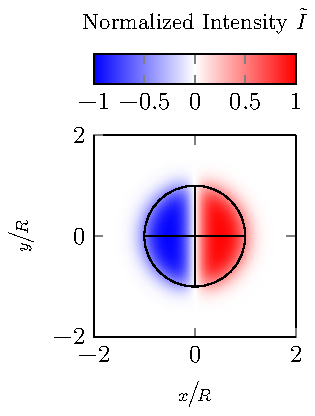
\includegraphics[]{Plots/cache/QPDx.pdf}
    \caption{Caption}
    \label{fig:T_xQPD}
  \end{subfigure}
  \hfill
  \begin{subfigure}[b]{0.3\textwidth}
    \centering
    % \tikzsetnextfilename{QPDy}

\renewcommand{\tikzHelper}{
  \draw[black] (-1,0,0)--(1,0,0);
  \draw[black] (0,-1,0)--(0,1,0);
  \draw[black] (0,0,0) circle (1);

  \draw[black, dotted] (-1.5,0,0) -- (1.5,0,0);
  \draw[black, dotted] (-1.5,-0.6,0) -- (1.5,-0.6,0);
  \draw[black, dotted] (-1.5,0.6,0) -- (1.5,0.6,0);
}

\pgfplotsset{%
    colormap={bwr}{
      color=(blue);
      color=(white);
      color=(red);
    }%
}

\begin{tikzpicture}
  \begin{axis}[view={0}{90},
      xlabel=$\sfrac{x_{0}}{\RA}$,
      yticklabels={,,},
      point meta min=-1,
      point meta max=1,
      height=48mm,
      width=48mm,
      colorbar,
      colorbar horizontal,
      colorbar style={
        title={\footnotesize Normalized Intensity $\normalized{\intensity}$},
        at={(0,1.4)},
        anchor=north west,
        xtick={-1,0,1},
      }
    ]
      \addplot3[surf,mesh/rows=99,shader=interp] table[x=x,y=y,z=Vx] 
      {\relPath/10_Figures/TikZ/V_mat.dat};
    \tikzHelper
  \end{axis}
\end{tikzpicture}

    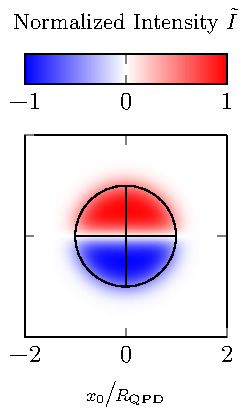
\includegraphics[]{Plots/cache/QPDy.pdf}
    \caption{Caption}
    \label{fig:T_yQPD}
  \end{subfigure}
  \hfill
  \begin{subfigure}[b]{0.3\textwidth}
    \centering
    % \tikzsetnextfilename{QPDt}

\begin{tikzpicture}
  \begin{axis}[view={0}{90},
      xlabel=$\sfrac{x_{0}}{\RA}$,
      yticklabels={,,},
      height=48mm,
      width=48mm,
      colormap name=WhiteOr,
      colorbar,
      colorbar horizontal,
      colorbar style={
        title={\footnotesize Normalized Voltage $\normalized{V}_{t}$},
        at={(0,1.4)},
        anchor=north west,
        xtick={0,0.5,1},
      }
    ]
      \addplot3[surf,mesh/rows=99,shader=interp] table[x=x,y=y,z=V] 
      {\relPath/10_Figures/TikZ/V_mat.dat};

  \draw[black] (-1,0,0)--(1,0,0);
  \draw[black] (0,-1,0)--(0,1,0);
  \draw[black] (0,0,0) circle (1);

  \draw[black, dotted] (-1.5,0,0) -- (1.5,0,0);
  \draw[black, dotted] (-1.5,-0.6,0) -- (1.5,-0.6,0);
  \draw[black, dotted] (-1.5,0.6,0) -- (1.5,0.6,0);
  \end{axis}
\end{tikzpicture}

    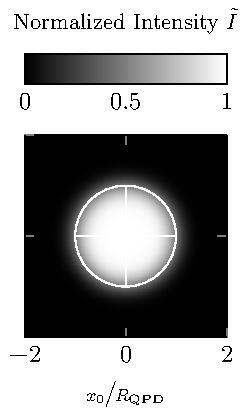
\includegraphics[]{Plots/cache/QPDt.pdf}
    \caption{Caption}
    \label{fig:T_totalQPD}
  \end{subfigure}
  \caption{QPDs}
  \label{fig:QPDs}
\end{figure}

\lipsum[1-5]

\begin{figure}[htp]
  \centering
  % \tikzsetnextfilename{Snell}

\tikzstyle arrowstyle=[scale=1]

\tikzstyle directed=[postaction={decorate,decoration={markings,
    mark=at position .65 with {\arrow[arrowstyle]{stealth}}}}]

\tikzstyle reverse directed=[postaction={decorate,decoration={markings,
    mark=at position .65 with {\arrowreversed[arrowstyle]{stealth};}}}]

\tikzset{SnellNode/.style={text width=10mm, align=center}}

\begin{tikzpicture}
  \def\W{5}
  \def\H{4}
  \def\x{0.95}
  \def\anglealpha{0}
  \pgfmathsetmacro{\y}{{(1-\x)*\H}}
  \pgfmathsetmacro{\radius}{(\W^2+\y^2)/2/\y}
  \pgfmathsetmacro{\anglealpha}{{asin(\W/\radius)}}
  \pgfmathsetmacro{\s}{{90+\anglealpha}}
  \pgfmathsetmacro{\e}{{90-\anglealpha}}

  \pgfmathsetmacro{\anglebeta}{{0.8*\anglealpha}}
  \pgfmathsetmacro{\p}{{(\radius-\H)*sin(\anglebeta)}}
  \pgfmathsetmacro{\px}{{\radius*sin(\anglebeta)}}
  \pgfmathsetmacro{\py}{{-\radius*(1-cos(\anglebeta))}}


  % define coordinates
  \coordinate (O) at (0,0) ;
  \coordinate (A) at (0,\H) ;
  \coordinate (B) at (0,-\H) ;

  % media
  \fill[blue!20,opacity=.3] (-\W,0) rectangle (\W,\H);
  \fill[black!10!,opacity=.3] (-\W,0) rectangle (\W,-\H);
  \node[right, SnellNode] at (3,1.5) {{Fluid\\ $\nf$}};
  \node[left, SnellNode] at (-2,-2) {{Particle\\ $\ns$}};

  % axis
  \draw[dash pattern=on5pt off3pt] (A) -- (B) ;
  % normal
  \draw[|->, thick] (0,0) -- node[right, pos=1] {$\normalvector$} (0, 2.5);


  % ray representation
  \def\gamma{130}
  \draw[red, variable=\x, domain=2.5:\W, samples=100] (0,\H) plot 
  ({\x*cos(\gamma)-cos(\x*pi r*3)/4*sin(\gamma)},{sin(\gamma)*\x+cos(\x*pi 
  r*3)/4*cos(\gamma)});

  % rays
  \draw[red,ultra thick,reverse directed] (O) -- node[left, xshift=-1mm, 
  pos=0.2] {$P_{\MR{i}}$} (130:5.2);

  \draw[red,ultra thick,directed] (O) -- node[right, xshift=1mm, pos=0.2] 
  {$P_{\MR{r}}$} (50:5.2);

  \draw[red,thick,dotted] ([xshift=1cm]O) -- ([xshift=1cm]130:5.2);
  \draw[red,thick,dotted] ([xshift=1cm]O) -- ([xshift=1cm]50:5.2);

  \draw[red,|<->|,>=stealth'] (130:3) -- node[above,pos=0.2,yshift=1mm] 
  {$w_{\MR{i}}$} ++(+40:0.775);
  \draw[red,|<->|,>=stealth'] (50:4) -- node[above,pos=0.7] {$w_{\MR{r}}$} 
  ++(-40:0.775);

  \draw[blue,directed,ultra thick] (O) -- node[right, xshift=1mm, pos=0.2] 
  {$P_{\MR{t}}$} (-70:4.24);

  \draw[blue,thick,dotted] ([xshift=1cm]O) -- ([xshift=1cm]-70:4.24);

  \draw[blue,|<->|,>=stealth'] (-70:3) -- node[above,pos=0.4] {$w_{\MR{t}}$} 
  ++(20:0.945);

\draw[thick,|<->|,>=stealth'] (O) -- node[midway,below] {$w$} ++(1,0);

  % particle circumference
  \draw (-\W,-\y) arc (\s:\e:\radius);
  \draw[black,->|,>=stealth'] (\p,-\H) -- node[right, pos=0.7] {$\R$} (\px, 
  \py);

  % angles
  \draw[->,>=stealth'] (0,1) arc (90:130:1);
  \draw[->,>=stealth'] (0,1) arc (90:50:1);
  \draw[->,>=stealth'] (0,-1.4) arc (270:290:1.4);

  \node[] at (280:1.8)  {$\transmitted$};
  \node[] at (110:1.4)  {$\incident$};
  \node[] at (70:1.4)  {$\reflected$};

\end{tikzpicture}

  \includegraphics[]{Plots/cache/Snell.pdf}
  \caption{Caption}
  \label{fig:T_snell}
\end{figure}

\lipsum[1-5]

\begin{figure}
  \centering
  \begin{subfigure}[b]{0.45\textwidth}
    \centering
    % \tikzsetnextfilename{gamma}
%%%%%%%
% READ TABLE
%%%%%%%

\begin{tikzpicture}
    \begin{axis}[view={0}{90},
        xlabel={$a$ [-]},
        ylabel={$\beta$ [\si{\degree}]},
        xmax=0.5,
        height=60mm,
        point meta min=0,
        point meta max=72,
        width=60mm,
        colormap name=viridis,
        colorbar,
        colorbar horizontal,
        colorbar style={
          title={$\gamma$ [\si{\degree}]},
          at={(0,1.3)},
          anchor=north west,
          xtick={0,24,48,72},
        },
        ytick={0,24,48,72},
        xtick={0,0.25,0.5},
      ]
      \addplot3[surf,mesh/rows=51,shader=interp] table[x=a,y=beta,z=gamma] 
      {\relPath/10_Figures/TikZ/angles_mat.dat};
    \end{axis}
\end{tikzpicture}

    \includegraphics[]{Plots/cache/gamma.pdf}
    \caption{Caption}
    \label{fig:T_gamma}
  \end{subfigure}
  \hfill
  \begin{subfigure}[b]{0.45\textwidth}
    \centering
    % \tikzsetnextfilename{theta_i}
%%%%%%%
% READ TABLE
%%%%%%%

\begin{tikzpicture}
    \begin{axis}[view={0}{90},
        xlabel={$a$ [-]},
        ylabel={$\beta$ [\si{\degree}]},
        xmax=0.5,
        height=60mm,
        point meta min=0,
        point meta max=30,
        width=60mm,
        colormap/YlGnBu-9,
        colorbar,
        colorbar horizontal,
        colorbar style={
          title={$\incident$ [\si{\degree}]},
          at={(0,1.3)},
          anchor=north west,
          xtick={0,10,20,30},
        },
        ytick={0,24,48,72},
        xtick={0,0.25,0.5},
      ]
      \addplot3[surf,mesh/rows=51,shader=interp] table[x=a,y=beta,z=theta] 
      {\relPath/10_Figures/TikZ/angles_mat.dat};

      % lines
       \addplot3[
         mesh/rows=51,
         mesh/cols=50,
         contour gnuplot={levels={1,2,5,15,10,20},draw color=black},
     ] table[x=a,y=beta,z=theta] {\relPath/10_Figures/TikZ/angles_mat.dat};
    \end{axis}
\end{tikzpicture}

    \includegraphics[]{Plots/cache/theta_i.pdf}
    \caption{Caption}
    \label{fig:T_theta_i}
  \end{subfigure}
  \caption{angles}
  \label{fig:T_gamma_theta}
\end{figure}

\lipsum[1-5]

\begin{figure}[htp]
  \centering
  % \tikzsetnextfilename{voltages_over_x}
%%%%%%%
% READ TABLE
%%%%%%%
\pgfplotstableread{\relPath/10_Figures/TikZ/V_line.dat}{\data}

\renewcommand{\tikzHelper}{
    \filldraw[black!10!, opacity=0.5] (-1,-1.1) rectangle (1,1.1);
    \filldraw[black!30!, opacity=0.5] (-0.15,-1.1) rectangle (0.15,1.1);
}

\begin{tikzpicture}
\begin{groupplot}[
    group style={
        group name=myplot,
        group size= 1 by 3,
        vertical sep=8mm,
        },
    height=40mm,
    width=120mm,
    ymin=-1.1,
    ymax=1.1,
    % legend style={fill=black,draw=white,},
    ]
    \nextgroupplot[
    % ylabel={$\tilde{I}$},
      xticklabels={,,},
      title={$y_{0} = \sfrac{0.6}{\RA}$},
      title style={yshift=-2mm},
      ]
      \tikzHelper
      \addplot[] table[x=x,y=Vy_3] {\data};
      \addlegendentry{$V_{\MR{x}}$};
      \addplot[dotted] table[x=x,y=Vx_3] {\data};
      \addlegendentry{$V_{\MR{y}}$};
      \addplot[dashed] table[x=x,y=V_3] {\data};
      \addlegendentry{$V_{\MR{t}}$};

      \draw[ultra thick, red, dashdotted] (axis cs:-0.4,-1.4026) -- (axis 
      cs:0.4,1.4026);

    \nextgroupplot[
      % ylabel={$\tilde{I}$},
      title={$y_{0} = \sfrac{0}{\RA}$},
      title style={yshift=-2mm},
      xticklabels={,,},
      ylabel={Normalized Intensity $\normalized{\intensity}$},
      every axis y label/.append style={at=(ticklabel cs:0.5)}
      ]
      \tikzHelper
      \addplot[] table[x=x,y=Vy_2] {\data};
      \addplot[dotted] table[x=x,y=Vx_2] {\data};
      \addplot[dashed] table[x=x,y=V_2] {\data};

      \draw[ultra thick, red, dashdotted] (axis cs:-0.4,-1.4795) -- (axis 
      cs:0.4,1.4795);
    \nextgroupplot[
      % ylabel={$\tilde{I}$},
      xlabel={$\sfrac{x_{0}}{\RA}$},
      title={$y_{0} = \sfrac{-0.6}{\RA}$},
      title style={yshift=-2mm},
      ]
      \tikzHelper
      \addplot[] table[x=x,y=Vy_1] {\data};
      \addplot[dotted] table[x=x,y=Vx_1] {\data};
      \addplot[dashed] table[x=x,y=V_1] {\data};

      \draw[ultra thick, red, dashdotted] (axis cs:-0.4,-1.4026) -- (axis 
      cs:0.4,1.4026);
\end{groupplot}
\end{tikzpicture}

  \includegraphics[]{Plots/cache/voltages_over_x.pdf}
  \caption{Fresnel}
  \label{fig:T_voltages_over_x}
\end{figure}

\lipsum[1-5]

\begin{figure}[htp]
  \centering
  % \tikzsetnextfilename{Fresnel}
%%%%%%%
% READ TABLE
%%%%%%%
\pgfplotstableread{\relPath/10_Figures/TikZ/Fresnel.dat}{\data}

\begin{tikzpicture}
  \begin{groupplot}[
    axis on top=true,
    group style={
      group size=2 by 1,
      horizontal sep = 13mm,
    },
    xmin=0,
    ymin=0,
    height=55mm,
    width=83mm,
    no markers,
  ]
  \nextgroupplot[
    xlabel={Incident angle $\incident$ [\si{\degree}]},
    ylabel={\footnotesize Fresnel Coefficient [-]},
    xtick={0,0.16666,0.333333,0.5},
    xticklabels={0, 30, 60, 90},
    legend style={
      at={(axis cs:0.01,0.5)},
      anchor=west,
      font=\footnotesize,
    }
  ]
  \filldraw[black!10!,opacity=0.7] (0.155,0) rectangle ({0.5,1}|-{rel axis 
  cs:1,1});

    \addplot[dashed] table[x=theta,y=R_M2P] {\data};
    \addlegendentry{$\fresnelR_{\mathrm{f\rightarrow s}}$};
    \addplot[] table[x=theta,y=T_M2P] {\data};
    \addlegendentry{$\fresnelT_{\mathrm{f\rightarrow s}}$};

    \addplot[thick, blue, dotted] table[x=theta,y=R_P2M] {\data};
    \addlegendentry{$\fresnelR_{\mathrm{s\rightarrow f}}$};
    \addplot[thick, blue] table[x=theta,y=T_P2M] {\data};
    \addlegendentry{$\fresnelT_{\mathrm{s\rightarrow f}}$};

    \nextgroupplot[
    xlabel={Incident angle $\incident$ [\si{\degree}]},
    xmax=0.167,
    ymin=0.001,
    ymode=log,
    xtick={0,0.05555,0.11111,0.1666666},
    xticklabels={0, 10, 20, 30},
  ]

  \filldraw[black!10!,opacity=0.7] (0.155,0.00001) rectangle ({0.167,1}|-{rel 
  axis cs:1,1});

    \addplot[dashed] table[x=theta,y=R_M2P] {\data};
    \addplot[] table[x=theta,y=T_M2P] {\data};

    \addplot[thick, blue, dotted] table[x=theta,y=R_P2M] {\data};
    \addplot[thick, blue] table[x=theta,y=T_P2M] {\data};

  \end{groupplot}
  % \draw[thick,blue,->,shorten >=2pt,shorten <=2pt] (group c1r1.east) -- (group 
  % c2r1.west);
\end{tikzpicture}

  \includegraphics[]{Plots/cache/Fresnel.pdf}
  \caption{Fresnel}
  \label{fig:T_fresnel}
\end{figure}

\lipsum[1-5]

\begin{figure}[htp]
  \centering
  % \tikzsetnextfilename{angles}

\tikzstyle arrowstyle=[scale=2]
\tikzstyle directed=[postaction={decorate,decoration={markings,
    mark=at position .65 with {\arrow[arrowstyle]{stealth}}}}]

\pgfmathsetmacro{\R}{5}     % COS
\pgfmathsetmacro{\ytop}{4}     % COS
\pgfmathsetmacro{\ybot}{-0.5}     % COS

\begin{tikzpicture}[scale=1.3]
    \coordinate (O) at (0,0);
    \coordinate (I) at (4,3);
    \coordinate (A) at (0,1.4);

    \begin{scope}
      \clip (-1,\ybot) rectangle (6,\ytop);
      \fill[colFluid,opacity=0.3] (-1,\ybot) rectangle (6,\ytop);
      \fill[white] (O) circle (\R);
      \fill[colParticle,opacity=0.3] (O) circle (\R);
    \end{scope}

    \node[circle,fill=black,inner sep=0pt,minimum size=3pt,label=below:{$M$}] 
    at (O) {};
    \node[circle,fill=black,inner sep=0pt,minimum size=3pt,label=left:{$f$}] at 
    (A) {};
    \node[circle,fill=black,inner sep=0pt,minimum size=3pt,label=above:{$A$}] 
    at (I) {};

    % \draw (O) -- node[midway, below, xshift=1mm] {$R$} (I) -- node[above, 
    % midway, xshift=-1mm] {$y$} (A) -- node[midway, left] {$a\,R$} cycle;
    \draw (O) -- node[midway, below, xshift=1mm] {$R$} (I) -- (A) -- 
    node[midway, left] {$\Rprime$} cycle;

    % \draw[dotted] (O) rectangle (I);
    \draw[dotted] (A) -- ++(0,1);

    \draw[->,>=stealth'] (I) -- node[above,midway] {$\normalvector$} (36.86:6);

    \draw[directed,red] (34.0:6.2) -- (I);


    \draw[] (0,0.5) arc (90:37:0.5) node[midway, above] {$\gamma$};
    \draw[] (0,1.9) arc (90:22:0.5) node[midway, above] {$\beta$};
    \draw[] (0,1.1) arc (-90:22:0.3) node[midway, right] 
    {$\sfrac{\pi}{2}-\beta$};
    \draw[] (36.8:3.5) arc (216:200.5:1.5) node[pos=.3, left] {$\incident$};

    % particle surface
    \pgfmathsetmacro{\res}{asin(\ytop/\R}
    \draw[] (I) arc (36.86:\res:\R);
    \pgfmathsetmacro{\res}{asin(\ybot/\R}
    \draw[] (I) arc (36.86:\res:\R);

    % nodes
    \node[align=center,text width=15mm] at (5.3,2) {{fluid\\ $\nf$}};
    \node[align=center,text width=15mm] at (3,0) {{particle\\ $\ns$}};


\end{tikzpicture}

  \includegraphics[]{Plots/cache/angles.pdf}
  \caption{Caption}
  \label{fig:T_angles}
\end{figure}

\lipsum[1-5]

\begin{figure}[htp]
  \centering
  % \tikzsetnextfilename{ray}

\tikzset{cross/.style={
  cross out,
  draw=black,
  minimum size=2*(#1-\pgflinewidth),
  inner sep=0pt, outer sep=0pt},
  cross/.default={1pt}}

\tikzstyle arrowstyle=[scale=2]

\tikzstyle directed=[postaction={decorate,decoration={markings,
    mark=at position .5 with {\arrow[arrowstyle]{stealth}}}}]

\tikzstyle reverse directed=[postaction={decorate,decoration={markings,
    mark=at position .65 with {\arrowreversed[arrowstyle]{stealth};}}}]

\begin{tikzpicture}[scale=1.5]

  % define coordinates
  \coordinate (O) at (0,0) ;
  \coordinate (F) at (0,0.15) ;
  \coordinate (N) at (260:2) ;

  % medium
  \filldraw[blue!20!, opacity=0.3] (-3,-3) rectangle ++(6,6);


  % particle
  \draw[fill=white] (O) circle (2);
  \draw[fill=black!10!, opacity=0.3] (O) circle (2);

  \node[circle, fill=black, inner sep=0pt, minimum size=3pt, label=left:{$M$}] 
  at (O) {};
  \node[circle, fill=black, inner sep=0pt, minimum size=3pt, label=above:{$f$}] 
  at (F) {};

  % rays
  \coordinate (I) at (28.6:2) ;
  \draw[directed,red] (2.5,1.3) -- node[below, midway] {$P^{1}_{\mathrm{i}}$} 
  (I);
  \draw[directed,red] (N) -- node[left,xshift=-0.1mm] {$P^{2}_{\mathrm{t}}$} 
  (258:2.8);

  \draw[directed, blue] (I) -- node[right,midway,xshift=0.1mm] 
  {$P^{1}_{\mathrm{t}}=P^{2}_{\mathrm{i}}$} (N);

  \draw[directed, blue] (N) -- node[left,midway,xshift=-0.1mm] 
  {$P^{2}_{\mathrm{r}}=P^{3}_{\mathrm{i}}$} (131.4:2);

  % arcs
  \draw[<-,>=stealth'] ([shift=(234:0.5)]I) arc (234:209:0.5);

  \draw[<->,>=stealth'] ([shift=(55:0.5)]N) arc (55:105:0.5);

  \node[] at (22:1.2) {$\transmitted^{1}$};
  \node[] at (269:1.2) {$\incident^{2}$};
  \node[] at (254:1.22) {$\refracted^{2}$};

  % middle to hitting point
  \draw[densely dotted] (O) -- node[below,pos=0.3] {$\R$} (I);
  \draw[densely dotted] (O) -- node[left,pos=0.3] {$\R$} (N);
  \draw[red, dotted] (I) -- (F);
  % surface normal
  \draw[|->,>=stealth'] (N) -- node[right,pos=0.9] {$\normalvector$} (260:3);
  \draw[|->,>=stealth'] (I) --node[above,pos=0.9] {$\normalvector$} (28.6:3);

  % text
  \node[align=center, text width=10mm] at (-0.5,1) {{Particle\\ $\ns$}};

  \node[align=center, text width=10mm] at (1.5,2) {{Fluid\\ $\nf$}};




\end{tikzpicture}

  \includegraphics[]{Plots/cache/ray.pdf}
  \caption{Caption}
  \label{fig:T_ray_particle}
\end{figure}


\cleardoublepage
\renewcommand{\relPath}{SECTION/30_Timeconstant}
 
\chapter[Dynamic Timeconstant Measurement]{Dynamic Measurement of the Acoustic 
Streaming Time Constant utilizing an Optical Tweezer}\label{ch:timeconstant}
\textit{This chapter is original work by Christoph Goering:
\footnote{: DOI: 10.1103/PhysRevE.104.025104, reproduced under the terms of the 
Creative Commons Attribution 4.0 license.}}

\vspace{5mm} \noindent
C. Goering and J. Dual, "Dynamic measurement of the acoustic streaming time 
constant utilizing an optical tweezer", Physical Review E, 2021, \textbf{104}, 
025104.


\section{Abstract}
The combination of a bulk acoustic wave device and an optical trap allows 
studying the build up time of the respective acoustic forces. In particular, we 
are interested in the time it takes to build up the acoustic radiation force 
and acoustic streaming. For that, we measure the trajectory of a spherical 
particle in an acoustic field over time. The shape of the trajectory is 
determined by the acoustic radiation force and by acoustic streaming; both 
acting on different time scales. For that, we utilize the high temporal 
resolution ($\Dt = \SI{0.8}{\us}$) of an optical trapping setup. With our 
experimental parameters the acoustic radiation force on the particle and the 
acoustic streaming field theoretically have characteristic build up times of 
\SI{1.4}{\us} and \SI{1.44}{\ms}, respectively. By choosing a resonance mode 
and a measurement position where the acoustic radiation force and acoustic 
streaming induced viscous drag force act in orthogonal directions, we can 
measure the evolution of these effects separately. Our results show, that the 
particle is accelerated nearly instantaneously by the acoustic radiation force 
to a constant velocity, whereas the acceleration phase to a constant velocity 
by the acoustic streaming field takes significantly longer. We find that the 
acceleration to a constant velocity induced by streaming takes in average about 
17'500 excitation periods ($\approx \SI{4.4}{\ms}$) longer to develop than the 
one induced by the acoustic radiation force. This duration is about 4 times 
larger than the so-called momentum diffusion time which is used to estimate the 
streaming build up. In addition, this rather large difference in time can 
explain why a pulsed acoustic excitation can indeed prevent acoustic streaming 
as it has been shown in some previous experiments.

\section{Introduction\label{sec:introduction}}

In recent years, acoustofluidics has provided many powerful tools. Due to being 
contact-less, label-free, and biocompatible 
\cite{Antfolk2015,Abdulla2020,Zielke2020,Binkley2020,Cai2020}, acoustofluidic 
manipulation can be used in medical applications for cancer research
\cite{Antfolk2015,Abdulla2020,Zielke2020,Binkley2020}, Alzheimer research 
\cite{Cai2020}, targeted drug delivery \cite{Bose2015}, and for pumping medical 
fluids \cite{Wu2019}. In addition, there are biological 
\cite{Gerlt2020,Xie2019} and engineering applications (e.g., micro-pumping 
\cite{Wu2019,Huang2014,Lin2019,Ozcelik2021}).

Most of these applications utilize the acoustic radiation force (ARF) to 
manipulate objects on the micro-scale. The ARF is a second-order time-averaged 
effect that arises from the interaction of an acoustic field scattered at an 
object surface and a background acoustic field 
\cite{Doinikov1994,Hasegawa1969,Yosioka1955,Gorkov1962,Bruus2012}.
These objects can be solid particles, air bubbles, fluid droplets, biological 
samples, as long as their material properties (density $\rho$ and speed of 
sound $c$) are different from the surrounding medium. However, there coexists 
a fluid motion called acoustic streaming (AS) 
\cite{Nyborg1965,Kolb1956,Nyborg1953}. This motion can arise either from
viscous losses in the fluid (Eckhart type streaming \cite{Eckart1948}) or it 
can arise in the viscous boundary layer at a fluid to wall interface 
(Schlichting and Rayleigh streaming \cite{Riley1998,Schlichting1932}).


The theoretical derivations usually describe the steady-state of the AS field. 
A theoretical numerical study \cite{Muller2015} investigated the temporal build 
up of the ARF and AS field. In contrast to the ARF, the viscous drag force 
arising from AS is independent of the object material properties because it is 
a motion of the fluid. The AS direction coincides with the direction of the 
relative motion between fluid and particle.

For a spherical object of radius $R$, the drag force in laminar flow scales 
linearly with the object radius $\FAS \propto R$. In contrast to the $\FAS$, 
the ARF scales with the volume $\FARF \propto \R^{3}$ \cite{Bruus2012-10}.  
Based on the fluid and the object material properties, the $\FARF$ will 
dominate over the $\FAS$ if the radius $\R$ is greater than the critical radius 
$\R_{\text{crit}}$, where $\FAS = \FARF$ holds. The direction of $\FAS$ can be 
different from the $\FARF$. Therefore, the $\FAS$ is usually undesired.

The ARF and the AS occur not only in the bulk of the fluid, but also on sharp 
edges of a device \cite{Doinikov2020a,Doinikov2020b,Leibacher2015,Nama2016}. 
So-called micro-streaming around the surface of a spherical particle can even 
cause a sign inversion of the ARF if the viscous boundary layer $\delta$ is 
sufficiently large \cite{Baasch2019}. However, there are applications that take 
advantage of the AS \cite{Antfolk2014,Mao2017,Hao2020}: a complete overview of 
AS applications can be found in \cite{Wiklund2012a}.

In literature, it is well understood how long it takes until the acoustic 
field, and hence the ARF, needs to build up \cite{Muller2015} and how long the 
particle focusing takes \cite{Bruus2012-10}. However, it is still not fully 
clear how long it takes for the AS to build up, and what the definition for the 
analytical AS time constant is. In the acoustofluidics community, it is 
generally accepted that the build up for the AS field takes longer than the 
build up of the ARF. By using a pulsed actuation of the acoustic field and 
therefore exploiting this time offset, \citeauthor{Hoyos2013} prevented the 
build up of AS \cite{Hoyos2013,Castro2016}. They varied the number of periods 
for which the acoustic actuation is switched on and off, respectively. They 
experimentally showed that for a ratio of about 1 to 1 between 500 on- and 500 
off-periods the streaming velocity is less than 50\% of its steady-state 
magnitude while the ARF is not affected by that much.

\citeauthor{Muller2015} studied the build up of the acoustic energy density and 
streaming velocity with a numerical model \cite{Muller2015}. Their model 
consisted of a fluid cavity without any surrounding structure such as the 
cavity walls. They found numerically that indeed the ARF builds up 
significantly faster than the AS. However, the simulations with a pulsed 
actuation of different ratios of on- to off-periods did not prevent the build 
up of AS because its decay -- as the build up -- is slow compared to the ARF. 
The streaming builds up significantly slower during the on-periods, however, it 
does not decay to its initial value during the off-periods. Over time the 
influence of AS increases because the ARF alternates between some magnitude in 
the on-periods and zero in the off-periods. This implies, that the simulation 
of \citeauthor{Muller2015} could not explain the experimental results by 
\citeauthor{Hoyos2013}.

In this work, we experimentally measure the time until a \Dtwo~spherical 
silicon-dioxide (\SiO) particle moves with constant velocity when accelerated 
by the ARF and AS. Instead of using a camera, we utilize a data acquisition 
board (DAQ) with a sampling frequency of $f_{\text{s}} = \SI{1.25}{\MHz}$ to 
measure the relative particle trajectory as soon as the ultra-sound (US) is 
switched on. This high sampling frequency $f_{\text{s}}$ yields a high 
temporal resolution of $ \Dt = \SI{0.8}{\us}$. Considering the acoustic 
excitation frequency $\fex = \SI{4.015}{\MHz}$, we sample at least every fourth 
excitation period.

The optical tweezer (OT) for this study has already been successfully applied 
in the fields of acoustofluidics for stationary force measurements within a 
microfluidic chip \cite{Lamprecht2016,Lakaemper2015} as well as acoustic 
viscous torque investigations \cite{Lamprecht2021}. Here, we characterize in a 
first step the stationary force field in the bulk of the device to ensure, that 
we measure in a second step the time resolved build up of AS and the ARF 
separately and not their superposition. The separation is done by choosing a 
particle position within the acoustic field, where the $\FAS$ and $\FARF$ are 
orthogonal to each other. In order to measure in the second step solely the 
effects of the acoustic field on the particle and not the characteristics of 
the OT, we alter the usual trapping setup. The modification is that the 
particle is released from the OT before the acoustic excitation starts and 
retrapped after it.  Hence, during the measurement just gravity and the forces 
of the acoustic field act upon the particle. With our modified trapping setup, 
we are able to measure precisely the ARF and AS induced movement of a single 
particle in the bulk of the fluid.

Our manuscript is structured as follows: in \cref{sec:theory} we derive and 
list all time constants in our system and we compute the traveled distances of 
a free floating particle in an acoustic field. Those influences need to be 
considered for our measurement protocol. In addition, we perform numerical AS 
simulations of our device to further understand the AS field; in 
\cref{sec:experimental-setup} we explain our experimental setup and its 
modifications; in \cref{sec:experimental-procedure} we show the results of the 
stationary force measurement, before explaining our time evolution measurement 
protocol and the data post-processing; and in \cref{sec:results} we show and 
discuss the results of this study.




\section{Theory \label{sec:VT-theory}}

Two orthogonal standing waves excited at the same frequency $f$ and with a 
relative phase shift $\zeta$ exert a torque on spherical particles. Under these 
conditions, an acoustic streaming field is formed inside the viscous boundary 
layer

\begin{equation}
    \delta = \sqrt{\frac{\mu_{f}}{\rho_{f}\,\pi\,f}}
    \label{eq:VT-delta}
\end{equation}

at the fluid-particle interface, where $f$ is the frequency (of excitation), 
$\mu_{f}$ the dynamic fluid viscosity, and $\rho_{f}$ the density of the fluid. 
The resulting viscous surface stress on the particle results in a non-zero 
torque. This torque is called the acoustic VT and is qualitatively shown in 
\cref{fig:VT-Fig1} for two orthogonal standing waves with a phase shift of 
$\zeta = \sfrac{\pi}{2}$.

%%%%%%%%%%%
\begin{figure}
    \centering
    \includegraphics[width=100mm]{\relPath/10_Figures/Fig1.png}
    \caption{Schematic of the time-averaged acoustic VT acting on a sphere. At a 
    constant rotational rate $\Omega$ of the particle the propulsive acoustic 
  VT is in balance with its counteracting viscous drag 
  torque.\label{fig:VT-Fig1}}
\end{figure}%
%%%%%%%%%%%

The analytical solution for the total time-averaged VT 
$\Gamma_{\text{tot}}(\Omega)$ on a small rotating spherical particle 
($R\ll\lambda=\sfrac{c_f}{f}$) within two orthogonal plane standing waves is 

%%%%%%%%%%%%%%%%%%%
\begin{equation}
  \label{eq:VT-Eq1}
  \begin{split}
      &\Gamma_{\text{tot}}(\Omega) = \\
      &= \frac{3}{4} \frac{\delta S_s A_{X} A_{Y}}{\rho_{f} c_{f}^{2}} \sin\zeta \cos(kX) \cos(kY) - 8 \pi \mu_f R^3\,\Omega \\
     &= \Gamma_{\text{IN}} - \tilde{D}\,\Omega
   \end{split}
 \end{equation}
%%%%%%%%%%%%%%%%%%%
where $S_s$ is the sphere surface area, and $c_f$ the speed of sound of the 
fluid, $k=\sfrac{2\pi}{\lambda}$ the wavenumber in the fluid, and ($A_{X}$; 
$A_{Y}$) the pressure amplitudes of the two orthogonal standing waves 
\cite{Wang1989, Lamprecht2013}.  The phase shift $\zeta$ and the sphere position 
($X$;$Y$) determine the rotation direction.  The result of 
$\Gamma_{\text{tot}}(\Omega)$ can be split up into a torque driven by the 
acoustic excitation $\Gamma_{\text{IN}} \propto R^{2}$ and a viscous drag torque 
$\tilde{D}\,\Omega \propto R^{3}$ related to Stokes drag \cite{Lamprecht2013}. In 
the theory of \citeauthor{Nyborg1958} \cite{Nyborg1958} and \citeauthor{Wang1989} 
\cite{Wang1989}, the particle rotation was not considered in their analysis of the 
acoustic VT $\Gamma_{\text{IN}}$.  However, \citeauthor{Lamprecht2013} 
\cite{Lamprecht2013} introduced a moving boundary of the particle so that the 
driving $\Gamma_{\text{IN}}$ appears independently of the rotational rate 
$\Omega$. The rotational axis of the particle is always perpendicular to both 
directions of the incident waves and its rotational rate is limited by Stokes 
drag coefficient $\tilde{D} = 8 \pi \mu_f R^3$. The steady-state rotational rate 
$\finalOmega$ is defined as
%%%%%%%%%%%%%%%%%%%
\begin{equation}
  \label{eq:VT-AcGovEqConti}
  \finalOmega=\frac{\Gamma_{\text{IN}}}{\tilde{D}}.
\end{equation}
%%%%%%%%%%%%%%%%%%%
Since $\finalOmega \propto \sfrac{1}{R}$ \cite{Lamprecht2013}, bigger particles will 
reach a lower steady-state rotational rate $\finalOmega$. This occurs for the 
equilibrium state $\Gamma_{\text{IN}}(t=t^\star)= \tilde{D} (t = t^\star )$.  
After $ t^\star = \SI{0.5}{\milli\second}$ a \SI{100}{\micro\meter} large 
particle rotates with the steady-state rate of $\SI{11.33}{\hertz}$
(\SI{680}{\rpm}) at an acoustic pressure amplitude of \SI{171}{\kilo\pascal} 
\cite{Lamprecht2015}. Please note that the time constant $\tau \approx 
t^{\star}$ is proportional to $R^2$ \cite{Lamprecht2015}, so a particle with 
$2\,R=\SI{2.06}{\um}$ reaches the equilibrium in less than 
\SI{1}{\micro\second}. \citeauthor{Hahn2016} \cite{Hahn2016} showed numerically 
that the analytical and the numerical results can differ by orders of magnitude 
for $\normBdLayer > 1$ and water as fluid. For acoustic particle manipulation in 
water, the differences between the analytical solution and the numerical results 
become negligible for particles with a normalized viscous boundary layer 
$\normBdLayer < \sfrac{1}{15}$. In addition, the analytical predictions neglect 
the density ratio $\tilde{\rho} = \sfrac{\rho_{\text{s}}}{\rho_{\text{f}}}$ 
between the particle and the surrounding fluid.  \citeauthor{Hahn2016} 
\cite{Hahn2016} concluded that the density ratio $\tilde{\rho}$ has a 
non-negligible effect on the magnitude of the acoustic VT and that depending on 
this ratio even the direction of the torque can change.

\section{Experimental Setup\label{sec:TC-experimental-setup}}

\subsection{Optical Trap Setup}

Our OT has already been applied in several other publications 
\cite{Lamprecht2021,Lamprecht2017,Lamprecht2016,Lakaemper2015} to the field of 
ARF and AS measurements in bulk acoustic wave (BAW) devices. All components are 
described there extensively. We highlight here the position detection system 
and the modifications from the force measurement setup that were necessary for 
this study. These modifications are needed because we use one \SI{785}{\nm} 
near-infrared diode laser (LuxX 785-200, Omicron Laser, Rodgau-Dudenhofen, 
Germany) for the optical trapping and also for the optical position detection.  
We detect the position of the trapped particle relative to the trap center by 
monitoring the voltages of two quadrant photo diodes (QPD) placed in the back 
focal plane (see \cref{fig:TC-laserpath}). It is possible to resolve the movement 
of the particle in all three dimensions. However, the in-plane ($xy$) and the 
axial ($z$) position detection differ.

\begin{figure}[H]
  \centering
  \def\svgwidth{85mm}
  \svginput{\relPath/10_Figures/LaTeX/Microscope.pdf_tex}
  \caption{Shutter location in laser path and schematic of laser path through 
  microscope setup; full details on the setup in 
  \cite{Lamprecht2016,Lamprecht2017}.}\label{fig:TC-laserpath}
\end{figure}

For the $xy$ position the laser beam is focused onto the QPDxy (see also 
\cref{fig:TC-laserpath}) such that the spot diameter is about five times smaller 
than the opening aperture of the QPDxy \cite{Lamprecht2017}. An in-plane 
movement of the trapped particle changes the spot location on the QPDxy which 
results in a voltage change on the four quadrants. As long as the spot is 
within the QPD opening the spatial movement is linearly related to the QPD 
voltage. By summing and subtracting these four voltages from each other, one 
can get the values corresponding to a movement along $\ex$ and $\ey$ separately 
\cite{Lamprecht2017}.

For the axial $z$ position a second QPD is needed and this QPD is overfilled 
with the laser spot (see also \cref{fig:TC-laserpath}). When the particle moves 
axially the spot diameter changes its size. If the diameter decreases more 
intensity is measured by QPDz and leads to a higher voltage and vice versa. For 
small movements ($\Dz < \R$) the relation is linear \cite{Dreyer2004}.

When converting the measured voltage changes from QPDxy and QPDz to the 
particle displacement with unit of meters, the $xy$ voltage and the $z$ voltage 
have different scaling. The three voltage-meter conversion factors are found by 
calibrating the OT via the power spectrum analysis of the trapped particle 
Brownian motion \cite{Lamprecht2021,Lamprecht2016,Lakaemper2015}.

As discussed before, the time constant $\tOT$ of the OT is larger than the 
time constant for the ARF and AS (see \cref{tab:TC-time-constants}). Therefore, we 
need to switch the laser off and then monitor the particle trajectory without 
the trapping forces, in order to measure the time evolution of the particle 
movement and not the time constant of the optical trap. This means, the particle 
is not stably trapped while measuring. However, we need the laser light for 
the position detection on the QPDs. Therefore, we reduce the laser power to a 
minimum such that the resulting trapping forces are negligibly small. As a 
result of the low power, the voltage magnitude decreases significantly on the 
QPDs, such that it is not measurable anymore. Thus, we exchange the neutral 
density (ND) filters from the force measurement setup 
\cite{Lamprecht2016,Lamprecht2021} with the fast optical shutter FOS-NIR(1100) 
(LC TEC, Borlänge, Sweden). This filter is specified to open from 0\% to 90\% 
transmittance in less than \SI{15}{\ms} and close from 100\% transmittance to 
10\% in less than \SI{5}{\ms}. The ND filters and the shutter are needed to 
reduce the intensity on the QPDs and prevent overexposure and hence damage. 
The transmittance of the shutter can be controlled with the applied driving 
voltage. Before and after the measurements the shutter is almost completely 
closed to mimic the ND filters and opened for the actual measurement with 
reduced laser power.

Lastly, we operate the laser in the so-called \emph{analogue modulation} mode 
such that the output laser power is proportional to an externally applied DC 
voltage which is sampled with more than \SI{1.5}{\MHz} by the laser controller 
unit. The low power mode for the position detection is operated with less than 
\SI{0.5}{\mW}. The low voltage DC signal for the laser averaged \SI{84.13}{\mV} 
with a standard deviation of \SI{0.13}{\mV} providing a very consistent voltage 
and hence laser power. With this power the trapping potential is too weak to 
keep the particle inside the focus of the laser beam in any of the three 
spatial directions. The usual laser power for the stationary force measurements 
is between \SI{100}{\mW} and \SI{175}{\mW}.

\begin{figure}[H]
  \centering
  % \tikzsetnextfilename{daq-sync}
\begin{tikzpicture}
  \tikzset{nodestyle/.style={pos=0.0, above, anchor=south west}}
  % \draw[white, fill=black!10!white] (2.5,0) rectangle ++(1.5,3.5);
  % \draw[|<->|] (2.5,3.5) -- ++(1.5,0) node[midway,above=2mm,align=center] 
  % {\small Shutter open\\US on\\laser power low};

  % \draw[|<->|] (1.0, 0.5) -- ++(6.0,0) node[midway, above] {particle is free to 
  % float and move};
  % axis system
  \draw[thick,->] (-0.2,0) -- ++(6.5,0) node[anchor=north west] {$t$ 
  [\si{\milli\second}]};

  % time ticks
  \draw (0, 2pt) -- ++(0, -4pt) node[anchor=north] {$-25$};
  \draw (1.0, 2pt) -- ++(0, -4pt) node[anchor=north] {$-24$};
  \draw (2.5, 2pt) -- ++(0, -4pt) node[anchor=north] {$0$};
  \draw (4.0, 2pt) -- ++(0, -4pt) node[anchor=north] {$30$};
  \draw (5.0, 2pt) -- ++(0, -4pt) node[anchor=north] {$55$};
  \draw (6.0, 2pt) -- ++(0, -4pt) node[anchor=north] {$75$};

  % laser power
  \draw[dashed] (-0.5,2.7) -- node[nodestyle] {$P_{\text{trapping}}$} ++(1.5,0) 
  -- ++(0,-1.0) -- node[nodestyle] {$P_{\text{measure}}$} ++(5.0,0) -- 
  ++(0,1.0) -- ++(1,0) node[nodestyle] {laser};

  % shutter
  \draw[dotted] (-0.5,4) -- node[nodestyle] {closed} ++(0.5,0) -- ++(1.5,-1.5) 
  -- node[nodestyle] {open} ++(2.5,0) -- ++(1.5, 1.5) -- ++(1.5,0) 
  node[nodestyle] {shutter};

  % US
  \draw[] (-0.5, 0.2) -- node[nodestyle] {off} ++(3.0,0) -- ++(0,1) -- 
  node[nodestyle] {on} ++(2.5,0) -- ++(0,-1) -- node[nodestyle] {US} ++(1.5,0);


\end{tikzpicture}

  \includegraphics[]{Plots/cache/daq-sync.eps}
  \caption{Schematic of controller timings for the shutter, the laser, and the 
      US. During the $P_{\text{measure}}$ state the particle is not trapped by 
  the OT. In the time interval $[\SI{0}{\ms}, \SI{30}{\ms}]$ (1) the shutter is 
  fully opened, (2) the US is switched on, and (3) the particle is free to 
  move. During this interval the measurement is performed.}\label{fig:TC-daq-sync}
\end{figure}

\subsection{Controller Timing and Data Acquisition}

The data acquisition (DAQ) board NI-USB 6356 (National Instruments, Austin, TX, 
USA), the laser power, the piezo excitation voltage, and the shutter 
transmittance are actuated in a defined sequence. We use an Arduino Board with 
two 12-Bit DAC units (MCP4725, Adafruit, New York, NY, USA) for controlling the 
timing and the DC voltage for the laser. The timings are depicted in 
\cref{fig:TC-daq-sync}. For $t<-\SI{24}{\ms}$ the laser is in its high power state 
and keeps the particle fixed in position against external forces. At 
$t=\SI{-25}{\ms}$ the shutter starts opening. The opening time is specified 
with less than \SI{15}{\ms} from 0\% transmittance to 90\%. At 
$t=\SI{-24}{\ms}$ the laser power changes to its low power state. Hence, the 
particle is free to move and starts its sedimentation. At $t=\SI{0}{\ms}$ the 
US is switched on. For \SI{30}{\ms} the shutter is fully opened, the particle 
is free to move, and the US is on. Then the shutter starts to close again. In 
these \SI{30}{\ms} we measure the time evolution of the particle. At 
$t=\SI{55}{\ms}$ the US is switched off and at $t=\SI{75}{\ms}$ the laser power 
is increased to its high power state. The time between two consecutive 
measurements is greater than \SI{2}{\s}, such that the fluid within the cavity 
is fully at rest again.

\subsection{Device, Particles, and Fluid}

Our device is a glass-silicon-glass device manufactured by Gesim GmbH 
(Radeberg, Germany). The material of the two glasses is B33 from Schott (Mainz, 
Germany). A sketch is shown in \cref{fig:TC-device} and its dimensions are listed 
in \cref{tab:TC-device-dimensions}. The top glass and the fluid cavity are limited 
in the $\ez$ direction because our microscope setup cannot focus deeper than 
\SI{250}{\um} \cite{Lamprecht2016,Lamprecht2017}. We define the origin of our 
coordinate system so that $z = 0$ is in the middle of the fluid cavity and $y = 
0$ is in the middle between the silicon cavity walls. We use as a reference 
point $x = 0$ such that it is approximately in the middle of the PZT length 
$l$. For all reported measurements we use the same position $x_{\text{ref}}$ as 
reference for $x=0$.

The fluid cavity is in the middle between the two silicon layers and the 
PZT is a PZ 26 element from Meggit A/S (Kvistgaard, 
Denmark). It is glued with Epo-Tek (Billerica, MA, USA) H20S two component 
epoxy onto the device. It is located at the edge of the device in $\ey$ 
direction and centered along the long side. The small height of 
the PZT is necessary to prevent physical contact with the microscope lens.

Our particles are silicon-dioxide (\SiO) particles from (microParticles GmbH, 
Berlin, Germany) with a diameter of $D_{2}=\SI{2.06}{\um}$. For the device 
characterization we also use particles from the same manufacturer with the same 
material properties, but with a diameter of $D_{4} = \SI{4.39}{\um}$. The 
particles are immersed in filtered (\SI{0.2}{\um}) and distilled water. To 
avoid particle-particle interactions during the experiment, we keep the 
particle concentration low.

We use the \Dtwo~particles because they are the smallest particles that work 
well in our OT. In addition, the critical radius where the ARF equals the drag 
force from AS can be found via \cite{Barnkob2012}
\begin{equation}
  \R_{\text{crit}} = \sqrt{\frac{3}{\Phi}}\,\delta
\end{equation}
where $\Phi$ is the acoustic contrast factor with thermoviscous correction 
\cite{Settnes2012}




\begin{subequations}
\begin{eqnarray}
  \Phi\left( \tkappa, \trho, \tdelta \right) &=& \frac{1}{3} f_{1}\left( 
  \tkappa \right) + \frac{1}{2}\,\text{Re}\left[ f_{2}\left( \trho, 
  \tdelta\right) \right],\\
  %%%%%%
  f_{1}\left( \tkappa \right) &=& 1 - \tkappa, \quad 
  \tkappa=\frac{\kappa_{\text{p}}}{\kappa_{\text{f}}},\\
  %%%%%%
  f_{2}\left( \trho, \tdelta \right) &=& \frac{2\left[ 1-\Gamma\left( \tdelta 
  \right) \right]\left( \trho-1 \right)}{2\,\trho + 1 - 3\,\Gamma\left( \tdelta 
  \right)}, \quad \trho=\frac{\rhop}{\rhof}\\
  %%%%%%
  \Gamma\left( \tdelta \right) &=& -\frac{3}{2}\left[ 1 + \iu \left( 1 + 
  \tdelta \right) \right]\tdelta, \quad \tdelta = \frac{\delta}{R}, \quad 
  \delta = \sqrt{\frac{\muef}{\rhof\,\pi f}}.
%
\end{eqnarray}
\end{subequations}
Here $\kappa_{\text{p}}$ is the particle and $\kappa_{\text{f}}$ the fluid 
compressibility, $\delta$ the viscous boundary layer thickness, and $\iu$ the 
imaginary unit. For our parameters (see \cref{tab:TC-parameters}) 
$\R_{\text{crit}} $ is equal to \SI{0.63}{\um} and \SI{0.65}{\um}, with and 
without ($\tdelta = 0$) thermoviscous correction, respectively.

With increasing particle size, two effects take place: 1) the ratio between ARF 
($\propto \R^{3}$) and AS ($\FAS\propto \R$) magnitude increases, because of 
their respective scaling, and 2) the measurement time decreases, because a 
greater ARF leads to more displacement, which in turn makes re-trapping more 
difficult.

% \begin{equation}
%   \delta = \sqrt{\frac{\muef}{\pi\,\rhof\,\fex}}
% \end{equation}

% \begin{equation}
%   \Phi = \frac{1}{3}\left[ \frac{5\,\tilde{\rho}-2}{2\,\tilde{\rho}+1} - 
%   \tilde{\kappa} \right]
% \end{equation}



\section{Experimental Procedure\label{sec:TC-experimental-procedure}}
\afterpage{

\begin{figure}[H]
  \centering
  \includegraphics[width=\figWidthDouble]{\relPath/10_Figures/4um.pdf}
  % \input{10_Figures/PGF/4um_map.pgf}
  \caption{Measured steady-state acoustic forces for a \Dfour~particle with 
    $\fex=\SI{4.015}{\MHz}$ and $V_{\text{pp}} = \SI{10.7}{\volt}$. The top row 
    depicts the forces along $\ey$ and the bottom along $\ez$. The two columns 
    correspond to two different measurement $yz$-planes at $x=\SI{-0.1}{\mm}$ 
  and $x=\SI{0.1}{\mm}$, respectively.}\label{fig:TC-4um-map}
\end{figure}

\begin{figure}[H]
  \centering
  % \input{10_Figures/PGF/2um_map.pgf}
  \includegraphics[width=\figWidthDouble]{\relPath/10_Figures/2um.pdf}
  \caption{Measured steady-state acoustic forces for a \Dtwo~particle with 
    $\fex=\SI{4.015}{\MHz}$ and $V_{\text{pp}} = \SI{10.7}{\volt}$. The top row 
    depicts the forces along $\ey$ and the bottom along $\ez$. The two columns 
  correspond to two different measurement $yz$-planes at $x=\SI{-0.1}{\mm}$ and 
$x=\SI{0.1}{\mm}$, respectively.}\label{fig:TC-2um-map}
\end{figure}
\clearpage
}

\subsection{Stationary Force Measurement}
In preparation for the time evolution measurement, where a spatial position of 
orthogonal AS forces and ARFs is beneficial, we characterized our device with 
two sets of stationary force measurements at a constant excitation frequency. 
For those measurements the optical trapping force is greater than the acoustic 
forces. One measurement was with a \Dtwo, and the other with a \Dfour~diameter 
particle. For changing the particle size we needed to empty and refill the 
device.  We kept the ambient conditions and experiment settings between the two 
measurements as constant as possible. For the measurements with the 
\Dtwo~particle the ambient temperature was \SI{24.49}{\celsius} in average with 
a standard deviation of \SI{0.10}{\celsius} and for the measurement with the 
\Dfour~particle the average temperature was \SI{24.78}{\celsius} with a 
standard deviation of \SI{0.25}{\celsius} ensuring the same experimental 
conditions for both measurements. More details regarding the protocol of those 
measurements can be found in \cite{Lamprecht2016} by 
\citeauthor{Lamprecht2016}.

We defined two $yz$ measurement planes, with $x_{1} = \SI{-0.1}{\mm}$ and 
$x_{2} = \SI{0.1}{\mm}$, respectively. In each plane we defined a grid in 
$y_{i}\in\{-0.20,0.19,\dots,0.20\}\,\si{\mm}$ and 
$z_{j}\in\{-30,-20,\dots,30\}\,\si{\um}$. At each point $(y_{i}, z_{j})$ we 
measured the forces in all three dimensions 5 times for \SI{3}{\second} each.  
Our excitation frequency was set to $\fex = \SI{4.015}{\MHz}$ and the applied 
voltage was $U_{\text{pp}} = \SI{10.7}{\volt}$. We choose $\fex$ based on a 
frequency sweep and the corresponding maximal forces in this sweep. With the 
chosen $\fex$ and the fluid speed of sound $\cfl \approx 
\SI{1500}{\meter\per\second}$, we obtain the theoretical acoustic wavelength of 
$\lap = \sfrac{\cfl}{\fex} \approx \SI{375}{\um}$. Hence, with the frequency 
$\fex$ and a channel width of $W = \SI{3}{\mm}$, 16 pressure nodal lines are 
present. For each spatial position we averaged the forces over the 
\SI{3}{\second} timespan and also over the 5 repetitions.

\Cref{fig:TC-4um-map,fig:TC-2um-map} visualize stationary force measurement 
results as contour plots for the two particle sizes. In addition, 
\Cref{fig:TC-averaged_forces_vs_dy} depicts the measured forces in $\ey$ and 
$\ez$ directions, when the data is additionally averaged over the 7 different 
heights $\Dz$. For \Cref{subfig:TC-F_y,subfig:TC-F_z}, the left vertical axis 
is the scale for the \Dfour~particle and the right vertical axis for 
\Dtwo~particles.

In \Cref{subfig:TC-F_y} the force wavelength $\laF$ is estimated to be 
\SI{180}{\um} which is in line with the theoretical wavelength $\laF = 
\sfrac{\lap}{2}$. One can also note that the shape of two force measurements is 
consistent. The ratio of the mean maximal force amplitudes $\frac{1.25}{0.17} = 
7.13$ is about the same as the ratio of the cubed diameter
\begin{equation}
  {\left( \frac{\Dfour}{\Dtwo} \right)}^{3} \approx 2.13^{3} \approx 9.68
 \label{eq:TC-ARF-AS-scaling}
\end{equation}
Based on the theoretical scaling laws we conclude that the forces in the $\ey$ 
direction are ARF dominant.


In \Cref{subfig:TC-F_z} one can see the measured forces in $\ez$ for both particle 
sizes and both measurement $yz$ planes. As for the forces in $\ey$ direction, 
in \Cref{subfig:TC-F_y}, the forces in $\ez$ direction are averaged over all 
$\Dz$. The force magnitude for both sizes is smaller than in $\ey$ direction 
for both particle sizes. The shapes, however, are similar but not as consistent 
as in \Cref{subfig:TC-F_y}. The ratio of the mean maximal force amplitudes 
$\frac{0.25}{0.08} \approx 3.1$ is about the same as the ratio of the two 
diameters, which suggests that in the $\ez$ direction the forces on the 
particle are AS dominated (see \Cref{eq:TC-ARF-AS-scaling}).

\begin{figure}[H]
  \centering
  \begin{subfigure}{\figWidth}
    \centering
    \caption{$F_{y}$ [\si{\pico\newton}]}\label{subfig:TC-F_y}
    % \tikzsetnextfilename{avgF_y_vs_dy}
\begin{tikzpicture}
  \begin{axis}[%
      scale only axis,
      width = 60mm,
      height = 5cm,
      axis y line*=left,
      legend style={
        fill=blue!10!white,
        font=\tiny,
        at={(0.03,0.05)},
        anchor=south west},
      xlabel = {$\Dy$ [\si{\mm}]}]

    \fill[fill=black!15!white] ({axis cs:-0.06,-2}|-{rel axis cs:0,0}) 
    rectangle ({axis cs:-0.03,2}|-{rel axis cs:0,1});

    \addlegendimage{empty legend}
    \addlegendentry{\hspace{-.6cm}\textbf{$\Rfour$}}

    \addplot[thick, blue] table[x=dy, y=F4_y1] 
    {\relPath/10_Figures/TikZ/averaged_yz_Forces.dat};
    \addlegendentry{$x_{1}$};

    \addplot[thick, blue, dashed] table[x=dy, y=F4_y2] 
    {\relPath/10_Figures/TikZ/averaged_yz_Forces.dat};
    \addlegendentry{$x_{2}$};


    \draw[|<->|] ({axis cs:-0.135,0}|-{rel axis cs:0,0.95}) -- ({axis 
    cs:0.05,0}|-{rel axis cs:0,0.95}) node[midway,below] 
    {$\sfrac{\lap}{2}=\laF$};


  \end{axis}
  \pgfplotsset{every axis y label/.append style={rotate=180,yshift=86mm}}
  \begin{axis}[%
      scale only axis,
      width = 60mm,
      height = 5cm,
      legend style={
        fill=lightgray,
        font=\tiny,
        at={(0.97,0.95)},
        anchor=north east},
      axis x line=none,
    axis y line*=right]

    \addlegendimage{empty legend}
    \addlegendentry{\hspace{-.6cm}\textbf{$\Rtwo$}}

    \addplot[thick, dotted] table[x=dy, y=F2_y1] 
    {\relPath/10_Figures/TikZ/averaged_yz_Forces.dat};
    \addlegendentry{$x_{1}$};

    \addplot[thick,loosely dashed] table[x=dy, y=F2_y2] 
    {\relPath/10_Figures/TikZ/averaged_yz_Forces.dat};
    \addlegendentry{$x_{2}$};

  \end{axis}
\end{tikzpicture}

    % \includegraphics[width=\subfigWidth]{Plots/cache/avgF_y_vs_dy.eps}
    \includegraphics[]{Plots/cache/avgF_y_vs_dy.pdf}
  \end{subfigure}%
  \begin{subfigure}{\figWidth}
    \centering
    % \tikzsetnextfilename{avgF_z_vs_dy}
\begin{tikzpicture}
  \begin{axis}[%
      scale only axis,
      width = 60mm,
      height = 5cm,
      axis y line*=left,
      legend style={
        fill=blue!10!white,
        font=\tiny,
        at={(0.03,0.05)},
        anchor=south west},
      xlabel = {$\Dy$ [\si{\mm}]}]

    \fill[fill=black!15!white] ({axis cs:-0.06,-2}|-{rel axis cs:0,0}) 
    rectangle ({axis cs:-0.03,2}|-{rel axis cs:0,1});

    \addlegendimage{empty legend}
    \addlegendentry{\hspace{-.6cm}\textbf{$\Rfour$}}

    \addplot[thick,blue] table[x=dy, y=F4_z1] 
    {\relPath/10_Figures/TikZ/averaged_yz_Forces.dat};
    \addlegendentry{$x_{1}$};

    \addplot[thick, blue, dashed] table[x=dy, y=F4_z2] 
    {\relPath/10_Figures/TikZ/averaged_yz_Forces.dat};
    \addlegendentry{$x_{2}$};

  \end{axis}
  \pgfplotsset{every axis y label/.append style={rotate=180,yshift=86mm}}
  \begin{axis}[%
      scale only axis,
      width = 60mm,
      height = 5cm,
    axis y line*=right,
      yticklabel style={
        /pgf/number format/fixed,
        /pgf/number format/precision=2
      },
      legend style={
        fill=lightgray,
        font=\tiny,
        at={(0.97,0.95)},
        anchor=north east},
      axis x line=none]

    \addlegendimage{empty legend}
    \addlegendentry{\hspace{-.6cm}\textbf{$\Rtwo$}}

    \addplot[thick, dotted] table[x=dy, y=F2_z1] 
    {\relPath/10_Figures/TikZ/averaged_yz_Forces.dat};
    \addlegendentry{$x_{1}$};

    \addplot[thick,loosely dashed] table[x=dy, y=F2_z2] 
    {\relPath/10_Figures/TikZ/averaged_yz_Forces.dat};
    \addlegendentry{$x_{2}$};

  \end{axis}
\end{tikzpicture}

    % \includegraphics[width=\subfigWidth]{Plots/cache/avgF_z_vs_dy.eps}
    \caption{$F_{z}$ [\si{\pico\newton}]}\label{subfig:TC-F_z}
    \includegraphics[]{Plots/cache/avgF_z_vs_dy.pdf}
  \end{subfigure}%
  \caption{Measured steady-state acoustic forces when averaged over the cavity 
    height. All values are in \si{\pico\newton}. For each plot the left 
    $y$-axis is the measured force on the \Dfour~($D_{4}$) particle and the 
    right one for the \Dtwo~($D_{2}$) particle, respectively.
    The gray shaded area corresponds to the positions where the time evolution 
  is measured.}\label{fig:TC-averaged_forces_vs_dy}
\end{figure}

\subsection{Measurement Protocol for Time Evolution}

Based on a set of proof-of-concept experiments (data not shown here) and the 
information from numerical simulations that the AS field in a \emph{real} 
device can substantially differ from the AS field of fluid cavity-only 
structure, we selected $x = 0$, $y_{i} \in 
\{-0.15,-0.14,\dots,0.10\}\,\si{\mm}$, and $z_{j} \in \{-10,0,10\}\,\si{\um}$. 
This choice means, that we measure at the same $y_{i}$ and $z_{j}$ as for the 
stationary force measurement. We have the same excitation frequency ($\fex = 
\SI{4.015}{\MHz}$) as in the stationary force measurements from before. However 
we set the excitation amplitude slightly higher to $U_{\text{pp}} = 
\SI{11.7}{\volt}$ in order to increase the signal to noise ratio (SNR).

We control the whole measuring routine with a self-written Python program. 
Before each measurement, the offset of the QPDs is checked and, if needed, 
adjusted. First we measure without US and then we measure with US on. We repeat 
this procedure 50 times before moving to the next location.

For the time evolution measurement, we acquire with a sampling rate of $\fs 
=\SI{1.25}{\MHz}$ ($\Dt = \SI{0.8}{\us}$) for \SI{125}{\ms} the three QPD 
signals, the signal for the shutter, and the DC signal for the laser as soon as 
the shutter starts opening ($t = \SI{-25}{\ms}$ in \Cref{fig:TC-daq-sync}). 
Between $t =\SI{0}{\ms}$ and $t = \SI{30}{\ms}$ the shutter is completely open 
and the US is switched on. Extending the measurement time further has no 
benefit because the particle will be outside the linear regimes of the QPDs and 
might move too far from the OT trapping region such that it cannot be 
recaptured after the laser changes to its high power state again.

We repeat 50 times per position because the particle starts sedimenting 
as soon as the laser power drops to the lower value. During this movement the 
particle still undergoes Brownian motion. Hence, the trajectory is not straight 
along the $\ez$ direction. With 50 datasets, we can average this random 
movement out.

Taking the approximation of \cref{eq:TC-mod-free-fall} into account, a \Dtwo~large 
\SiO~sphere sedimenting in water reaches its terminal velocity 
almost instantaneously, because the inertia term is small; additionally, the 
sphere travels about $0.12\,\Rtwo$ in \SI{55}{\ms}. Therefore, after 
\SI{25}{\ms} the particle is still in the linear regime of the QPDz. The static 
gravitational force ($\tilde{m}g$) with the added buoyancy of water is less 
than \SI{40}{\femto\newton} for the \Dtwo~particle. This is more than 6 times 
smaller than the maximal measured force in $\ez$ direction. Therefore, we 
assume in areas of maximal forces along $\ez$ that the driving force of this 
movement is either the acoustic field or $\FAS$. With an ideal sedimentation in 
the first \SI{25}{\ms} along $\ez$, the laser spot on QPDxy does not change at 
all during the sedimentation.

\subsection{Data Processing}

The acquired data is postprocessed with Python. We look at discrete points 
every $t_{k} = k\cdot\SI{0.1}{\ms}$ with $k\in \mathbb{N}$. In addition, we use 
a moving average for the data at $t_{k}$ with a centered window size of 101 
data points, corresponding to a timespan of \SI{80}{\us}. Next, we subtract the 
data series without US from the series with US to obtain the delta voltage 
$\DV_{m}$, with $m$ being $y$ or $z$. This quantity allows us to further reduce 
unwanted noise. This step serves also as data quality check because all 
measurements have the same protocol until $t=\SI{0}{\ms}$. Hence, the delta 
voltage $\DV_{m}$ must be \emph{zero} for $t\leq\SI{0}{\ms}$. Then, we average 
$\DV_{m}$ over the 50 repetitions per spatial position $y_{i}, z_{j}$. As last 
step for the time evolution plots, we normalize the data by the $\max\left( 
\left\vert \DV_{m}(t)\right\vert \right)$ for $\SI{10}{\ms} < t < 
\SI{30}{\ms}$.

\section{Results and Discussion\label{sec:TC-results}}

\Cref{subfig:TC-res_DV_y} shows that the maximal averaged voltage difference 
$\DV_{y}$ for the \Dtwo~particle while having the leaser in the 
$P_{\text{measure}}$ mode. It has the same shape as the stationary force 
measurement in \cref{subfig:TC-F_y}.  However, the smoothness of $\DV_{y}$ is 
worse. We attribute this to the nature of the experiment, as the recorded 
motion of the particle is caused by two effects; one is the acoustic field and 
the other is the always present Brownian motion.  For the stationary force 
measurements the particle is fixed in place by the optical potential and the 
Brownian motion is negligible.

By measuring the same shape with the two experiments, we could validate our 
measurement protocol. As for the stationary measurements, the SNR of the 
evolution measurement and also shape are better for the in-plane $\ey$ than the 
axial $\ez$ (see \cref{subfig:TC-F_y} and \cref{subfig:TC-F_z}). Nevertheless, 
\cref{subfig:TC-F_z} and \cref{subfig:TC-res_DV_z} also show similar shapes. We 
want to stress again, that the amplitudes of \cref{fig:TC-DV_vs_dy} are not 
comparable to each other for $\ey$ and $\ez$ (see 
\cref{sec:TC-experimental-setup}).
% This step enables data comparability, because the raw magnitudes are 
% inherently different. As stated before, the in-plane position detection along 
% $\ex$ and $\ey$ functions differently than the axial along $\ez$.

The numerical streaming simulations of a fluid cavity with and without the
surrounding structure showed that the streaming field is a local effect in a
model with surrounding structure. In our experiments we saw similar tendencies.  
However, not all measured spatial locations had enough actual signal strength 
to further investigate. In \Cref{fig:TC-evolutioin-V} we plot the time evolution 
of the signal for four different $\Dy$ where it is clear that the signal is due 
to the acoustic field and not to noise or Brownian motion.

\begin{figure}[ht]
  \centering
  \begin{subfigure}{\figWidth}
    \centering
    \caption{Data for $y$-component ($m = y$)}\label{subfig:TC-res_DV_y}
    % \tikzsetnextfilename{avgV_y_vs_dy}
\begin{tikzpicture}
  \begin{axis}[%
      scale only axis,
      width = 60mm,
      height = 45mm,
      xticklabel style={
        /pgf/number format/fixed,
        /pgf/number format/precision=2
      },
      legend style={
        fill=lightgray,
        font=\tiny,
        at={(0.97,0.05)},
        anchor=south east
      },
      legend cell align={left},
      ylabel={$\max\left( \DV_{m}\left( t \right) \right)$ [\si{\mV}]},
      xlabel = {$\Dy$ [\si{\mm}]}]

      \fill[fill=black!15!white] ({axis cs:-0.065,-0.0002}|-{rel axis cs:0,0}) 
      rectangle ({axis cs:-0.025,0.0002}|-{rel axis cs:0,1});

    \addplot[thick,mark=*,mark size=1pt] table[x=dy, y=DV_y_m10] 
    {\relPath/10_Figures/TikZ/averaged_yz_mVoltages.dat};
    \addlegendentry{$\Dz = -10$};

    \addplot[thick, dotted,mark=*,mark size=1pt] table[x=dy, y=DV_y_m00] 
    {\relPath/10_Figures/TikZ/averaged_yz_mVoltages.dat};
    \addlegendentry{$\Dz = 0$};

    \addplot[thick, dashed,mark=*,mark size=1pt] table[x=dy, y=DV_y_p10] 
    {\relPath/10_Figures/TikZ/averaged_yz_mVoltages.dat};
    \addlegendentry{$\Dz = +10$};

    % wavelength
    \draw[|<->|] ({axis cs:-0.135,0}|-{rel axis cs:0,0.55}) -- ({axis 
    cs:0.05,0}|-{rel axis cs:0,0.55}) node[midway,above] 
    {$\sfrac{\lap}{2}=\laF$};

  \end{axis}
\end{tikzpicture}

    \includegraphics[]{/avgV_y_vs_dy.pdf}
  \end{subfigure}%
  \begin{subfigure}{\figWidth}
    \centering
    \caption{Data for $z$-component ($m = z$)}\label{subfig:TC-res_DV_z}
    % \tikzsetnextfilename{avgV_z_vs_dy}
\begin{tikzpicture}
  \begin{axis}[%
      scale only axis,
      width = 60mm,
      height = 45mm,
      xticklabel style={
        /pgf/number format/fixed,
        /pgf/number format/precision=2
      },
      legend style={
        fill=lightgray,
        font=\tiny,
        at={(0.97,0.05)},
        anchor=south east
      },
      legend cell align={left},
      xlabel = {$\Dy$ [\si{\mm}]}]

      \fill[fill=black!15!white] ({axis cs:-0.065,-0.0002}|-{rel axis cs:0,0}) 
      rectangle ({axis cs:-0.025,0.0002}|-{rel axis cs:0,1});

    \addplot[thick,mark=*,mark size=1pt] table[x=dy, y=DV_z_m10] 
    {\relPath/10_Figures/TikZ/averaged_yz_mVoltages.dat};
    \addlegendentry{$\Dz = -10$};

    \addplot[thick, dotted,mark=*,mark size=1pt] table[x=dy, y=DV_z_m00] 
    {\relPath/10_Figures/TikZ/averaged_yz_mVoltages.dat};
    \addlegendentry{$\Dz = 0$};

    \addplot[thick, dashed,mark=*,mark size=1pt] table[x=dy, y=DV_z_p10] 
    {\relPath/10_Figures/TikZ/averaged_yz_mVoltages.dat};
    \addlegendentry{$\Dz = +10$};

  \end{axis}
\end{tikzpicture}

    \includegraphics[]{/avgV_z_vs_dy.pdf}
  \end{subfigure}%
  \caption{Maximal $\DV_{y}$ and $\DV_{z}$ averaged over all repetitions in the 
    timespan between \SI{35}{\ms} and \SI{55}{\ms} for the three different 
    measurement heights $\Dz = \SIlist[list-units=single, list-final-separator 
    = {, }, list-pair-separator= {, }] {-10;0;10}{\um}$. The gray shaded area 
    represents the $\Dy_{i}$ of best signal strength for $\max\left( 
    \DV_{z}\left( t \right) \right)$. The data points of best strength are 
    taken for the time evolution results. The wavelength marker represents the 
  same length as in \cref{subfig:TC-F_y}.}\label{fig:TC-DV_vs_dy}
\end{figure}%

Since we show $\DV_{m}$ rather than the absolute voltage amplitudes, we can 
further validate our protocol. For $\sfrac{t}{t_{0}} < 0$, where $t_{0} = 
\sfrac{1}{\fex}$ and $\sfrac{t}{t_{0}}=0$ represents the time when the US is 
switched on (in \cref{fig:TC-daq-sync} $t = \SI{0}{\ms}$), all data series in 
\cref{fig:TC-evolutioin-V} are zero. All data series for $\ez$ are more noisy than 
for $\ey$. However, we also have the same amplitude of noise in $\ey$ 
direction. But, the normalization value for the data series for $\ey$ is 
inherently larger than for $\ez$ (see \cref{fig:TC-DV_vs_dy}).

\afterpage{
\begin{figure}[ht]
  \centering
  % \tikzsetnextfilename{evolution_V}
%%%%%%%
% READ TABLE
%%%%%%%
\pgfplotstableread{\relPath/10_Figures/TikZ/evolution_yz_Voltages.dat}{\data}
%%%%%%%
% LINES FOR ALL GROUPPLOTS
%%%%%%%
\renewcommand{\tikzHelper}{
  \fill[fill=black!10!white] (axis cs:-80,0) rectangle (axis cs:0,1);

  \draw[dotted] (axis cs:0,0) -- (axis cs:0,1);
  \draw[dotted] (axis cs:50,0) -- (axis cs:50,1);
  \draw[dotted] (axis cs:100,0) -- (axis cs:100,1);
  \draw[dotted] (axis cs:-80,0.5) -- (axis cs:120,0.5);
  \draw[dotted] (axis cs:-80,0.5) -- (axis cs:120,0.5);
}



\begin{tikzpicture}
   \begin{groupplot}[%
       scale only axis,
       group style={
         group size= 2 by 4,
         group name=plots,
         vertical sep=4pt,%
         horizontal sep=8pt},%
       height=40mm,%
       width=64mm,%
        xticklabel style={
          /pgf/number format/fixed,
          /pgf/number format/precision=2
        }]

%%%%%%
%%% PLOT (1,1)
%%%%%%

   \nextgroupplot[%
      legend style={
        fill=lightgray,
        font=\tiny,
        at={(0.03,0.95)},
        anchor=north west
      },
      legend cell align={left},
     xticklabels={,,},
     % title={$\DV_{y}\,|\,\Dy = \SI{-0.06}{\milli\meter}$},%
     title={Data for $y$-component ($m = y$)},%
     ylabel={$\sfrac{\DV_{m}}{\DV_{m,\text{max}}}$}]

      \tikzHelper
      \draw[thick,|<->|] (axis cs:-80,0.25) -- (axis cs:0,0.25) node[midway, 
      above] {US off};

      \addplot[thick] table[x=dt, y=DV_y_m06_m10] {\data};

      \addplot[thick, dotted] table[x=dt, y=DV_y_m06_m00] {\data};

      \addplot[thick, dashed] table[x=dt, y=DV_y_m06_p10] {\data};

      \addlegendentry{$\Dz = \SI{-10}{\um}$};
      \addlegendentry{$\Dz = \SI{0}{\um}$};
      \addlegendentry{$\Dz = \SI{+10}{\um}$};



%%%%%%
%%% PLOT (1,2)
%%%%%%

   \nextgroupplot[%
     xticklabels={,,},
     yticklabels={,,},
     title={Data for $z$-component ($m = z$)}]%
   % title={$\DV_{z}\,|\,\Dy = \SI{-0.06}{\milli\meter}$}]

      \tikzHelper

      \addplot[thick] table[x=dt, y=DV_z_m06_m10] {\data};

      \addplot[thick, dotted] table[x=dt, y=DV_z_m06_m00] {\data};

      \addplot[thick, dashed] table[x=dt, y=DV_z_m06_p10] {\data};

%%%%%%
%%% PLOT (2,1)
%%%%%%

   \nextgroupplot[%
     xticklabels={,,},
     ylabel={$\sfrac{\DV_{m}}{\DV_{m,\text{max}}}$ },
     % title={$\Dy = \SI{-0.05}{\milli\meter}$}
   ]

      \tikzHelper

      \addplot[thick] table[x=dt, y=DV_y_m05_m10] {\data};

      \addplot[thick, dotted] table[x=dt, y=DV_y_m05_m00] {\data};

      \addplot[thick, dashed] table[x=dt, y=DV_y_m05_p10] {\data};

%%%%%%
%%% PLOT (2,2)
%%%%%%

   \nextgroupplot[%
     xticklabels={,,},
     yticklabels={,,},
     % title={$\Dy = \SI{-0.05}{\milli\meter}$}
   ]

      \tikzHelper

      \addplot[thick] table[x=dt, y=DV_z_m05_m10] {\data};

      \addplot[thick, dotted] table[x=dt, y=DV_z_m05_m00] {\data};

      \addplot[thick, dashed] table[x=dt, y=DV_z_m05_p10] {\data};

%%%%%%
%%% PLOT (3,1)
%%%%%%

   \nextgroupplot[%
     xticklabels={,,},
     ylabel={$\sfrac{\DV_{m}}{\DV_{m,\text{max}}}$ },
     % title={$\Dy = \SI{-0.04}{\milli\meter}$}
   ]

      \tikzHelper

      \addplot[thick] table[x=dt, y=DV_y_m04_m10] {\data};

      \addplot[thick, dotted] table[x=dt, y=DV_y_m04_m00] {\data};

      \addplot[thick, dashed] table[x=dt, y=DV_y_m04_p10] {\data};

%%%%%%
%%% PLOT (3,2)
%%%%%%

   \nextgroupplot[%
     xticklabels={,,},
     yticklabels={,,},
     % title={$\Dy = \SI{-0.04}{\milli\meter}$}
   ]

      \tikzHelper

      \addplot[thick] table[x=dt, y=DV_z_m04_m10] {\data};

      \addplot[thick, dotted] table[x=dt, y=DV_z_m04_m00] {\data};

      \addplot[thick, dashed] table[x=dt, y=DV_z_m04_p10] {\data};


%%%%%%
%%% PLOT (4,1)
%%%%%%

   \nextgroupplot[%
     ylabel={$\sfrac{\DV_{m}}{\DV_{m,\text{max}}}$},
     xlabel={$10^{3}\,\sfrac{t}{t_{0}}$ },
     % title={$\Dy = \SI{-0.03}{\milli\meter}$}
   ]

      \tikzHelper

      \addplot[thick] table[x=dt, y=DV_y_m03_m10] {\data};

      \addplot[thick, dotted] table[x=dt, y=DV_y_m03_m00] {\data};

      \addplot[thick, dashed] table[x=dt, y=DV_y_m03_p10] {\data};

%%%%%%
%%% PLOT (4,2)
%%%%%%

   \nextgroupplot[%
     yticklabels={,,},
     xlabel={$10^{3}\,\sfrac{t}{t_{0}}$},
     % title={$\Dy = \SI{-0.03}{\milli\meter}$}
   ]

      \tikzHelper

      \addplot[thick] table[x=dt, y=DV_z_m03_m10] {\data};

      \addplot[thick, dotted] table[x=dt, y=DV_z_m03_m00] {\data};

  \end{groupplot}

%%%%%%
%%% TEXT NEXT TO PLOTS
%%%%%%
  \node[rotate=90] at (plots c2r1.east) [yshift=-5mm] {$\Dy = 
  \SI{-0.06}{\milli\meter}$};
  \node[rotate=90] at (plots c2r2.east) [yshift=-5mm] {$\Dy = 
  \SI{-0.05}{\milli\meter}$};
  \node[rotate=90] at (plots c2r3.east) [yshift=-5mm] {$\Dy = 
  \SI{-0.04}{\milli\meter}$};
  \node[rotate=90] at (plots c2r4.east) [yshift=-5mm] {$\Dy = 
  \SI{-0.03}{\milli\meter}$};

\end{tikzpicture}

  \includegraphics[]{/evolution_V.pdf}
  \caption{Time evolution of the normalized $\DV_{y}$ (left column) and 
    $\DV_{z}$ (right column) for the three measurement heights $\Dz = 
    \SIlist[list-units=single, list-final-separator = {, }, 
    list-pair-separator= {, }] {-10;0;10}{\um}$ and the positions for $\Dy = 
    \SIlist[list-units=single, list-final-separator = {, }, 
    list-pair-separator= {, }] {-0.06;-0.05;-0.04;-0.03}{\mm}$. The gray shaded 
    area of each plot marks the time when the US is off; 
  $t_{0}=\sfrac{1}{\fex}$.}\label{fig:TC-evolutioin-V}
\end{figure}
}

For all 12 positions $(y_{i}, z_{j})$ in \cref{fig:TC-evolutioin-V} the signal 
along $\ey$ starts changing as soon as the US is switched on. This 
is in line with the estimation of \cref{eq:TC-tau-arf} for $\tarf$. For all data 
series $m = z$ it takes significantly more time until the movement with 
constant velocity starts. To further compare the results, we take as criteria 
the period $p^{\ast} = \sfrac{t^{\ast}}{t_{0}}$, when the normalized $\DV_{m} 
\ge 0.5$ is reached. In \cref{tab:TC-results}, the absolute periods for this 
criteria and the offset between the movement along $\ey$ ($m=z$) and the 
movement along $\ez$ ($m=y$) are shown. Taking a different criteria value 
(e.g., the normalized $\DV_{m} \ge 0.3$) changes the absolute magnitude of the 
values $p^{\ast}$, however the offset does not change significantly. The 
average for all $\Delta p^{\ast}$ is about 17'500 which equates to $\approx 
\SI{4.35}{\ms}$ for the excitation frequency $\fex = \SI{4.015}{\MHz}$.

\begin{table*}
  \centering
  \footnotesize
  \begin{tabular}{ll *{4}{x{27mm}}}
    \toprule
    \toprule
  {\bfseries $\Dy$} & [\si{\mm}] & -0.06 & -0.05 & -0.04 & -0.03 \\

    \midrule
    % {\small
  {\bfseries $p^{\ast}_{y}$ } & ($\times 1000$) [-] & 64.2, 69.5, 70.7 & 65.8, 
  70.3, 70.3 & 65.8, 60.6, 76.7 & 73.5, 57.4, 74.3 \\[2mm]

  {\bfseries $p^{\ast}_{z}$} & ($\times 1000$) [-] & 80.7, 87.9 88.3 & 86.3, 
  85.5, 86.7 & 83.1, 89.5, 87.5 & 87.9, 86.7,  \\

    \midrule
    
  {\bfseries $\Delta p^{\ast}$} & ($\times 1000$) [-] & 16.5, 18.4, 17.6 & 
  20.5, 15.2, 16.4 & 17.3, 18.9, 10.8 & 14.4, 29.3, \\
    % }
    \bottomrule
    \bottomrule
    
  \end{tabular}
  \caption{Absolute periods $p^{\ast}_{m}$ when the normalized $\DV_{m} > 0.5$.  
    The three values per column correspond to the three heights $\Dz = 
    \SIlist[list-units=single, list-final-separator = {, }, 
    list-pair-separator= {, }] {-10;0;10}{\um}$ per $\Dy$ respectively. For 
  $\Dy = \SI{-0.03}{\mm}$ and $\Dz = \SI{10}{\um}$ no data is available for 
$p_{z}^{\ast}$. The last row states the offset $\Delta p^{\ast} = p^{\ast}_{z} 
- p^{\ast}_{y}$}\label{tab:TC-results}
\end{table*}

In addition, all slopes for the $y$ movement ($m=y$) are linear almost 
immediately after the US is
switched on. This suggests, that the ARF is constant and accelerates the 
particle fast to its terminal velocity. The measured voltages and also their 
differences are linearly related to the traveled distances. Hence, a constant 
increase in voltage, which means a constant voltage increase per time 
$\sfrac{\text{d}\,\DV_{m}}{\text{d}t} = const.$, implies a constant particle 
speed along the $\ey$ direction. The particle trajectory in $\ez$ direction is 
predominantly affected by the streaming field. This fluid motion takes more 
time until it is established. With the same reasoning as before, a linear slope 
for the $z$ movement ($m=z$) in \cref{fig:TC-evolutioin-V} implies a constant 
force and constant particle speed. A constant speed means a non-changing 
streaming field and therefore a constant streaming velocity.


\section{Conclusion\label{sec:TC-conclusion}}

In this work we presented the measurement of the temporal evolution of the AS 
field and the ARF in a BAW device utilizing an OT. We slightly modified our 
validated optical trapping setup \cite{Lamprecht2016,Lamprecht2021} to 
accommodate the requirements of this experiment. With a temporal resolution of 
$\Dt=\SI{0.8}{\us}$ we could measure at least every fourth time period of 
excitation. We validated our measurement protocol against the stationary force 
field.

We monitored the trajectory of a \Dtwo~\SiO~particle as soon as the US 
excitation of the device started. We selected measurement positions in a 
standing pressure wave mode where ARF dominates in one direction and AS 
orthogonal to it. In addition, we chose the spatial location within the mode 
to maximize the amplitude of both effects. Our measurements show, that the ARF 
is established almost immediately after the US is switched on; whereas the AS 
takes in average 17'500 excitation periods (\SI{4.4}{\ms}) longer to evolve. 
This time is about four times larger than the theoretical approximation with 
the momentum diffusion time.

These results show that the build up of AS takes significantly longer than the 
build up of the ARF. This temporal difference can explain why a pulsed acoustic 
excitation can prevent streaming as it has been experimentally shown by 
\citeauthor{Hoyos2013} \cite{Hoyos2013,Castro2016}. In addition, the results of 
the streaming simulations of a cavity-only model and a whole-device model show 
that simplified models are enough for simulations of the pressure fields, 
however they cannot reflect \emph{real} streaming patterns. This insight might 
also explain why \citeauthor{Muller2015} could not reproduce the suppression of 
AS with a pulsed excitation in their cavity-only model.



% \cleardoublepage
% \renewcommand{\relPath}{SECTION/40_Pulsing/}
 
\chapter[Dynamic Timeconstant Measurement]{Dynamic Measurement of the Acoustic 
Streaming Time Constant utilizing an Optical Tweezer}\label{ch:pulsing}
\textit{This chapter is original work by Christoph Goering:
\footnote{: DOI: 10.1103/PhysRevE.104.025104, reproduced under the terms of the 
Creative Commons Attribution 4.0 license.}}

\vspace{5mm} \noindent
C. Goering and J. Dual, "Dynamic measurement of the acoustic streaming time 
constant utilizing an optical tweezer", Physical Review E, 2021, \textbf{104}, 
025104.


\section{Abstract}


% \cleardoublepage
% \include{SECTION/45_Gorkov/gorkov}

\cleardoublepage
\renewcommand{\relPath}{SECTION/50_Viscous_Torque}
 
\chapter[Rotation Measurement of Particles with an Optial Tweezer]{Rotational 
Speed Measurements of Small Spherical Particles driven by Acoustic Viscous 
Torques utilizing an Optical Trap}\label{ch:viscoustorque}
\textit{This chapter resulted from a collaboration between the Bioanalytics 
  Group, Department of Biosystems Science and Engineering, ETH Zurich, Basel, 
  and the Mechanics and Experimental Dynamics group, Department of Mechanical 
  and Process Engineering, ETH Zurich, Zurich. We successfully combined the 
  expertise of both groups, namely droplet microfluidics and cell culturing 
  (Dominik Haidas), and acoustic particle manipulation (Michael Gerlt). The 
  chapter has been published previously in the journal Biomicrofluidics:
\footnote{: DOI: https://doi.org/10.1088/1361-6439/abde92, reproduced with 
permission, copyright 2021 IOP Publishing.}}

\vspace{5mm} \noindent
Andreas Lamprecht, Christoph Goering, Iwan A.T. Schaap, and Jürg Dual,
"Rotational speed measurements of small spherical particles driven by acoustic 
viscous torques utilizing an optical trap", Journal of Micromechanics and 
Microengineering, 2021, \textbf{34} 034004.


\section{Abstract}
The combination of a bulk acoustic wave device and an optical trap allows 
studying the build up time of the respective acoustic forces. In particular, we 
are interested in the time it takes to build up the acoustic radiation force 
and acoustic streaming. For that, we measure the trajectory of a spherical 
particle in an acoustic field over time. The shape of the trajectory is 
determined by the acoustic radiation force and by acoustic streaming; both 
acting on different time scales. For that, we utilize the high temporal 
resolution ($\Dt = \SI{0.8}{\us}$) of an optical trapping setup. With our 
experimental parameters the acoustic radiation force on the particle and the 
acoustic streaming field theoretically have characteristic build up times of 
\SI{1.4}{\us} and \SI{1.44}{\ms}, respectively. By choosing a resonance mode 
and a measurement position where the acoustic radiation force and acoustic 
streaming induced viscous drag force act in orthogonal directions, we can 
measure the evolution of these effects separately. Our results show, that the 
particle is accelerated nearly instantaneously by the acoustic radiation force 
to a constant velocity, whereas the acceleration phase to a constant velocity 
by the acoustic streaming field takes significantly longer. We find that the 
acceleration to a constant velocity induced by streaming takes in average about 
17'500 excitation periods ($\approx \SI{4.4}{\ms}$) longer to develop than the 
one induced by the acoustic radiation force. This duration is about 4 times 
larger than the so-called momentum diffusion time which is used to estimate the 
streaming build up. In addition, this rather large difference in time can 
explain why a pulsed acoustic excitation can indeed prevent acoustic streaming 
as it has been shown in some previous experiments.

\section{Introduction\label{sec:introduction}}

In recent years, acoustofluidics has provided many powerful tools. Due to being 
contact-less, label-free, and biocompatible 
\cite{Antfolk2015,Abdulla2020,Zielke2020,Binkley2020,Cai2020}, acoustofluidic 
manipulation can be used in medical applications for cancer research
\cite{Antfolk2015,Abdulla2020,Zielke2020,Binkley2020}, Alzheimer research 
\cite{Cai2020}, targeted drug delivery \cite{Bose2015}, and for pumping medical 
fluids \cite{Wu2019}. In addition, there are biological 
\cite{Gerlt2020,Xie2019} and engineering applications (e.g., micro-pumping 
\cite{Wu2019,Huang2014,Lin2019,Ozcelik2021}).

Most of these applications utilize the acoustic radiation force (ARF) to 
manipulate objects on the micro-scale. The ARF is a second-order time-averaged 
effect that arises from the interaction of an acoustic field scattered at an 
object surface and a background acoustic field 
\cite{Doinikov1994,Hasegawa1969,Yosioka1955,Gorkov1962,Bruus2012}.
These objects can be solid particles, air bubbles, fluid droplets, biological 
samples, as long as their material properties (density $\rho$ and speed of 
sound $c$) are different from the surrounding medium. However, there coexists 
a fluid motion called acoustic streaming (AS) 
\cite{Nyborg1965,Kolb1956,Nyborg1953}. This motion can arise either from
viscous losses in the fluid (Eckhart type streaming \cite{Eckart1948}) or it 
can arise in the viscous boundary layer at a fluid to wall interface 
(Schlichting and Rayleigh streaming \cite{Riley1998,Schlichting1932}).


The theoretical derivations usually describe the steady-state of the AS field. 
A theoretical numerical study \cite{Muller2015} investigated the temporal build 
up of the ARF and AS field. In contrast to the ARF, the viscous drag force 
arising from AS is independent of the object material properties because it is 
a motion of the fluid. The AS direction coincides with the direction of the 
relative motion between fluid and particle.

For a spherical object of radius $R$, the drag force in laminar flow scales 
linearly with the object radius $\FAS \propto R$. In contrast to the $\FAS$, 
the ARF scales with the volume $\FARF \propto \R^{3}$ \cite{Bruus2012-10}.  
Based on the fluid and the object material properties, the $\FARF$ will 
dominate over the $\FAS$ if the radius $\R$ is greater than the critical radius 
$\R_{\text{crit}}$, where $\FAS = \FARF$ holds. The direction of $\FAS$ can be 
different from the $\FARF$. Therefore, the $\FAS$ is usually undesired.

The ARF and the AS occur not only in the bulk of the fluid, but also on sharp 
edges of a device \cite{Doinikov2020a,Doinikov2020b,Leibacher2015,Nama2016}. 
So-called micro-streaming around the surface of a spherical particle can even 
cause a sign inversion of the ARF if the viscous boundary layer $\delta$ is 
sufficiently large \cite{Baasch2019}. However, there are applications that take 
advantage of the AS \cite{Antfolk2014,Mao2017,Hao2020}: a complete overview of 
AS applications can be found in \cite{Wiklund2012a}.

In literature, it is well understood how long it takes until the acoustic 
field, and hence the ARF, needs to build up \cite{Muller2015} and how long the 
particle focusing takes \cite{Bruus2012-10}. However, it is still not fully 
clear how long it takes for the AS to build up, and what the definition for the 
analytical AS time constant is. In the acoustofluidics community, it is 
generally accepted that the build up for the AS field takes longer than the 
build up of the ARF. By using a pulsed actuation of the acoustic field and 
therefore exploiting this time offset, \citeauthor{Hoyos2013} prevented the 
build up of AS \cite{Hoyos2013,Castro2016}. They varied the number of periods 
for which the acoustic actuation is switched on and off, respectively. They 
experimentally showed that for a ratio of about 1 to 1 between 500 on- and 500 
off-periods the streaming velocity is less than 50\% of its steady-state 
magnitude while the ARF is not affected by that much.

\citeauthor{Muller2015} studied the build up of the acoustic energy density and 
streaming velocity with a numerical model \cite{Muller2015}. Their model 
consisted of a fluid cavity without any surrounding structure such as the 
cavity walls. They found numerically that indeed the ARF builds up 
significantly faster than the AS. However, the simulations with a pulsed 
actuation of different ratios of on- to off-periods did not prevent the build 
up of AS because its decay -- as the build up -- is slow compared to the ARF. 
The streaming builds up significantly slower during the on-periods, however, it 
does not decay to its initial value during the off-periods. Over time the 
influence of AS increases because the ARF alternates between some magnitude in 
the on-periods and zero in the off-periods. This implies, that the simulation 
of \citeauthor{Muller2015} could not explain the experimental results by 
\citeauthor{Hoyos2013}.

In this work, we experimentally measure the time until a \Dtwo~spherical 
silicon-dioxide (\SiO) particle moves with constant velocity when accelerated 
by the ARF and AS. Instead of using a camera, we utilize a data acquisition 
board (DAQ) with a sampling frequency of $f_{\text{s}} = \SI{1.25}{\MHz}$ to 
measure the relative particle trajectory as soon as the ultra-sound (US) is 
switched on. This high sampling frequency $f_{\text{s}}$ yields a high 
temporal resolution of $ \Dt = \SI{0.8}{\us}$. Considering the acoustic 
excitation frequency $\fex = \SI{4.015}{\MHz}$, we sample at least every fourth 
excitation period.

The optical tweezer (OT) for this study has already been successfully applied 
in the fields of acoustofluidics for stationary force measurements within a 
microfluidic chip \cite{Lamprecht2016,Lakaemper2015} as well as acoustic 
viscous torque investigations \cite{Lamprecht2021}. Here, we characterize in a 
first step the stationary force field in the bulk of the device to ensure, that 
we measure in a second step the time resolved build up of AS and the ARF 
separately and not their superposition. The separation is done by choosing a 
particle position within the acoustic field, where the $\FAS$ and $\FARF$ are 
orthogonal to each other. In order to measure in the second step solely the 
effects of the acoustic field on the particle and not the characteristics of 
the OT, we alter the usual trapping setup. The modification is that the 
particle is released from the OT before the acoustic excitation starts and 
retrapped after it.  Hence, during the measurement just gravity and the forces 
of the acoustic field act upon the particle. With our modified trapping setup, 
we are able to measure precisely the ARF and AS induced movement of a single 
particle in the bulk of the fluid.

Our manuscript is structured as follows: in \cref{sec:theory} we derive and 
list all time constants in our system and we compute the traveled distances of 
a free floating particle in an acoustic field. Those influences need to be 
considered for our measurement protocol. In addition, we perform numerical AS 
simulations of our device to further understand the AS field; in 
\cref{sec:experimental-setup} we explain our experimental setup and its 
modifications; in \cref{sec:experimental-procedure} we show the results of the 
stationary force measurement, before explaining our time evolution measurement 
protocol and the data post-processing; and in \cref{sec:results} we show and 
discuss the results of this study.




\section{Theory \label{sec:VT-theory}}

Two orthogonal standing waves excited at the same frequency $f$ and with a 
relative phase shift $\zeta$ exert a torque on spherical particles. Under these 
conditions, an acoustic streaming field is formed inside the viscous boundary 
layer

\begin{equation}
    \delta = \sqrt{\frac{\mu_{f}}{\rho_{f}\,\pi\,f}}
    \label{eq:VT-delta}
\end{equation}

at the fluid-particle interface, where $f$ is the frequency (of excitation), 
$\mu_{f}$ the dynamic fluid viscosity, and $\rho_{f}$ the density of the fluid. 
The resulting viscous surface stress on the particle results in a non-zero 
torque. This torque is called the acoustic VT and is qualitatively shown in 
\cref{fig:VT-Fig1} for two orthogonal standing waves with a phase shift of 
$\zeta = \sfrac{\pi}{2}$.

%%%%%%%%%%%
\begin{figure}
    \centering
    \includegraphics[width=100mm]{\relPath/10_Figures/Fig1.png}
    \caption{Schematic of the time-averaged acoustic VT acting on a sphere. At a 
    constant rotational rate $\Omega$ of the particle the propulsive acoustic 
  VT is in balance with its counteracting viscous drag 
  torque.\label{fig:VT-Fig1}}
\end{figure}%
%%%%%%%%%%%

The analytical solution for the total time-averaged VT 
$\Gamma_{\text{tot}}(\Omega)$ on a small rotating spherical particle 
($R\ll\lambda=\sfrac{c_f}{f}$) within two orthogonal plane standing waves is 

%%%%%%%%%%%%%%%%%%%
\begin{equation}
  \label{eq:VT-Eq1}
  \begin{split}
      &\Gamma_{\text{tot}}(\Omega) = \\
      &= \frac{3}{4} \frac{\delta S_s A_{X} A_{Y}}{\rho_{f} c_{f}^{2}} \sin\zeta \cos(kX) \cos(kY) - 8 \pi \mu_f R^3\,\Omega \\
     &= \Gamma_{\text{IN}} - \tilde{D}\,\Omega
   \end{split}
 \end{equation}
%%%%%%%%%%%%%%%%%%%
where $S_s$ is the sphere surface area, and $c_f$ the speed of sound of the 
fluid, $k=\sfrac{2\pi}{\lambda}$ the wavenumber in the fluid, and ($A_{X}$; 
$A_{Y}$) the pressure amplitudes of the two orthogonal standing waves 
\cite{Wang1989, Lamprecht2013}.  The phase shift $\zeta$ and the sphere position 
($X$;$Y$) determine the rotation direction.  The result of 
$\Gamma_{\text{tot}}(\Omega)$ can be split up into a torque driven by the 
acoustic excitation $\Gamma_{\text{IN}} \propto R^{2}$ and a viscous drag torque 
$\tilde{D}\,\Omega \propto R^{3}$ related to Stokes drag \cite{Lamprecht2013}. In 
the theory of \citeauthor{Nyborg1958} \cite{Nyborg1958} and \citeauthor{Wang1989} 
\cite{Wang1989}, the particle rotation was not considered in their analysis of the 
acoustic VT $\Gamma_{\text{IN}}$.  However, \citeauthor{Lamprecht2013} 
\cite{Lamprecht2013} introduced a moving boundary of the particle so that the 
driving $\Gamma_{\text{IN}}$ appears independently of the rotational rate 
$\Omega$. The rotational axis of the particle is always perpendicular to both 
directions of the incident waves and its rotational rate is limited by Stokes 
drag coefficient $\tilde{D} = 8 \pi \mu_f R^3$. The steady-state rotational rate 
$\finalOmega$ is defined as
%%%%%%%%%%%%%%%%%%%
\begin{equation}
  \label{eq:VT-AcGovEqConti}
  \finalOmega=\frac{\Gamma_{\text{IN}}}{\tilde{D}}.
\end{equation}
%%%%%%%%%%%%%%%%%%%
Since $\finalOmega \propto \sfrac{1}{R}$ \cite{Lamprecht2013}, bigger particles will 
reach a lower steady-state rotational rate $\finalOmega$. This occurs for the 
equilibrium state $\Gamma_{\text{IN}}(t=t^\star)= \tilde{D} (t = t^\star )$.  
After $ t^\star = \SI{0.5}{\milli\second}$ a \SI{100}{\micro\meter} large 
particle rotates with the steady-state rate of $\SI{11.33}{\hertz}$
(\SI{680}{\rpm}) at an acoustic pressure amplitude of \SI{171}{\kilo\pascal} 
\cite{Lamprecht2015}. Please note that the time constant $\tau \approx 
t^{\star}$ is proportional to $R^2$ \cite{Lamprecht2015}, so a particle with 
$2\,R=\SI{2.06}{\um}$ reaches the equilibrium in less than 
\SI{1}{\micro\second}. \citeauthor{Hahn2016} \cite{Hahn2016} showed numerically 
that the analytical and the numerical results can differ by orders of magnitude 
for $\normBdLayer > 1$ and water as fluid. For acoustic particle manipulation in 
water, the differences between the analytical solution and the numerical results 
become negligible for particles with a normalized viscous boundary layer 
$\normBdLayer < \sfrac{1}{15}$. In addition, the analytical predictions neglect 
the density ratio $\tilde{\rho} = \sfrac{\rho_{\text{s}}}{\rho_{\text{f}}}$ 
between the particle and the surrounding fluid.  \citeauthor{Hahn2016} 
\cite{Hahn2016} concluded that the density ratio $\tilde{\rho}$ has a 
non-negligible effect on the magnitude of the acoustic VT and that depending on 
this ratio even the direction of the torque can change.

\section{Experimental Set-up\label{sec:VT-experimentalSetUp}}
\subsection{Optical Trap\label{sec:VT-opticalTrap}}

The optical trap is based on the apparatus described in detail elsewhere 
\cite{Bodensiek2013}. We modified and enhanced the standard setup and its 
peripherals such that it is suitable for our micro-fluidic applications. These 
applications require a long term laser stability, fine spatial resolution in 
three dimensions, spatial reproducibility of the positioning system, and fine 
temporal resolution of the DAQ system. The taken measures are explained in the 
following.

The collimated beam of a \SI{200}{\milli\watt} (lineary polarized in the 
$yz$-plane, $<$0.5\% power drift in \SI{8}{\hour}), \SI{785}{\nano\meter} near 
infrared laser diode (LuxX 785-200, Omicron Laserprodukte GmbH, 
Rodgau-Dudenhofen, Germany) is coupled into a standard microscope chassis (Nikon 
NI-U, Tokyo, Japan).  Although the laser is linearly polarized, it forms a 
symmetric optical trapping potential by focusing the laser beam with a water 
immersion microscope objective (CFI Plan Apo IR SR 60XWI 1.27NA, Nikon, Japan) 
with a high numerical aperture (NA) of 1.27. Immersol W with a refractive index 
of $n=1.33$ at room temperature (Zeiss, Germany) is used as an immersion media 
instead of water to obtain a higher temporal stability of acoustic standing wave 
modes during the experiments \cite{Lamprecht20132016}.  Downstream of the focused 
laser beam, the laser light is collimated again by an air condenser (C-C Abbe NA 
0.9, Nikon, Japan) and split into two separate beams by a non-polarizing 50:50 
beam splitter (CCM1, Thorlabs, USA). A schematic sketch of the optical set-up 
and the focused laser inside an acoustofluidic flow cell is shown in 
\cref{fig:VT-Fig2}.

%%%%%%%%%%%%%%%%%%%
\begin{figure}[tb]
    \centering
    \includegraphics[width=84mm]{\relPath/10_Figures/Fig2.png}
    \caption{The optical trap is based on a commercial upright microscope body.  
        The linear polarized laser light (\SI{785}{\nano\meter}) is aligned on 
        an optical table and coupled into the microscope. The microscope 
        objective forms the laser focus for trapping, and the condenser directs 
    the laser light to the detection unit, where QPDs are used for the analysis 
  of the particle displacements. An LED illuminates the sample and a high-speed 
camera is used for imaging.\label{fig:VT-Fig2}}
\end{figure}%
%%%%%%%%%%%%%%%%%%%

The laser beam is projected onto a Quadrant Photo Detector (QPD) that is 
conjugated with the back focal plane of the condenser \cite{Bodensiek2013}. The 
QPD-$xy$ in \cref{fig:VT-Fig2} is optimized to detect the $xy$-displacement of 
optically trapped particles. The laser spot size on the QPD-$xy$ is about 
\SI{2}{\mm} in diameter and the \SI{8}{\mm} diameter sensor measures 
displacements of the beam in the back focal plane. The QPD-$z$ measures the 
total laser intensity over its four quadrants which scales with the 
z-displacement of the particle inside its optical potential \cite{Dreyer2004}.

The analog data of the QPDs is anti-aliasing filtered at \SI{15}{\kilo\hertz} 
and is digitized by a data acquisition board (NI USB-6356, National Instruments, 
Austin, TX, US) with a sampling frequency of \SI{1}{\MS} (1 million samples per 
second). We recorded the Brownian motion of the particle within the optical trap 
for ten seconds and then performed a Fast Fourier Transform (FFT) on this signal 
to achieve a frequency resolution of $\Delta f=\SI{0.1}{\hertz}$. This spectrum 
is averaged over 10 cycles such that the calibration takes \SI{100}{\second}.  
The recorded signals are then further processed for calibration and force 
measurements in 3D with a self-written Matlab and LabVIEW (National Instruments, 
Austin, TX, US) routine.  Calibration of the position (\si{\meter\per\volt}) and 
force sensitivity (\si{\newton\per\meter}) was obtained via the Equipartition 
Theorem \cite{Svoboda1994,Vermeulen2006}. These calibrations are performed for the $x$-, 
$y$- and $z$-directions simultaneously. Due to the elongated shape of the focal 
spot in the $z$-direction, the optical trap stiffness $\kappa_z$ is 3 to 5 times 
weaker than the trapping stiffness in $x$- and $y$-direction. 

Here, a typical optical trapping stiffness for \SI{100}{\milli\watt} laser power 
and \SI{2.06}{\micro\meter} silica particles is 
\SI{2.9}{\femto\newton\per\micro\meter} in the $xy$-plane and 
\SI{1.1}{\femto\newton\per\micro\meter} in the $z$-direction. During the 
experiments it was ensured with the magnitude of the laser power that the 
displacements $u$ of the particles remained inside the valid regime of the trap 
calibration ($u<\sfrac{R}{2}$). The main counteracting force is the acoustic 
radiation force. With our Optical Trap setup we can stably trap particles 
between \SI{2}{\micro\meter} to \SI{10}{\micro\meter}. Larger particles tend to 
show unstable trapping in our setup.
% unstable trapping in our setup; smaller particles get closer to the used laser 
% wavelength ($\lambda = \SI{785}{\nano\meter}$) whereas our calibration method is 
% derived for $\lambda < R_{\text{particle}}$.

The spatial positioning of the optical trap in the $xy$-direction and 
$z$-direction was performed by a closed-loop motorized microscope stage (SCAN, 
Marzhauser, Wetzlar, Germany) and closed-loop piezo stage (PI, P-725.2CD, 
Karlsruhe, Germany), respectively. The statistic force repeatability of the 
optical trapping set-up was $\pm \SI{11}{\femto\newton}$ \cite{Lamprecht20132016}, 
which includes positional drifts and eventual variations in temperature.

\subsection{Acoustofluidic Flow Cell\label{sec:VT-DeviceAndAcoustics}}

Within the optical trap, the working distance of the microscope objective 
(\SI{0.17}{\milli\meter}) and of the condenser (\SI{1.9}{\milli\meter}) limits 
the thickness of the flow cell.  Furthermore, the device has to be transparent 
for the laser wavelength $\lambda$ to permit optical trapping and detection (see 
\cref{fig:VT-Fig2}). Therefore, a transparent glass device was built from a stack 
of standardized microscope coverslips (MENZEL GmbH, Braunschweig, Germany). It 
was designed to excite two individual standing waves in $x$- and $y$-direction 
separately, which provide the necessary conditions to rotate spherical 
\si{\micro\meter} particles. 

Similar as in \citeauthor{Lakaemper2015} \cite{Lakaemper2015}, a polyurethane spray glue 
(ITW, Cramolin Urethan, Muehlacker, Germany) was used for the fabrication of the 
micro-fluidic flow cells. Two square shaped coverslips of size (thickness, 
\numrange{0.13}{0.17} \si{\milli\meter}, and \SI{22x22}{\mm} large) were glued 
together and afterwards a \SI{4.0}{\milli\meter} wide cross-shaped fluid channel 
was diced into the center of one of the two coverslips. The remaining material 
of the diced coverslip was covered by another adhesive layer and glued onto a 
rectangular glass (thickness, \numrange{0.13}{0.17} \si{\milli\meter}, 
\SI{60}{\mm} long, \SI{22}{\mm} wide). The resulting stack of coverslips formed 
two crossed fluid channels in $x$- and $y$-direction with open ends (soft 
acoustic boundaries). The maximal distance of the fluid cavity depth plus the 
top cover thickness is $< \SI{270}{\micro\meter}$ as depicted in 
\cref{fig:VT-Fig3}. An adapted phenolic paper with the size of a standard specimen 
slide ($l$, $w$, and $h$ = \numlist{75; 25; 1} \si{\mm}) holds the stacks of 
coverslips, so that the acoustic flow cell can be easily placed in the sample 
holder of the microscope stage.

%%%%%%%%%%%%%%%%%%%
\begin{figure}
    \centering
    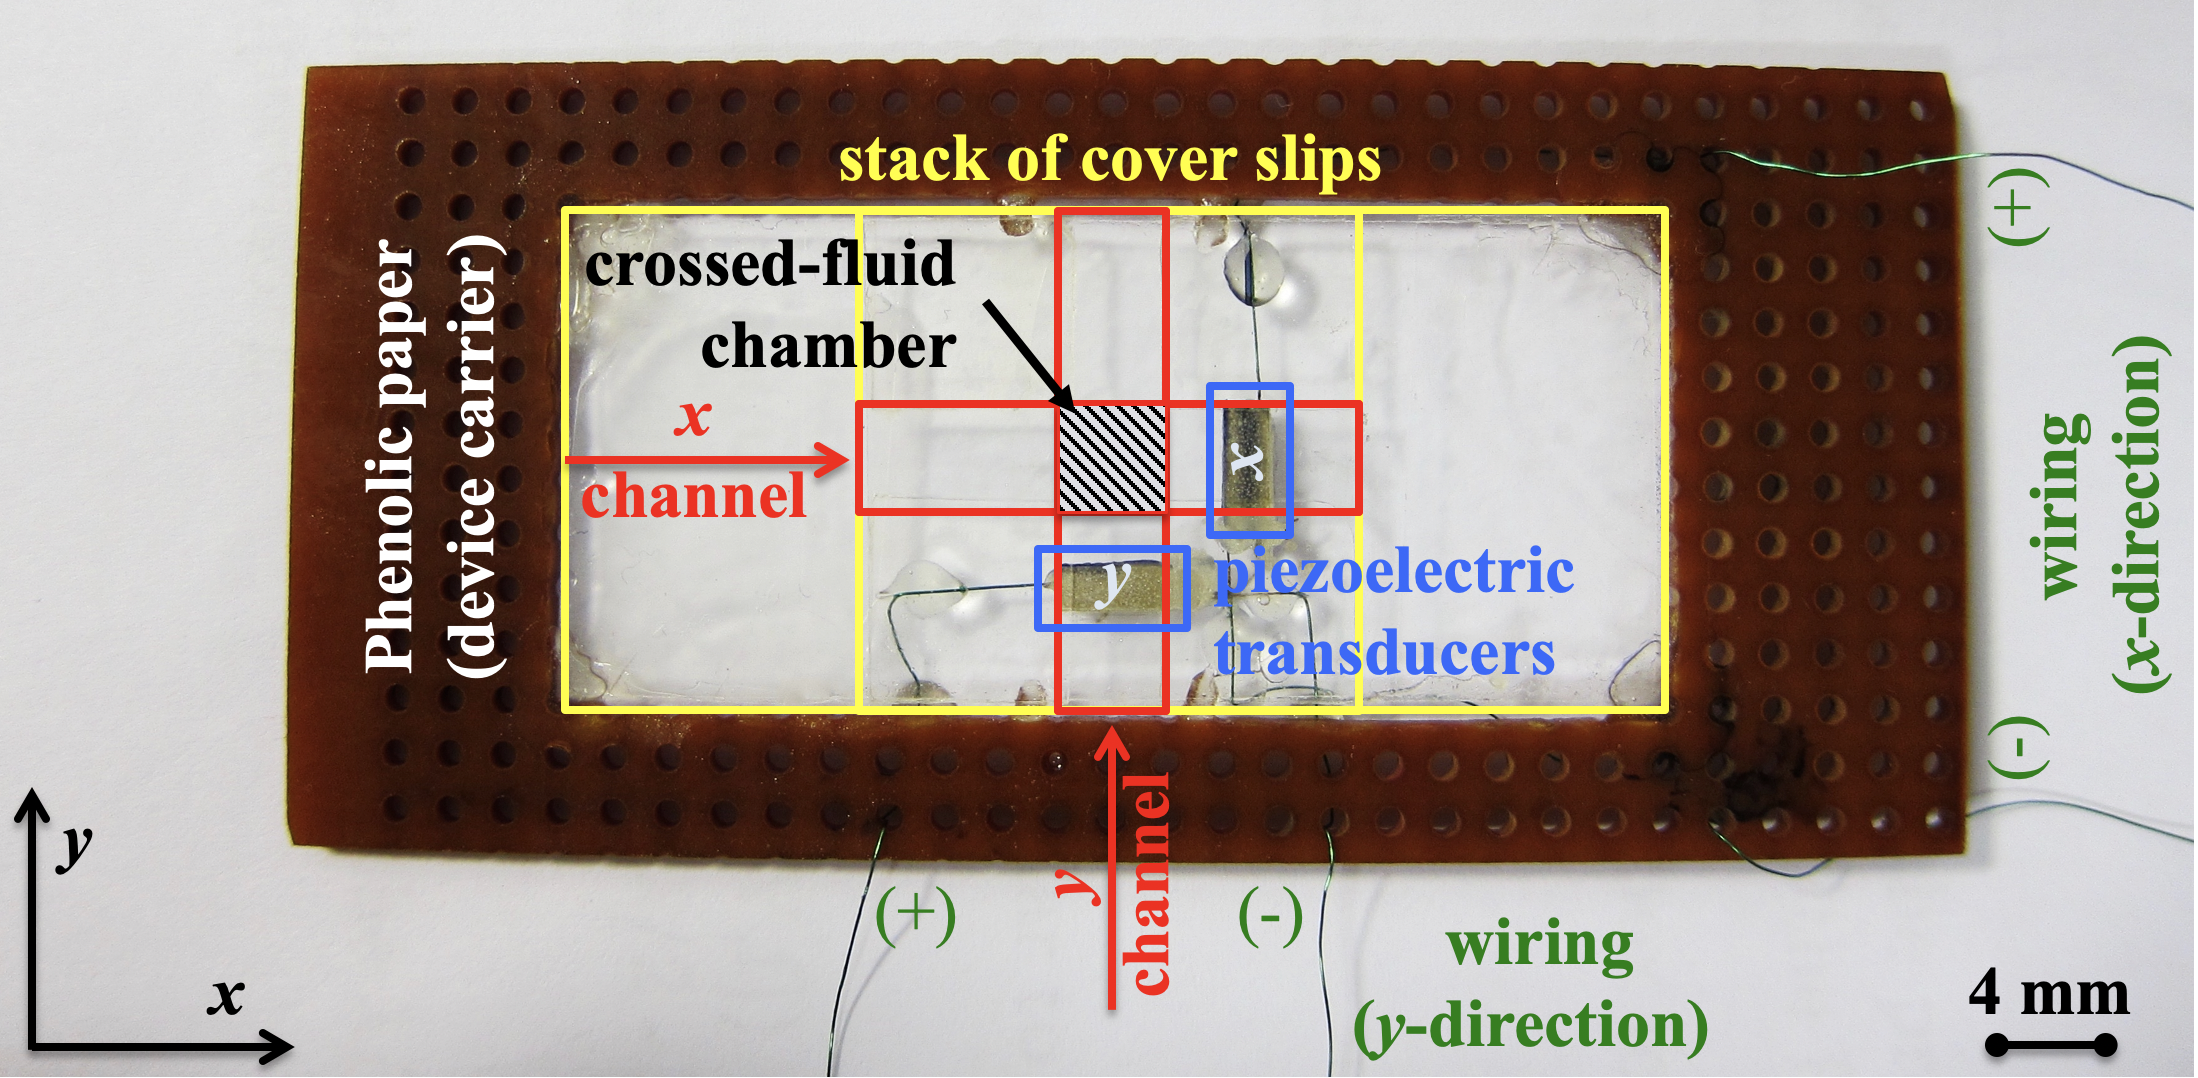
\includegraphics[width=84mm]{\relPath/10_Figures/Fig3.png}
    \caption{Stack of three coverslips form the device where the middle layer 
    includes two fluid channels (\SI{4.0x22}{\mm} with a depth of 
    \numrange{0.13}{0.17} \si{\milli\meter}, red boxes) in an orthogonal 
    arrangement. The two channels intersect and form a \SI{4.0x4.0}{\mm} crossed 
    chamber (black hatched area). Each piezo-electric transducer 
    \SI{4.0x2.0x0.5}{\mm} (PZ26, blue boxes) individually excites a direction.  
    The relative phase difference $\zeta$ of the excitation signals is freely 
    adjustable. The phenolic paper holds the stack and has the size of a 
    standard specimen slide for mounting.\label{fig:VT-Fig3}}
\end{figure}
%%%%%%%%%%%%%%%%%%%

Two piezo-electric transducers (Ferroperm, Pz26, $l$, $w$, and $h$ = \numlist{4; 
2; 1} \si{\mm}, Kvistgaard, Denmark) were glued on the stack of coverslips with 
conductive glue (EPOXY Technology, H20E, Billerica, MA, USA) perpendicular to 
each channel in $x$- and $y$-direction. The distance between the center of the 
fluidic chamber and each transducer was \SI{7}{\mm}. This distance was set such, 
that the microscope objective stays clear from the transducers. The resulting 
thin design of the device ensured the usage of the optical trap and decoupled 
the standing wave modes in the channels ($x$ and $y$). This specific design 
enabled controlled excitation of standing wave modes in the directions of $x$ 
and $y$ as well as an individual control of the excitation phase $\zeta$ (see 
\cref{fig:VT-Fig4}).

For our measurements we always used the same spatial position within the device.  
Hence, the rotation of the particles is always in the same direction for our 
experiments. However, \citeauthor{Lamprecht2015} \cite{Lamprecht2015} 
demonstrated how the rotation direction is dependent on the spatial location and 
the phase $\zeta$ of the two standing waves. In addition, in the supplemental 
material two videos are provided that show the change of rotation direction when 
changing these two parameters.

%%%%%%%%%%%%%%%%%%%
\begin{figure}
    \centering
    \includegraphics[width=84mm]{\relPath/10_Figures/Fig4.png}
    \caption{The device is filled with a water/glycerol (70$\%$/30$\%$) mixture 
    containing \SI{4}{\micro\meter} copolymer particles (Duke Scientific 
    Cooperation, Palo Alto, CA, USA) and it has two identical modes in $x$- and 
    $y$-direction at \SI{1.043}{\mega\hertz}. a) and b) depict the isolated 
    modes at \SI{15}{\Vrms} for the $x$- and $y$-direction, respectively. The 
    resulting measured wavelength $\lambda_{P}$ was approximately 
    \SI{1.4}{\milli\meter} for both directions.\ c) and d) show the particle 
    pattern for the two orthogonal standing waves inside the crossed-fluid 
    chamber at $\zeta= 0$ and $\zeta= \frac{\pi}{2}$, respectively. These 
    observations confirm the assumption of a 2 dimensional orthogonal standing 
    wave field.\label{fig:VT-Fig4}}
\end{figure}
%%%%%%%%%%%%%%%%%%%


\subsection{Particles \label{sec:VT-particles}}
For the visualization experiment in \cref{fig:VT-Fig4} we used \SI{4}{\micro\meter} 
copolymer particles (Duke Scientific Cooperation, Palo Alto, CA, USA). For the 
optical trapping experiments with single particles we used silica particles 
because they are more precise in their dimensions compared to polystyrene 
particles. In addition, they have better interactions
with the acoustical field. Moreover, the results of \citeauthor{Hahn2016} 
\cite{Hahn2016} suggest that in the region of $R \approx \delta$ and ratios of 
$\sfrac{\rho_{\text{s}}}{\rho_{\text{f}}}$ between 2 and 15 result a greater 
magnitude of the acoustic viscous torque results. With the used fluid ($\rho_{f} 
= \SI{1.1}{\gram\per\cubic\centi\meter}$) and our silica particles ($\rho_{s} = 
\SI{2.0}{\gram\per\cubic\centi\meter}$) the ratio 
$\sfrac{\rho_{\text{s}}}{\rho_{\text{f}}} \approx 1.8$.

In order to validate the proposed power spectrum method two sets of validation 
experiments are explained in \cref{sec:VT-rotationDetectionValidation}. For those 
the \SI{4.39}{\micro\meter} particles were modified differently for each 
experiment. We use this size of particles since they are better visible when 
simultaneously measuring the rotation with a camera. There was the need to 
\emph{mark} the spherical \SI{4.39}{\micro\meter} silica particles because a 
reliable rotation measurement with the camera of unmarked spherical particles 
was not possible.

Two methods for marking were used. In both cases the rotation could be easily 
tracked by optical microscopy because the particle size of 
\SI{4.39}{\micro\meter} silica glass micro-spheres (Microparticles
GmbH, Berlin, Germany) is much larger than the optical resolution.
For the set of experiments, silica particles were deformed between two polished 
metal plates by applying a pressure of \SI{1}{\mega\pascal} to achieve a slight 
degree of non-sphericalness (see \cref{fig:VT-Fig5}). For the second set, uncoated 
particles were distributed on a glass specimen slide (MENZEL GmbH, 
Menzel-Glaesser, Braunschweig, Germany) and coated by a Sputter coater (B7340 
Manual Sputter Coater, Van Loenen Instruments, Zaandam, Netherlands) with a gold 
coating (see \cref{fig:VT-Fig6}). After coating, the particles were half-covered 
with a \SIrange{10}{20}{\nano\meter} thick gold layer at their surface 
orientated to the gold electrode. The coating affected the acoustic properties 
not substantially. The particles showed, i.e., same trapping and rotational 
behavior within the acoustical trap. Averted particle surfaces showed a thinner 
gold layer of about \SIrange{0}{10}{\nano\meter}.

\section{Experimental Procedure\label{sec:VT-experimentalProcedure}}

The observed time-averaged spatial off-set of the particles inside the optical 
trap is naturally zero, but the frequency content of the observed particle 
motion includes the thermal energy content of the particle as well as its 
rotational frequency. The angular frequency appears as an additional peak in the 
power spectrum of the rotating particle. In order to validate this detection 
method, particles with a rotational rate of less than \SI{1.66}{\hertz} 
(\SI{100}{\rpm}) were observed by a high-speed camera (HiSpec1 G2 Mono, Fastec, 
San Diego, USA) while also recording their power spectrum.  In the validation 
experiments the transparent device was filled with \SI{4.39}{\micro\meter} 
silica glass micro-spheres suspended in distilled water at a low concentration 
of a few particles per \si{\micro\liter}.  This low particle concentration does 
not effect the ratio $\tilde{\rho} = \sfrac{\rho_{\text{s}}}{\rho_{\text{f}}}$. 
The open channel ends were sealed with silicone oil to ensure a constant fluid 
volume during the measurements.

\subsection{Rotation Detection 
Validation\label{sec:VT-rotationDetectionValidation}}

Two sets of validation experiments were performed: (i) non-spherical particle 
rotation with slightly non-spherical particles; (ii) spherical particle rotation 
with gold covered particles for increased contrast in the video observation 
\cite{Lamprecht2013}. 

According to \citeauthor{Hahn2016} \cite{Hahn2016}, non-spherical objects can 
also be rotated due to the acoustic VT, but here effects of acoustic radiation 
torques may govern or influence their rotations \cite{Wang2012}. A slightly 
non-spherical \SI{4.39}{\micro\meter} silica particle (see \cref{fig:VT-Fig5}) was 
trapped in the optical potential well with \SI{100}{\milli\watt} laser power and 
moved to the reference position ($x,y,z = 0$) in the center of all three 
dimensions of the fluid chamber. The acoustic pressure field is formed by two 
orthogonal standing waves at the same excitation frequency of 
\SI{1090}{\kilo\hertz} and \SI{10.0}{\Vrms} amplitude. The particle was then 
optically moved to the closest resulting pressure node (intersection of two 
pressure nodal lines in $x$- and $y$-direction) with respect to the reference 
position. Positions of the pressure nodes were determined by a previous set of 
experiments.

The phase difference between the acoustic excitation directions $x$- and 
$y$-direction was set to $\zeta=\sfrac{\pi}{2}$, and the non-spherical particle 
rotated counter-clockwise with $\Omega = \SI{1.12}{\hertz}\,(\SI{67}{\rpm})$ 
(arithmetic mean of \SI{0.3}{\hertz} (\SI{18}{\rpm}) and \SI{1.6}{\hertz} 
(\SI{96}{\rpm}); see also \cref{fig:VT-Fig5}). At $\zeta=0$ the particle did not 
rotate because of the stable, non-varying acoustic potential.

%%%%%%%%%%%%%%%%%%%
\begin{figure}
    \centering
    \includegraphics[width=100mm]{\relPath/10_Figures/Fig5.png}
    \caption{Power spectral density and results of the video analysis of a 
      counter-clockwise rotating non-spherical silica particle at 
      \SI{1090}{\kilo\hertz} and \SI{10.0}{\Vrms} with relative phase shift of 
      $\zeta= \sfrac{\pi}{2}$. The 10 times averaged power spectrum of the 
      $y$-signal of the detection unit (QPD) was recorded with a frequency 
      resolution of $\Delta f = \SI{0.1}{\hertz}$ and a sampling rate of 
      \SI{1}{\MS}. Three main peaks were observed at \numlist{0.3; 0.8; 1.6} 
      \si{\hertz}. The frequency peak at \SI{0.8}{\hertz} corresponds to a 
      relative $xy$-motion of the trapped particle, whereas the peaks at 
      \numlist{0.3; 1.6} \si{\hertz} (\numlist{18;96} \si{\rpm}) are related to 
      a non-constant angular rotation $\Omega(\varphi)$ of the particle. The 
      measured results are in correlation with the determined rotational rate by 
      the high-speed video analysis with a frame rate of \SI{100}{\fps}. See the 
      supplemental material for a optically trapped particle rotating 
      sequentially with two velocities due to its imperfect spherical 
  shape.\label{fig:VT-Fig5}}
\end{figure}%
%%%%%%%%%%%%%%%%%%%

In \cref{fig:VT-Fig5}, the average of 10 power spectral density plots is depicted, 
each obtained from a \SI{10}{\second} recording. The frequency resolution is 
$\Delta f=\SI{0.1}{\hertz}$. Three main peaks were observed in the power 
spectrum at \numlist{0.3; 0.8; 1.6} \si{\hertz}, which correlate with the 
frequencies detected by the contemporaneous video detection. We see these peaks 
on both QPDs for the $x-$ and $y$-direction. However for some of the latter 
rotational measurements, the $xy$-motion of the particle adds more peaks 
depending on the major axis of the acoustic displacement. All other peaks are 
related to multiple repetitions of these angular frequencies due to deviations 
of the spherical shape of the particle.  The peak at \SI{0.8}{\hertz} 
corresponds to a relative $xy$-motion of the particle, whereas the peaks at 
\numlist{0.3; 1.6} \si{\hertz} are related to angular frequencies of the 
non-constant rotation $\Omega(\varphi)$ of the particle. The existence of two 
frequency peaks is related to the influence of different acoustic pressures in 
$x$ and $y$-direction because the amplitude were not yet matched for this 
validation.  Hence, the acoustic radiation forces on the particle have different 
magnitudes in $x$ and $y$-direction. So, the distribution of acoustic radiation 
pressure on the particle changes during its rotation and leads to an additional 
orientation dependent acoustic radiation torque.  The influence of acoustic 
radiation forces on particle orientations is a well-known effect for small 
non-spherical particles with $r \ll \lambda$ \cite{Konig1891,Garbin2015}, but 
this experiment shows that this influence is also large enough to influence the 
rotation by the acoustic VT.  Particles with a larger degree of 
non-sphericalness did not even start to rotate in this set of experiments. This 
is in agreement with the predictions of \citeauthor{Hahn2016} \cite{Hahn2016}, 
that the acoustic VT decreases with a higher degree of elliptical shape of the 
particles. In contrast, the acoustic radiation torque increases and hinders a 
constant rotation of the particle, if the symmetry of the experimental acoustic 
potential at $\zeta= \sfrac{\pi}{2}$ is imperfect.

Previously, optical traps formed by a linearly polarized laser have been applied 
to rotate anisotropic particles \cite{GutirezMedina2010}. However, this torque 
is dependent on the orientation of the anisotropic particle with respect to the 
polarization plane of the laser. If the laser power is high enough, the 
acoustically induced rotation can be inhibited because the anisotropic particle 
is optically locked to the polarization plane. For perfectly spherical particles 
without any shape anisotropy this optical torque vanishes 
\cite{Manzo2006,Friese1998}. We did not observe influences of optical forces on 
the final rotational velocities of the spherical particles because the 
determined velocities in the experiments were independent of the applied laser 
power. For our validation experiments with deformed and gold coated particles we 
did not investigate further the influence of the linearly polarized laser on the 
particles. This indicates that the applied acoustic torque was greater in 
magnitude than the optical torque.

Also, the experiments that are presented afterward show that the particle 
rotation is dominated by the acoustic field. By moving the particle through the 
flow cell or by changing the phase of the excitation signal, the rotation can be 
stopped, started and reversed (see \cref{fig:VT-Fig8} and the video in the 
supplemental material).

A closer investigation was not possible in our current experimental set-up 
because particles sank due to gravity if the laser was turned off. Observed 
rotations near fluid boundaries (bottom plate) are governed by influences of 
near-boundary effects, e.g.\ higher viscous drag, different acoustic scattering 
and streaming which would complicate an investigation of low laser powers on the 
particle rotation.

The second set of validation experiments employed spherical particles with a 
thin gold layer to increase the contrast for the video observation 
\cite{Lamprecht2013}. The additional gold layer changed the optical properties of 
the particles and led to a different optical trapping behavior in the 
experiments. Most of the particles could not be trapped optically because the 
gold layer reflected the incident laser light (\SI{785}{\nano\meter}) and the 
resulting optical scattering forces pushed the particles away from the laser 
focus \cite{Zhou2020,Ashkin1992,Svoboda1994}. The particle needs to be 
transparent for the wavelength of the laser, in order to enable trapping. 
However, due to statistical variations of the coating process some particles 
were optically trappable, since just a small portion of the surface was coated.  
And hence, just a small portion of the incoming laser was reflected. One example 
of an optically trapped particle with a constant and stable rotation is shown in 
\cref{fig:VT-Fig6}. The brighter regions at the surface of the particle arise from 
the reflected laser light due to the partial gold coating.  These regions 
rotated with the optically trapped particle due to the acoustic VT.\@ The 
angular change of reflected light on the particle surface was then determined by 
the QPDs of the optical detection unit and increased the signal strength by a 
factor of 100 with respect to uncoated particles. The recorded power spectrum of 
the $x$- and $y$-signals included the information about the angular frequency of 
the rotating particle.

An example for a recorded power spectrum of a rotating gold-layered 
\SI{4.39}{\micro\meter} silica particle at an acoustic excitation frequency of 
\SI{1090}{\kilo\hertz} and amplitude of \SI{2.5}{\Vrms} with a relative phase 
shift of $\zeta= \sfrac{\pi}{2}$ is depicted in \cref{fig:VT-Fig6}. A clear peak 
can be seen at \SI{1.3}{\hertz}. The determined rotational rate of the particle 
by video observations was \SI{1.31}{\hertz} (\SI{78.6}{\rpm}), which correlates 
with the measured peak at \SI{1.3}{\hertz} (\SI{78.0}{\rpm}).  A further 
variation of the acoustic excitation parameters (amplitude and relative phase) 
shifted the peaks in frequency as predicted by 
\cref{eq:VT-Eq1,eq:VT-AcGovEqConti} (results are not shown) 
\cite{Lamprecht2013}.

%%%%%%%%%%%%%%%%%%%
\begin{figure}
    \centering
    \includegraphics[width=100mm]{\relPath/10_Figures/Fig6.png}
    \caption{Power spectral density and results of the video analysis of a 
      counter-clockwise rotating gold-coated spherical \SI{4.39}{\micro\meter} 
      silica particle at \SI{1090}{\kilo\hertz} and \SI{2.5}{\Vrms} with 
      relative phase shift $\zeta= \sfrac{\pi}{2}$. The 10 times averaged power 
      spectrum of the $y$-signal of the detection unit (QPD) was recorded with a 
      frequency resolution of $\Delta f=\SI{0.1}{\hertz}$ and a sampling rate of 
      \SI{1}{\MS}. A clear peak at \SI{1.3}{\hertz} and two additional peaks at 
      \numlist{2.6; 3.9} \si{\hertz} were observed. The amplitudes of the 
      additional peaks were one order of magnitude smaller as the amplitude of 
      the peak at \SI{1.3}{\hertz}. The peak at \SI{1.3}{\hertz} correlates with 
  the determined rotational rate by the high-speed video analysis at a frame 
  rate of \SI{100}{\fps}.\label{fig:VT-Fig6}}
\end{figure}%
%%%%%%%%%%%%%%%%%%%

\subsection{Rotation of particles where $\normBdLayer \approx 
1$\label{sec:VT-rotationParticles}}

The determinations of the rotational rate with the power spectrum-method opened 
the possibility to measure fast rotations ($>\SI{25}{\hertz}$ (\SI{1500}{\rpm})) 
of particles with a radius $R$ about \SI{1}{\micro\meter}.  For such small 
particles the ratio of the thickness of the viscous boundary layer $\delta$ and 
the particle radius $R$ approaches 1 ($\normBdLayer \approx 1$) in the 
\si{\mega\hertz}-range (\SIrange{1}{10}{\mega\hertz}). The analytical formulas 
become invalid for the case that $\normBdLayer > \sfrac{1}{15}$ \cite{Hahn2016}.  
Particle rotations within the limit $\normBdLayer \approx 1$ were experimentally 
validated by an investigation of silica spheres with a \SI{2.06}{\micro\meter} 
(Microparticles GmbH, Berlin, Germany) diameter resuspended with a 
water/glycerol (70$\%$/30$\%$) mixture.  The viscosity $\mu_f$ of the aqueous 
glycerol solution was \SI{0.06}{\pascal\second} \cite{Jerome1968} with a 
determined density of \SI{1.1}{\gram\per\centi\meter\cubed} (dense knife, DMA 
35N, Anton Paar GmbH, Graz, Austria) and increased the thickness of the viscous 
boundary layer to approximately \SI{1.33}{\micro\meter} at an excitation 
frequency of \SI{1043}{\kilo\hertz} ($\lambda \approx \SI{1.4}{\mm}$). The 
normalized viscous boundary layer is therefore $\normBdLayer \approx 1.30$.

The optical trapping set-up was originally designed to measure the acoustic 
force and pressure amplitudes inside micro-fluidic channels and cavities 
\cite{Lakaemper2015,Lamprecht2016}. The same procedure was used here to measure 
the local acoustic pressure amplitudes inside the fluid chamber of the 
transparent micro-device. An accurate prediction of the acoustic pressure 
amplitudes $A_{X}$ and $A_{Y}$ of the two orthogonal standing waves was 
important to determine the strength of the acoustic VT by observing the 
steady-state rotational rate $\finalOmega$ of rotating particles.

Therefore, the local acoustic pressure amplitudes $A_{X}$ and $A_{Y}$ were 
individually measured in $x$- and $y$-direction by exciting only one transducer 
of the corresponding $x$- or $y$-direction, respectively. We measured the 
acoustic forces in all three dimensions ($x$, $y$, $z$) acting on the 
\SI{2.06}{\micro\meter}-particle inside the optical trapping potential. The 
spatial measurement range was $\pm \SI{0.55}{mm}$ in the $x$- and $y$-direction.  
The point $(\SI{0.21}{\mm}, \SI{0.22}{\mm})$, measured relatively to the middle 
of the fluid chamber, corresponded to the spatial position where a pressure 
nodal line in $x$- and $y$-direction overlapped.

The maximal force amplitudes at \SI{1043}{\kilo\hertz} were 
\SIrange{-96}{+25}{\femto\newton} for the $x$-direction and 
\SIrange{-32}{28}{\femto\newton} for the $y$-direction. The peak-to-peak value 
of the determined forces in $y$-direction was about two times weaker than in 
$x$-direction. This factor of 2 was used to calibrate the piezoelectric 
excitation amplitude to reach equal acoustic pressure amplitudes in both 
excitation directions.

The excitation amplitude $U_{el}$ is proportional with the acoustic pressure 
amplitude $A_{x,y}$ ($U_{el} \propto A_{x,y}$), whereas the acoustic radiation 
force $F_{ac}$ has a quadratic dependency of the acoustic pressure amplitudes 
$A_{x,y}$ ($F_{ac} \propto A_{x,y}^2$) \cite{Barnkob2010}. Therefore, the 
excitation amplitude of the piezoelectric transducer in $y$-direction was 
increased by a factor of $\sqrt{2}$ for all further investigations. The acoustic 
pressure amplitude $p_{a}$ was calculated via
%%%%%%%%%%%%%%%%%%%
\begin{equation}
\label{eq:VT-PressurePredictions}
p_{a}^{2} = \frac{F}{\pi\,R^{3}\,\kappa_{0}\,\Phi(f_{1},f_{2})} 
\frac{1}{k\,\sin(2k\,x)} =
\frac{F}{\pi\,R^{3}\,\kappa_{0}\,\Phi(f_{1},f_{2})} 
\frac{\lambda_{\text{p}}}{2\pi\,\sin(x\,\sfrac{4\pi}{\lambda_{\text{p}}})}
\end{equation}
%%%%%%%%%%%%%%%%%%%
where a 1-dimensional standing plane wave is assumed \cite{Settnes2012a}. $F$ is 
the force measured with the optical trap, $\lambda_{\text{p}}$ the wavelength of 
the pressure field, $k = \sfrac{2\pi}{\lambda_{\text{p}}}$ the wavenumber, $R$ 
the radius of the spherical particle, $\kappa_{0}$ the compressibility of the 
fluid, $\Phi(f_{1},f_{2})$ the so-called acoustic contrast factor, and 
$\sin(kx)$ the spatial dependency of the standing wave.  Since the force was 
measured at the force maximum $\sin(2\,kx)$ is set to $\sin(\sfrac{\pi}{2}) = 
1$. In addition, because of the value for the normalized viscous boundary layer 
$\normBdLayer \approx 1$, the corrected dipole factor  
$f_{2}(\tilde{\rho},\normBdLayer)$ of \citeauthor{Settnes2012} 
\cite{Settnes2012} was utilized. With this, the determined acoustic pressure 
amplitude for the standing wave in $x$-direction was \SI{245}{\kilo\pascal} for 
the measured acoustic forces and wavelength if an influence of acoustic 
streaming was neglected. 

After the calibration of the excitation amplitudes and the acoustic pressures of 
both acoustofluidic channels the acoustic VT was quantitatively investigated 
inside the fluid chamber. One \SI{2.06}{\micro\meter} silica particle was 
optically trapped and moved in $x$-direction inside the wave field of two 
orthogonal standing waves, while measuring its power spectrum at specified 
measurements points. The location of one specific pressure nodal line for an one 
dimensional standing wave in $x$- and $y$-direction at \SI{1043}{\kilo\hertz} 
was determined at $x=\SI{0.21}{\mm}$ and $y=\SI{0.22}{\mm}$, respectively. These 
nodal lines formed a local pressure node at their intersection if the acoustic 
excitation was shifted in phase with $\zeta = \sfrac{\pi}{2}$. There, the 
acoustic VT had its maximum value. Therefore, a measurement line in 
$x$-direction was defined between $x=0.20\pm0.55~\si{\milli\meter}$ at constant 
$y=\SI{0.22}{\milli\meter}$.

The particle exerted a counter-clockwise rotation at the local pressure node due 
to the acoustic VT at \SI{1043}{\kilo\hertz} with \SI{10.0}{\Vrms} and 
\SI{14.2}{\Vrms} excitation amplitude in $x$- and $y$-direction, respectively.

The detection of the angular frequency in a recorded power spectrum was not 
trivial for those small and spherical silica particles due to their low 
signal-to-noise ratios. Additionally, the power spectrum was disturbed by added 
frequencies of the acoustic excitation set-up; namely, an additional peak at 
\SI{100}{\hertz} originating from the voltage supply and \SI{170}{\hertz} from 
the amplifier itself.  Therefore, all measurements were repeated with a 
ten-times lower excitation amplitudes in $x$- and $y$-direction to calibrate the 
power spectrum measurements due to unknown influences of the environment and 
attached set-ups. An initialization of particle rotations was not observed at 
these low excitation amplitudes. A peak detection algorithm (implemented in 
MatLab) used the calibration measurement to eliminate disturbances on the 
determined power spectrum of a locally rotating particle due to VT.\@

\Cref{fig:VT-Fig8} depicts the power spectrum of a rotating particle with a clear 
peak at a frequency of \SI{165}{\hertz}. The particle was located at the 
relative location (-0.075, 0.220) \si{\mm} and its rotation was initialized at 
\SI{1043}{\kilo\hertz} with an excitation amplitude of \SI{10.0}{\Vrms} and 
\SI{14.2}{\Vrms} in $x$- and $y$-direction, respectively.  An appearance of 
additional peaks at a multiple of the angular frequency was not monitored by the 
peak-detection algorithm, likely because the amplitude of these peaks was below 
the noise floor. Their signal strength was expected to be one order of 
magnitude smaller (see \cref{fig:VT-Fig5,fig:VT-Fig6}).  The detection 
algorithm had a threshold value of 3 (signal-to-noise ratio) for indicating 
peaks in determined power spectrum.  \cref{fig:VT-Fig8}b depicts the 
corresponding calibration power spectrum of \cref{fig:VT-Fig8}a.

\Cref{fig:VT-Fig10} depicts the peaks detected by the peak-detection algorithm. 
Each point represents a separate rotational rate measurement. Interestingly, the 
strength of the angular frequency peaks was proportional to Brownian noise with 
$\sfrac{1}{f^2}$. These peaks are due to the particle rotations at positions 
within the spatial range of $x=0.21\pm\SI{0.55}{\mm}$ and $y=\SI{0.22}{\mm}$.  
The spatial dependency and formation of these peaks were in correlation with 
\cref{eq:VT-Eq1} and the maximal frequency $f$ of a peak in the power spectrum was 
\SI{229}{\hertz} ($ \finalOmega = \SI{13.8e3}{\rpm} $). The quantitative 
analysis revealed that maximal rotation appeared at $x=\SI{0.16}{\mm}$ (pressure 
node) and the resulting acoustic wavelength in $x$-direction was \SI{1.9}{\mm}.  
A one-dimensional wave in water at $f=\SI{1043}{\kilo\hertz}$ predicts an 
acoustic wavelength of $\lambda = \sfrac{c}{f} \approx \SI{1.4}{\mm}$ (compare 
\cref{fig:VT-Fig4}). The difference in wavelength from \cref{fig:VT-Fig4} 
($\lambda \approx \SI{1.4}{\mm} $) to the fitted value of $\lambda \approx 
\SI{1.9}{\mm} $ may be related to an off-set in orientation of the 
3-dimensional wavenumber $|\bm{k}|^{2} = k^{2}_{x} + k^{2}_{y} + k^{2}_{z}$ in 
the optical trapping set-up. Eigenfrequencies and their acoustic fields are 
influenced by the optical trapping set-up due to the additional interface 
between the acoustofluidic device and the water-immersion objective 
\cite{Lamprecht2016}.  \Cref{fig:VT-Fig4} was observed with a standard 
microscope lens that did not need to have an immersion oil layer on top of the 
device.

%%%%%%%%%%%%%%%%%%%
\begin{figure}
    \centering
    \includegraphics[width=100mm]{\relPath/10_Figures/Fig9.png}
    \caption{a) Measured power spectrum of an optically trapped 
    \SI{2.06}{\micro\meter} particle that rotated counter-clockwise due to the 
    acoustic VT at \SI{1043}{\kilo\hertz} with \SI{10.0}{\Vrms} and 
    \SI{14.2}{\Vrms} excitation amplitude in $x$- and $y$-direction, 
    respectively. The particle was located at (-0.075, 0.220) \si{\mm}. The 
    spectrum of the $x$-signal (QPD) was recorded and 10 times averaged with a 
    frequency resolution of $\Delta f=\SI{1}{\hertz}$ and a sampling rate of 
    \SI{1}{\MS}. A clear signal peak due to particle rotation at 
  \SI{165}{\hertz} was observed with a signal-to-noise ratio of about 5. The 
signal peak at \SI{110}{\hertz} is related to influences of the acoustic 
excitation set-up.\ b) Control measurement of a non-rotating optically trapped 
\SI{2.06}{\micro\meter} particle under acoustic excitation at 
\SI{1043}{\kilo\hertz} with \SI{1}{\Vrms} and \SI{1.42}{\Vrms} excitation 
amplitude in $x$- and $y$-direction, respectively. A particle rotation was not 
initialized at these low excitation amplitudes and these recorded power spectrum 
of non-rotating \si{\micro\meter} particles were used to identify the peaks not 
related to particle rotation power spectrum due to influences of the environment 
and the acoustic excitation set-up. The peak at \SI{110}{\hertz} is related to 
amplifier noise and vanished when the acoustic excitation set-up was turned off 
\cite{Lamprecht2016}.\label{fig:VT-Fig8}}
\end{figure}
%%%%%%%%%%%%%%%%%%%

%%%%%%%%%%%%%%%%%%%
\tikzsetnextfilename{VT_results}
\begin{figure}[tb]
  \centering
  \includegraphics[]{Plots/cache/VT_results.eps}
    % \begin{tikzpicture}
    %     \begin{axis}
    %         [scale only axis,
    %         width = 89mm,
    %         height = 5cm,
    %         xtick = {-0.5,-0.25,0,0.25,0.5},
    %         xmin = -0.55, xmax = 0.55,
    %         ymax = 280, ymin = -5,
    %         xlabel = {Realative x position [\si{\mm}]},
    %         ylabel = {power spectrum Peak Frequency [\si{\hertz}]}]

    %         \addplot[red,thick,mark size=4pt,only marks,mark=x] table[x=y, 
    %         y=f,col sep=comma] {\relPath/40_Fitting/datapoints.dat};

    %         \addplot[thick,blue,dashed] table[x=y, y=f,col sep=comma] 
    %         {\relPath/40_Fitting/datapointsFit.dat};

    %         \node[blue,above] at (axis cs: 0.16,229) 
    %         {$\left|229.18\,\sin\left(3.30\,X_{i} + 1.03 \right)\right|$};

    %     \end{axis}
    % \end{tikzpicture}
    \caption{Spatial dependency of frequency peaks (red) due to the acoustic VT 
      from the power spectrum-method. Multiple power spectra of a 
      \SI{2.06}{\micro\meter} silica particle were recorded at specific 
      measurement points in $x$-direction at $x=\SI{0.21}{\mm}\pm\SI{0.5}{\mm}$ 
      and $y=\SI{0.22}{\mm}$. The acoustic field formed two orthogonal standing 
      waves in $x$- and $y$-direction at \SI{1043}{\kilo\hertz} with a relative 
      phase shift of $\zeta =\frac{\pi}{2}$. The determined frequency peaks were 
      fitted to the equation $\left|c_{1}\,\sin(c_2\,X_i + c_3)\right|$ (dashed 
      blue).  The resulting maximal frequency $f$  from the fit was 
      \SI{229}{\hertz} ($ \finalOmega = \SI{13.8e3}{\rpm}$) and the determined 
      acoustic wave in $x$-direction $\lambda_{X}=\sfrac{2\pi}{c_2}$ was 
    \SI{1.90}{\mm}. The pressure nodal point with maximal rotational rate was 
  determined at $x=\SI{0.16}{\mm}$, whereas zero VT was determined at 
$x=\SI{-0.31}{\mm}$ (pressure anti-node).\label{fig:VT-Fig10}}
\end{figure}
%%%%%%%%%%%%%%%%%%%

\section{Conclusion\label{sec:VT-conclusion}}

The combination of an optical trap and a transparent VT device opened the 
possibility to measure the VT independently of the acoustic radiation force. The 
power spectrum analysis provided the quantitative information about the angular 
frequency $\Omega$. Unwanted effects related to close proximities of walls near 
the rotating particle and influences of oscillating micro gas bubbles were 
avoided.  The optically levitated particle ensured a largely unaffected rotation 
due to the acoustic VT.\@ 

Moving the stage of the optical set-up changed the rotation direction of a 
trapped and rotated particle between two neighboring pressure nodes because of 
the acoustic VT \cite{Lamprecht2015} (see the supplemental material for a 
particle rotation in different directions depending on the spatial location 
inside the wave field).  These kinds of experiments were so far unattainable in 
a continuous manner and for unstable acoustic particle positions (positive 
acoustic contrast factor) of zero VT.\@

The validation experiments showed that the detected additional peaks in the 
measured power spectrum are directly related to the rotational rate of the 
particle rotation. The detected signals had peaks at multiples of this peak 
frequency.  However, for transparent silica particles with an almost perfectly 
spherical shape the amplitudes of the multiples were too small to overcome the 
signal-to-noise-ratio. The high-speed video analysis is limited by the camera's 
frame rate. In contrast, the detection bandwidth of the optical trap easily 
spans tens of \si{\kilo\hertz}. As already mentioned, optical trapping has some 
unique advantages to investigate the acoustic VT: 1) Allows to probe almost  any 
spatial position within the acoustofluidic device. 2) Measures rotational 
frequencies up to multiple \si{\kilo\hertz}. 3) Works with conventional, non 
coated, spherical particles. 4) Frequencies are directly visible in the data (no 
need for post processing of video data).

In order to calculate the theoretical rotational rate $\finalOmega$ of the 
particle, the local acoustic pressure amplitude needs to be known in advance.  
Because of that, a local acoustic pressure amplitude analysis was carried out 
before the rotation detection experiments. Depending on the calculation 
approach, different results are obtained for the rotational rate. The analytical 
calculation for the final rotational rate $\finalOmega$ (see \cref{eq:VT-Eq1}) 
\cite{Lamprecht2015, Busse1981, Rudnick1977, Wang1989} with a dynamic fluid viscosity of 
$\mu_{f} = \SI{0.06}{\pascal\second}$ led to rates between 
\SIrange{613}{811}{\hertz} (\SIrange{36.8e3}{48.7e3}{\rpm}). The numerical 
calculations of \citeauthor{Hahn2016} \cite{Hahn2016} yield a final rotational 
rate for a \SI{2.06}{\micro\meter} silica particle with $\normBdLayer=1.30$ of 
\SIrange{208}{277}{\hertz} (\SIrange{12.5e3}{16.6e3}{\rpm}) at room temperature 
(\SI{25}{\celsius}).  The first value for the rotational rate corresponds each 
time to the theoretical wavelength of $\lambda \approx \SI{1.4}{\mm}$ (see 
\cref{fig:VT-Fig4}) and acoustic pressure amplitude $p_{a}\left(\lambda\right) = 
\SI{245}{\kilo\pascal} $; the latter to the measured $\lambda \approx 
\SI{1.9}{\mm}$ (see \cref{fig:VT-Fig10}) and $p_{a}\left(\lambda\right) = 
\SI{282}{\kilo\pascal} $. The disagreement between our experiments and 
\cref{eq:VT-Eq1} is regarding the equilibrium state for the final rotational rate 
$\finalOmega$. The spatial dependency of \cref{eq:VT-Eq1} ($\cos\left(k\,X\right), 
\cos\left( k\,Y \right)$) agrees with our experiments.

In contrast to that, the power spectrum-method estimates the steady-state 
rotational rate $\finalOmega$ to \SI{229}{\hertz} (\SI{13.8e3}{\rpm}). This 
value is very close to the numerically obtained values (about 10$\%$ higher for 
$\lambda \approx \SI{1.4}{\mm}$ or 17$\%$ lower for $\lambda \approx 
\SI{1.9}{\mm}$).  These deviations can be in part explained by a decrease of 
the fluid viscosity due to laser-induced heating (up to \SI{2}{\kelvin}) in 
close proximity of the laser focus \cite{Peterman2003}. Since the measured force 
of our trap scales with $\sqrt{\mu}$ and the viscosity variation around 
\SI{25}{\celsius} is relatively small, the temperature induced measurement 
errors are about 2\%.  This slightly changes the acoustic pressure amplitudes 
with respect to the calibrated pressure of \SI{245}{\kilo\pascal} ($\lambda 
\approx \SI{1.4}{\mm}$) or \SI{282}{\kilo\pascal} ($\lambda \approx 
\SI{1.9}{\mm}$) because the investigated pressure node was located slightly off 
the calibration lines.  Also, the in oil immersed lens of the optical trap 
changes the theoretical (pure) 1-dimensional acoustic field to a 3-dimensional.

The experiment clearly showed that the analytical calculations of 
\citeauthor{Lamprecht2015,Busse1981, Rudnick1977, Wang1989} \cite{Lamprecht2015, Busse1981, 
Rudnick1977, Wang1989}  overestimate the rotational velocities at ratios $\normBdLayer 
\approx 1$. Furthermore, the complexity and spatially varying torques on 
\si{\micro\meter} particles were measured, whereas the simulations are limited 
to the ideal case of plane-standing waves and incompressible particles in an 
infinitely large fluid domain. 

A further application of the acoustic torque analysis with an optical trap could 
be the experimental determination of the influence of the particle density on 
the acoustic VT.\@ Particles with the same density can show different rotational 
directions at a fixed point in the acoustic field, if the ratio $\normBdLayer$ 
changes \cite{Hahn2016}.

Optical torques on double refracting quartz particles is a possible tool to 
directly measure acoustic torques \cite{La2004}. The laser power of such 
modulated optical traps could be used to calibrate acoustic torques on trapped 
particles at equilibriums where the optical torque counteracts the acoustic 
torque. 

% \vspace*{7mm}

% A.L and C.G. contributed equally to this work.



% \cleardoublepage
% \chapter[Discussion \& Outlook]{Discussion and Outlook}\label{ch:discussion}

\section{Discussion}
In this thesis we presented the application of the fast position readout of a 
trapped spherical particle within our optical trapping (OT) setup to two micro 
scale Acoustofluidics (MSAF) phenomena: 1) the transient build up behaviour of 
acoustic streaming (AS) as well as of the acoustic radiation force (ARF); 2) 
the viscous torque induced rotation of spherical particles in a viscous fluid 
where the viscous boundary layer (VBL) is as large as the particle radius 
itself $\delta \approx R$.

The investigations of both phenomena are possible because the laser beam 
causing the trapping potential carries positional information about the 
particle's relative position to the laser focal point. In order to extract this 
information from the laser beam, the beam must be collimated after the trapping 
and focused onto photo detectors. For the resolution of two orthogonal 
directions of the in-plane movement, the photo detector (PD) must be a quadrant 
photo detector (QPD). For the axial movement a single PD is sufficient because 
only the total intensity onto the PD is needed.

The physical unit of the (Q)PDs output is \si{\volt}. In order to convert the 
voltage to the unit of \si{\meter}, we take advantage of the linear regime of 
(Q)PDs where a change in measured voltage is proportional to the movement of 
the particle within the trap. In this regime, the OT can also be used as force 
measurement device because it has the same properties as a linear mechanical 
spring. The respective start and end point of this regime is dependent on a 
multitude of parameters. Movements of less than \SI{100}{\nm} are still linear 
for our OT setup. The voltage-conversion factor as well as the stiffness of the 
OT can be derived from the single-sided frequency spectrum of the trapped 
particle. The particles in the fluid suspended are so lightweight and small 
that they undergo visible Brownian motion. Brownian motion is a random process 
with the property that over a long time period the particle will be back at its 
initial position. Also while being trapped the particle undergoes Brownian 
motion. The frequency content of a trapped particle in any spatial direction 
follows the curve of a low-pass filter. With the amplitude at zero frequency 
$A_{0}$ and the cutoff frequency $f_{\MR{c}}$ where 
$A\vert_{f=f_{\MR{c}}}=\sfrac{A_{0}}{2}$ it is possible to calculate the 
voltage-meter conversion factor as well as the stiffness for each spatial 
direction separately.

Besides the size of the trapped particle the conversion factor is dependent on 
the viscosity of the surrounding fluid. Exact knowledge of the viscosity is 
unavoidable for quantitatively precise measurements. The viscosity of the fluid 
is in general a function of its temperature. While the ambient temperature is 
straightforward to measure, the measurement of the temperature within a MSAF 
device or at the focal point of the trapping laser is cumbersome. Although the 
intensity of our laser exceeds the sun's intensity by orders of magnitudes, we 
showed in \cref{sec:TO-temperature} that for our setup the laser induced 
temperature change and therefore the temperature induced viscosity change is 
negligible for all our experiments. However, this is not true for every OT 
because the temperature change does not only depend on the laser power itself 
but even more on the laser wavelength-fluid combination, and therefore the 
absorption at a specific wavelength.

To investigate the first MSAF phenomena, we develop a new measurement method in 
\cref{ch:timeconstant} to visualize the transient build up of the ARF and AS 
and then study in \cref{ch:pulsing} the effects of a pulsed excitation on the 
respective build up times. Key for those experiments is, that the ARF and AS 
induced particle displacement are along orthogonal spatial direction. Moreover, 
the ARF displacement is along one of the axes of the in-plane QPD and the AS 
displacement is along the axial direction on another QPD. Hence, the measured 
displacement data is also separated and cross-talk free. We validated the 
orthogonality of the ARF and the drag force from AS by steady state force 
measurements with two different sized particles where all experimental 
parameters besides the particle radius were kept the same. The drag force from 
AS scales with the particle radius, $\FAS\propto R$ and the ARF with the volume 
of the particle, $\FARF\propto R^{3}$. The ratio of the measured forces along 
same directions but of different particle sizes showed the same scaling laws. 

However, without modifications on the OT we are not able to measure any of 
those effects because the timeconstant of the OT $\tOT$ is much larger than the 
theoretical build up time of the ARF. In fact, for our set of experimental 
parameters and our device configuration $\tOT \approx \tas \gg \tarf$ with 
$\tas = \SI{1.59}{\ms}$ and $\tarf = \SI{1.4}{\us}$, respectively. We reduced 
$\tOT$ effectively to zero by reducing the laser power to almost zero such that 
there is no effective trapping by the OT. The laser cannot be switched off 
completely because the beam is the cause for the measured intensity at any of 
the (Q)PDs.

Because of the laser power reduction, we also needed to install an optical 
shutter right before the (Q)PDs. The laser intensity is too high for the photo 
detectors. In normal trapping mode a set of filters reduces the intensity to 
less than 0.01\% of the incoming intensity. The optical filter is actuated to 
be almost completely closed such that it acts as intensity filter if the laser 
power is high (trapping) and opens as soon as the laser power is reduced for 
the measurement itself.

The laser power change occurs almost instantaneously but the shutter has an 
opening time of less than \SI{15}{\ms}. To ensure undisturbed data we wait 
\SI{25}{\ms} before starting the acoustic excitation. During this time the 
particle will start to sediment due to gravity because it is not trapped stably 
anymore. However, this movement is only $\approx 0.05\,R$ along the direction 
of the laser beam and, hence, does not hinder the measurement; the in-plane 
movement is zero because no forces besides gravity are acting on the particle.

The (pulsed) acoustic excitation is then switched on for only \SI{30}{\ms} 
because a longer excitation would lead to such large displacements -- primarily 
along the ARF direction -- that the same particle could not be re-trapped by 
the OT. For our studies we were not interested in the actual displacements but 
in the time it takes until the movement along any direction starts. For actual 
displacement magnitudes one would need to retrieve the voltage-meter conversion 
factor but for that the particle needs to be trapped. Hence, only the voltage 
at the (Q)PDs can be investigated.

Because the particle is free-floating and, therefore, uncontrolled in its 
location for the first \SI{25}{\ms} we repeat the measurement multiple times 
per location and average the measured data. To further subtract the gravity 
induced movement from the data we perform the same amount of measurements with 
no acoustics at all and then subtract the averaged \emph{no-acoustic} data from 
the \emph{acoustics} data.

The data for both types of experiments (non-pulsed and pulsed) showed that the 
ARF induced displacement starts immediately whereas the AS induced displacement 
takes significantly longer. The measured time offset between ARF and AS is an 
explanation why in experiments~\cite{Castro2016,Hoyos2013} a pulsed acoustic 
excitation suppresses the build up of AS whereas numerical 
investigations~\cite{Muller2015} with an ideal fluid cavity reveal a much 
smaller offset which does not suppress streaming. Although the data has the 
unit of \si{\volt} and not \si{\meter}, the slope of the AS and ARF induced 
displacement is showing that the acceleration after the build up by any of two 
effects occurs fast and then transitions into constant velocity (linear slope). 
A constant velocity implies a constant force acting on the particle.
% It is a valid statement because the measured voltage (within the linear regime 
% of the (Q)PDs) is the displacement divided by the voltage-meter conversion 
% factor. The slope of the voltage-over-time data equals the slope of the 
% displacement which is in turn the velocity of the particle.

Additionally, the pulsed excitation measurements revealed that a pulsed 
excitation leads to a greater reduction in terms of the final displacement at 
the end of the measurement on the AS than it does on the ARF. We measure this 
observation for all pulsing frequencies. The ARF and AS are linearly dependent 
on the acoustic energy density within the fluid cavity. All our data also 
showed this relation but with a steeper slope for AS than the ARF. The pulsed 
excitation results help to further explain the experimental shown suppression 
of AS~\cite{Hoyos2013,Castro2016}. However, with our measurement protocol we 
can only measure for the first \SI{30}{\ms} of acoustic excitation, and any 
MSAF application is operated continuously where all fields have developed 
fully. At the moment, we cannot measure these effects during steady-state.


Compared to the first phenomena, no setup modifications at the OT are necessary 
for the second MSAF phenomena: the rotational speed measurement of a spherical 
particle driven by the viscous torque (\cref{ch:viscoustorque}). The two main 
requirements for the generation of a viscous torque that is sufficiently large 
to initiate a particle rotation are: firstly, the formation of a VBL $\delta$ 
around the particle; secondly, a two dimensional orthogonal acoustic excitation 
with phase difference such that the acoustic pressure at the particle surface 
has a continuous phase change in circumferential direction.

The second requirement is straightforward to accomplish by the use of a 
quadratic fluid cavity where the excitation is applied to the system from two 
orthogonal directions. The phase difference of the two excitation signals is 
easily realized with most dual channel function generators. The viscosity 
increase of the fluid and therefore the larger VBL around 
the particle can be created by a glycerol water mixture (3:7 for our 
experiments). A greater viscosity increase was not possible, because glycerol 
has the side effect that it also increases the refractive index of the mixture. 
For stable trapping the refractive index of the particle must be larger than of 
the surrounding medium. For equal indices the particle is \emph{invisible} for 
the laser beam because no path change of the light occurs at the particle-fluid 
interface. A greater index of refraction of the particle than the fluid index 
leads to repulsion of the particle from the laser focal point.

Our measurement utilizes the property that a distinct amplitude peak appears at 
the rotational frequency of the particle in the one sided power spectrum of the 
trapped rotating particle. We validated this finding with deformed and partial 
gold coated particles where the rotation is also visible optically. By having a 
highspeed camera mounted to the OT and choosing the excitation parameters such 
that the viscous torque induced rotation is clearly visible by analysis of the 
single frames from the video. The deformed particles did not rotate with a 
single constant velocity because of their non-spherical shape. Therefore, 
multiple additional peaks were also visible in the power spectrum. The 
partially gold coated particles, however, showed a single peak that matched the 
rotational speed from the optical analysis.

With a validated method for measuring the rotational speed of a spherical 
particle we investigated the situation where the particle radius is as big as 
the VBL itself $R\approx\delta$. In the regime where $\delta 
> \sfrac{R}{15}$ a numerical study by \cname{Hahn2016} predicts the final 
terminal rotational velocity order of magnitudes lower than a theoretical 
investigation by \cname{Lamprecht2015}. Note here, that~\cite{Lamprecht2015} 
restrict their calculations to the assumption that $R\gg\delta$. Our 
measurements of rotations up to \SI{13700}{\rpm} confirm the results from 
\cname{Hahn2016} and confirm the limited validity of the theoretical formula of 
\cname{Lamprecht2015} in the regime where $R\approx\delta$.

\section{Outlook}

The OT is a great tool for measuring acoustic effects on micro-scale particles 
suspended in a fluid. The four main advantages are: a) measurements on a single 
particles; b) high spatial precision and repeatability of the measurement 
locations; c) high temporal resolution of particle position; d) high 
sensitivity to surroundings. The last point is also by far the biggest 
disadvantage. For all our experiments we were very cautious about us being in 
the lab during the measurements and any other disturbances, like fast and 
careless opening/closing of the door or like constructions works in the 
neighboring lab. In any case, the combination of the optical trap as 
characterization/measurement device for the acoustical trap offers many 
possible future research contributions. In the following we want to categorize 
our suggestions in three sections: a) deeper theoretical understanding of the 
OT; b) future experiments with our setup where no big modifications are needed; 
c) more general ideas which would need larger modifications to our setup.

\subsection{Optical Trap Calibration}

In this thesis we did not explain the calibration protocol for our OT. As 
before, interested readers are pointed to the thesis of \cname{Lamprecht2017} 
(Section 3.2.4) where our calibration process is explained in great detail. The 
basic procedure is to fit a low-pass filter to the frequency content of a 
trapped particle. This fitting is based on two parameters: the amplitude 
$A_{0}$ at zero frequency and the cut-off frequency $f_{\MR{c}}$. With those 
two parameters the stiffness $\kappa_{i}\propto f_{\MR{c}}$ and the 
voltage-meter conversion factor $r_{i}\propto \sfrac{1}{(f_{\MR{c}}\sqrt{A_{0}} 
)}$ can be calculated for all three spatial directions separately. The total 
force is then simply the product of the measured voltage times the two factors 
and, hence, \begin{equation}
  \force_{i,\MR{measured}}\propto \kappa_{i}\,r_{i}\propto 
  \sfrac{1}{\sqrt{A_{0}}}.
\end{equation}
Interestingly, the measured force is only proportional to one of those fitting 
parameters $A_{0}$. The fit itself, especially, the parameter $A_{0}$ depends 
highly on the beginning of the data range used for the fit. From experience we 
used for our OT calibration the frequency spectrum data ranging from 
\SI{20}{\hertz} up to \SI{6}{\kilo\hertz} for the $\ex$ and $\ey$ direction and 
\SI{10}{\hertz} to \SI{2}{\kilo\hertz} for $\ez$. The $\ez$ direction has a 
smaller and lower range because it is known that OTs in general are weaker 
along the beam axis and, hence, the cut-off frequency is also lower.

However, the error introduced by a false data range is \emph{just} a false 
scaling of the forces. Measurements that use the same fitting procedure can 
still be compared because all measurements might share the same scaling error. 
Up to our knowledge we are not aware of any publication that discusses (and 
resolves) this small but important detail for the power spectrum OT 
calibration.

\subsection{How should I call you?}

Although we investigated two MSAF phenomena with our OT setup, there are many 
more open questions and interesting projects. We select three projects which we 
think are of great interest for the MSAF community and also achievable without 
any modifications to our present OT setup.

The first is a variation of \cref{ch:timeconstant,ch:pulsing}. In a first step 
we were able to measure the build up of the two effects, but only for the first 
120'000 excitation periods ($\approx \SI{30}{\ms}$). Although we could show 
that AS is significantly slower in its build up than the ARF, we could not 
investigate the steady-state behavior of a pulsed excitation. Therefore, we 
suggest to measure the steady-state forces exerted on a single particle for 
various pulse frequencies settings and compare the forces to a non-pulsed 
measurement. To reduce uncertainties between different settings one should 
create a protocol where all data that will be compared to each other is 
measured in one device initialization.

The second possible field of interest is also investigating AS and the ARF. 
However this time, one would be investigating the scaling laws of AS and the 
ARF. From theory we know that they scale $\propto R$ and $\propto R^{3}$ for a 
spherical particle, respectively. The total acoustic force 
$\forcevector^{\MR{ac}}$ is understood to contain a linear part from AS and a 
cubic part due to the ARF
\begin{equation}
  \forcevector^{\MR{ac}}\left( R \right) = \vb{C}^{\MR{AS}}\,R + 
  \vb{C}^{\MR{rad}}\,R^{3}.
\end{equation}
From force measurements of two different sized particles with the same 
experimental condition it is possible to extract the constants 
$\vb{C}^{\MR{AS}}$ and $\vb{C}^{\MR{rad}}$. Therefore one could image the pure 
fields that are creating the ARF and also that are due to AS. In order to 
validate the assumed composition of the total acoustic force on a particle 
holds, a third measurement with another particle size is needed. Based on the 
constants $\vb{C}^{\MR{AS}}$ and $\vb{C}^{\MR{rad}}$ one is able to predict the 
force field in all three dimensions for the third particle size $R_{3}$
\begin{equation}
  \forcevector^{\MR{ac}}\left( R_{3} \right) = \vb{C}^{\MR{AS}}\,R_{3} + 
  \vb{C}^{\MR{rad}}\,R^{3}_{3}.
\end{equation}
The main challenge for this study is to ensure the same pressure amplitude 
inside the cavity for the three different particle sizes.

The third and last potential study we want to discuss here is a controversy 
about the ARF for heavy particles in viscous fluids. \cname{Baasch2019} showed 
numerically that the contributions of microstreaming around heavy particles in 
a viscous fluid are of such significance that they could lead to a 
force-inversion. Their findings strengthen the theory of 
\cname{Doinikov1994Rigid} which also predicts this force inversion whereas the 
theory of \cname{Settnes2012} does not. With the measurement of the rotational 
speed in a glycerol-water mixture we could already show that the OT can operate 
within viscous fluid. Besides being heavy the other main requirement is to be 
trappable for the OT setup. Additionally, those particles should have the same 
optical absorption as the surrounding fluid because otherwise the laser induced 
heating might be too high such that the changes in viscosity are not negligible 
anymore.

\subsection{How should I call you?}

In the final part of this thesis we will motivate three possible studies that 
are not applicable to our specific OT setup. For the first one, the main 
limitation is not directly our OT but the devices we use. The main requirement 
for our devices is that they are transparent from top to bottom for our laser 
light as well as being wide enough to accommodate the converging cone of the 
laser beam. Therefore, we cannot measure close to walls because the silicon 
walls are non-transparent for our laser wavelength and hinder the laser beam 
and, hence, would violate the assumption of a symmetrical trapping potential 
which is the basis for the trap calibration. Acoustic wall effects are an 
interesting phenomena that are important for narrow channels and could lead to 
further applications. Devices where also the channel side walls are made out of 
glass (all-glass devices) might be an interesting opportunity for studying 
these effects. However, one would need to investigate the refractive index of 
the fluid and the specific glass carefully.

For our investigated applications this is not a problem because the two 
interfaces of the top cover glass with the immersion oil layer and the fluid 
inside the cavity are parallel. Therefore, the beam passes this interface 
without a change in direction. However, in an all-glass device which would be 
used for measuring close to the channel wall some parts of the laser beam will 
be going through the channel wall. For different refractive indices of the 
fluid and the glass this will lead to a deflection of the laser which in turn 
will violate the assumption of a symmetric optical potential. The magnitude of 
the violation is proportional to the index difference. For matching indices of 
the device material and the fluid no deflection at any of those interfaces 
occurs.

Secondly, with an OT consisting of two lasers where one is creating the optical 
potential for trapping and the other is the light source for the position 
detection at the QPDs one is able to re-perform the build up experiments. 
Besides a validation of our results with another setup and device, one would 
also eliminate the lead time before the acoustic excitation starts. This lead 
time was necessary in our case because we have a single beam OT and needed to 
open the optical shutter before we could start the acoustic excitation.

Lastly, our device is a bulk acoustic wave (BAW) device where a standing 
pressure waves is formed in the bulk of the fluid. The other major kind of 
devices are surface acoustic wave (SAW) devices. In those devices opposing 
traveling waves at the coverplate-fluid interface create a standing pressure 
field inside the fluid that can also manipulate objects. Up to our knowledge no 
direct force measurement were performed with SAW devices so far.


% \appendix
% \begin{appendix}
% %\iffalse %Beginn langer Kommentar
\chapter[Appendix]{Supplemental to Chapter 5\label{ch:app-pulsing}}

% \end{appendix}
% \cleardoublepage

% \renewcommand{\bibname}{References} %Rename chapter to References
\addcontentsline{toc}{chapter}{References} %add references to Outline
% \bibliographystyle{siam}
% \bibliography{All}
\printbibliography


\setlength{\parindent}{0mm} %Abschnitt-Einzug auf 0 setzen
\renewcommand{\\}{\newline} %damit wird wieder \\ \\ möglich für doppelte Zeilenabstände


% \chapter*{List of Publications}
\markboth{List of Publications}{List of Publications}                     % heading
\addcontentsline{toc}{chapter}{List of Publications}          % list in table 


\makeatletter
\DeclareCiteCommand{\fullcite}
  {\defcounter{maxnames}{\blx@maxbibnames}%
    \usebibmacro{prenote}}
  {\usedriver
     {\DeclareNameAlias{sortname}{default}}
     {\thefield{entrytype}}}
  {\multicitedelim}
  {\usebibmacro{postnote}}
\DeclareCiteCommand{\footfullcite}[\mkbibfootnote]
  {\defcounter{maxnames}{\blx@maxbibnames}%
    \usebibmacro{prenote}}
  {\usedriver
     {\DeclareNameAlias{sortname}{default}}
     {\thefield{entrytype}}}
  {\multicitedelim}
  {\usebibmacro{postnote}}
\makeatotherts

%as first author}
\addsec{Publications in Peer-Reviewed Scientific Journals}
\begin{itemize}
  \item \fullcite{Lamprecht2021}\footnote{A.L. and C.G. shared first author}
  \item \fullcite{Goering2021}
  \item \fullcite{Goering2022}
  \item \fullcite{Fankhauser2022}\footnote{J.F. and C.G. shared first author}
\end{itemize}


\addsec{Oral Presentations at International Conferences}
C. Goering, A. Lamprecht, I.A.T. Schaap, and J. Dual.  \emph{"Direct 
Measurement of Small Spherical Particle Rotation driven by the Acoustic Viscous 
Torque"} Acoustics Virtually Everywhere, 07-11 December 2020, Virtual 
Conference.\\
  \\
C. Goering and J. Dual.\emph{"Measuring the temporal difference in build up 
between the acoustic radiation force and acoustic streaming with an optical 
tweezer."} Acoustofluidics, 26-27 August 2021, Virtual Conference.\\

% \makeatletter
\newcommand\tabfill[1]{%
  \dimen@\linewidth
  \advance\dimen@\@totalleftmargin
  \advance\dimen@-\dimen\@curtab
  \parbox[t]\dimen@{#1\ifhmode\strut\fi}%
}
\makeatother

\begin{floatingfigure}{4.5cm} %Abstand vom rechten Rand (formerly 3.5)
\centerline{ \includegraphics[width=3.7cm]{SECTION/Portrait.png}} 
\label{portrait}
\end{floatingfigure}

\noindent\textbf{ \\ \underline{Christoph} Ludwig Georg Ananda Goering} \\
\begin{flushleft}
\noindent  Born on 17$^\mathrm{th}$ of August, 1991 in Augsburg, Germany \\
\end{flushleft}

\vspace{2.8cm} \noindent
\textbf{Education}                                        \\
\vspace{-0.5cm} \noindent


\begin{tabbing}
  \hspace{25mm} \=   \kill


2018--2022 \> \tabfill{PhD student in Prof. J. Dual's group, Institute of 
Mechanical Systems, Swiss Federal Institute of Technology (ETH) Zurich, 
Switzerland}\\
2015--2017 \> \tabfill{M.Sc. in mechanical engineering at the Technical 
University of Munich (TUM), Germany.}\\
2011--2014 \> \tabfill{B.Eng. in \emph{Maschinenbau -- Konstruktion und 
Entwicklung} at Dualen Hochschule Baden-Württemberg (DHBW), Ravensburg, 
Germany.}\\
2002--2011 \> \tabfill{Gymnasium bei St. Stephan, Augsburg; graduation with the 
German Abitur.}\\
\end{tabbing}

\vspace{-0.5cm} \noindent
\textbf{Professional experience}\\
\vspace{-0.8cm} \noindent
\begin{tabbing}
  \hspace{25mm} \=   \kill
  2015--2017 \> \tabfill{Werksstudent at BMW AG, Munich, Germany.}\\
  2011--2014 \> \tabfill{Dualer Student at Zeppelin Systems GmbH, 
  Friedrichshafen, Germany.}\\
  2011--2017 \> \tabfill{Auxiliary staff at MABRIS, Augsburg, Germany.}\\
\end{tabbing}

\vspace{-0.5cm} \noindent
\textbf{Extra curricular activities}\\
\vspace{-0.8cm} \noindent
\begin{tabbing}
  \hspace{25mm} \=   \kill
  2012--2015 \> \tabfill{Member of Global Formula Racing (GFR); winner of 
  multiple events overall in the Formula Student.}\\
  1991-- \> \tabfill{Being outdoors.}\\

\end{tabbing}


\end{document}
